\documentclass{thesisreport}

\setcounter{tocdepth}{3}
\setcounter{secnumdepth}{3}

\usepackage{caption}
\usepackage{subcaption}
\usepackage{comment}
\usepackage{amsmath}
\usepackage{bm}
\usepackage{multicol}
\usepackage{xcolor}
\usepackage{tabularx}
\usepackage{optidef}
\usepackage{mathtools}

\setlength{\columnseprule}{1pt}
\def\columnseprulecolor{\color{black}}
\DeclareUnicodeCharacter{2212}{-}

\setlength\parindent{0pt}

\begin{document}

 \thispagestyle{empty}

\def\lskip{\vspace{0.5cm}}


\begin{tabular}{p{7cm}p{8cm}}
ÉCOLE CENTRALE DE NANTES
&
% EMARO students only
% \raggedleft FIRST YEAR INSTITUTION	
\end{tabular}

\vspace{2cm}

% CORO-IMARO students
\begin{center} \large\sc MASTER CORO-IMARO\\ \normalsize{``CONTROL and ROBOTICS''} \end{center}

% EMARO students
%\begin{center} \large\sc MASTER ERASMUS MUNDUS \\ \normalsize{EMARO+ ``European Master in Advanced Robotics''} \end{center}


\begin{center}
	2020 / 2021\\
	\lskip
	Master Thesis Report %Master Thesis Report % or bibliography report
	\lskip
	
	Presented by \lskip 
	
	Elie Hatem \lskip
	
	On \today \lskip\lskip
	
	{\Large \textbf{Making Flips With Quadrotors In Constrained Environments}}
	
	\vfill

Jury \lskip
		
	\end{center}
	


\begin{tabular}{p{3cm}p{7cm}p{5cm} }
 % President: & Name & Position (Institution) \\ & & \\     % for final defense only (not bibliography)
 Evaluators: & Dr. Olivier Kermorgant & Associate Professor (ECN) \\
	      & Dr. Damien SIX & Robotics Engineer (CNRS) \\ 
	      %& Name & Position (Institution) \\ & & \\  & & \\ 
  Supervisor(s):  & Dr. Sébastien Briot & Researcher (CNRS) \\
		  & Dr. Isabelle Fantoni & Research Director (CNRS) \\
% EMARO students only
%(EMARO)  & Co-supervisor from M1 & Position, M1 institution 
\end{tabular}

\lskip

\begin{flushleft}
 Laboratory: Laboratoire des Sciences du Numérique de Nantes LS2N
\end{flushleft}

\newpage
\thispagestyle{empty}
\null
\newpage
\addtocounter{page}{-1}
\pagestyle{fancy}
  
 
  \section*{Abstract}
   
Within the rapidly growing aerial robotics market, one of the most substantial challenges in the quadrotor community is performing aggressive maneuvers, especially multi-flip maneuvers.  A proper physical definition of the issue is not addressed by the current approaches in the field and several key aspects of this maneuver are still overlooked.
It can be shown, in particular, that making a flip with a quadrotor means crossing the parallel singularity of the dynamic model. The aim of the master thesis is to explore the possibility of defining aggressive trajectories for quadrotors on the basis of their dynamic model degeneracy analysis and to adapt various strategies to control the robot in a closed loop. In addition, the possibility of performing the aggressive maneuvers in constrained environments will also be investigated.
Therefore, the analysis will be extended from the previous studies to create general feasible trajectories that will allow quadrotors to perform aggressive multi-flip maneuvers while passing through a constrained environment and while guaranteeing a satisfactory degree of robustness to the uncertainties of the dynamic model.\\

\textbf{Keywords: quadrotors, parallel robots, aggressive maneuvers, multi-flips, constrained environmen. }
 
 
 \newpage
 
 \section*{Acknowledgements}
 
 I would like to express my special thanks and gratitude to my supervisors Dr. Sébastien Briot and Dr. Isabelle Fantoni who gave me the  opportunity to work on this wonderful project which encapsulates control theory, dynamics and quadrotors, which are all subjects that are very interesting for me. 
This project has allowed me to perform research on all of these topics and I am now more knowledgeable thanks to my supervisors. Moreover, I would like to thank them for believing in my capabilities and giving me the confidence and the support when I needed it. \\

Moreover, I would like to thank Julian Erskine, Damien Six and Shiyu Liu for their help throughout my master thesis. I have learned alot about quadrotors, ROS and coding in general from them. \\

I would like to thank my patient and understanding girlfriend Glysa, who has been with me for more than 6 years. Thank you for all the love, support and comfort that you have given me during these stressful 2 years. \\

I would like to thank my family as well: my parents Naji and Yolla, my sister Rebecca, my uncle Fadi, his wife Lara and my aunt Bernadette. They have provided me with the emotional and economical support from the very beginning and they gave me the opportunity to travel and study for this Master's degree. They have always been proud and encouraging. \\I would not be where I am today if it wasn't for them.
 
 \newpage
 
 
 \section*{Notations}
  \begin{tabular}{cp{0.8\textwidth}}
  $I_{k \times k}$ & identity matrix of size $k \times k$ \\
  $I_{xx}, I_{yy}, I_{zz}$ & diagonal terms of the inertia matrix\\
  $\phi, \theta, \psi$ & roll, pitch and yaw angles respectively\\
  $l$ & arm length of a quadrotor \\
  $u_1$ & total thrust input of a planar quadrotor \\
  $u_2$ & total torque input of a planar quadrotor \\
  $u, T$ & total thrust input of the 3D quadrotor (depending on the model used)\\  
  $\bm{\tau}$ & vector of the torque inputs \\
  $\omega_x, \omega_y, \omega_z$ & angular rates inputs with respect to the x, y and z axes respectively \\
  $T_s, \Delta t$ & sample Time \\
  $N$ & prediction horizon \\
  $m$ & control horizon \\
  $J$ & objective function \\
  $M_i$ & motor i \\
  $b$ & thrust factor \\
  $d$ & drag force \\
  $\Omega_i$ & speed of motor i \\
  $f_i$ & force resulting from rotor i, perpendicular to the rigid body \\
  
  

\end{tabular}\\
 \newpage
 
  \section*{Abbreviations}
 \begin{tabular}{cp{0.8\textwidth}}
  \textbf{UAV} & unmanned aerial vehicle \\
  \textbf{CoG} & center of gravity \\
  \textbf{MPC} & model predictive control \\
  \textbf{NMPC} & nonlinear model predictive control \\
  \textbf{HLC} & high level commander \\
  \textbf{SMC} & sliding mode control \\
  \textbf{MIMO} & multi-input multi-output \\
  \textbf{OCP} & optimal control problem \\
  \textbf{SQP} & sequential quadratic program \\
  \textbf{QP} & quadratic program \\
  \textbf{NLP} & a nonlinear program \\
  \textbf{RTI} & real-time iteration \\
  \textbf{API} & application programming interface \\
  \textbf{ODE} & ordinary differential equations \\
  \textbf{EKF} & extended Kalman filter \\
  \textbf{KF} & Kalman filter \\
  
  
 \end{tabular}\\
 \newpage
 
 \listoffigures
 
\listoftables
 
 \tableofcontents
 
 
 \chapter*{Introduction}
 \addcontentsline{toc}{chapter}{Introduction}	 % non-numbered chapters do not appear in table of contents by default
 The aim of this section is to provide a general summary of the robotic platform that is used for this master thesis and to illustrate the main objective of the research work.
In specific, in the sections below, quadrotors and parallel robots are briefly presented.

 \section*{The quadrotor platform}

A quadrotor is a type of unmanned aerial vehicle (UAV) with four rotors and six degrees of freedom. Typically, drones have a small size and low inertia which allows them to be controlled by simple flight control systems. It is typically designed in a cross-configuration such that the electronics are held in the center of the platform and the rotors are placed at the borders.
An example of a real quadrotor, namely the DJI Phantom, is shown in figure \ref{fig:drone}. The quadrotor is typically built in a way such that a pair of opposite rotors rotates in a clockwise direction, whereas the other pair rotates in a counter-clockwise direction.
The attitude and the position of the drone are controlled by changing the spinning speed of the rotors, as showin in figure \ref{fig:propeller_directions}.
 
 \begin{figure}[h]
     \centering
     \begin{subfigure}[b]{0.45\textwidth}
         \centering
         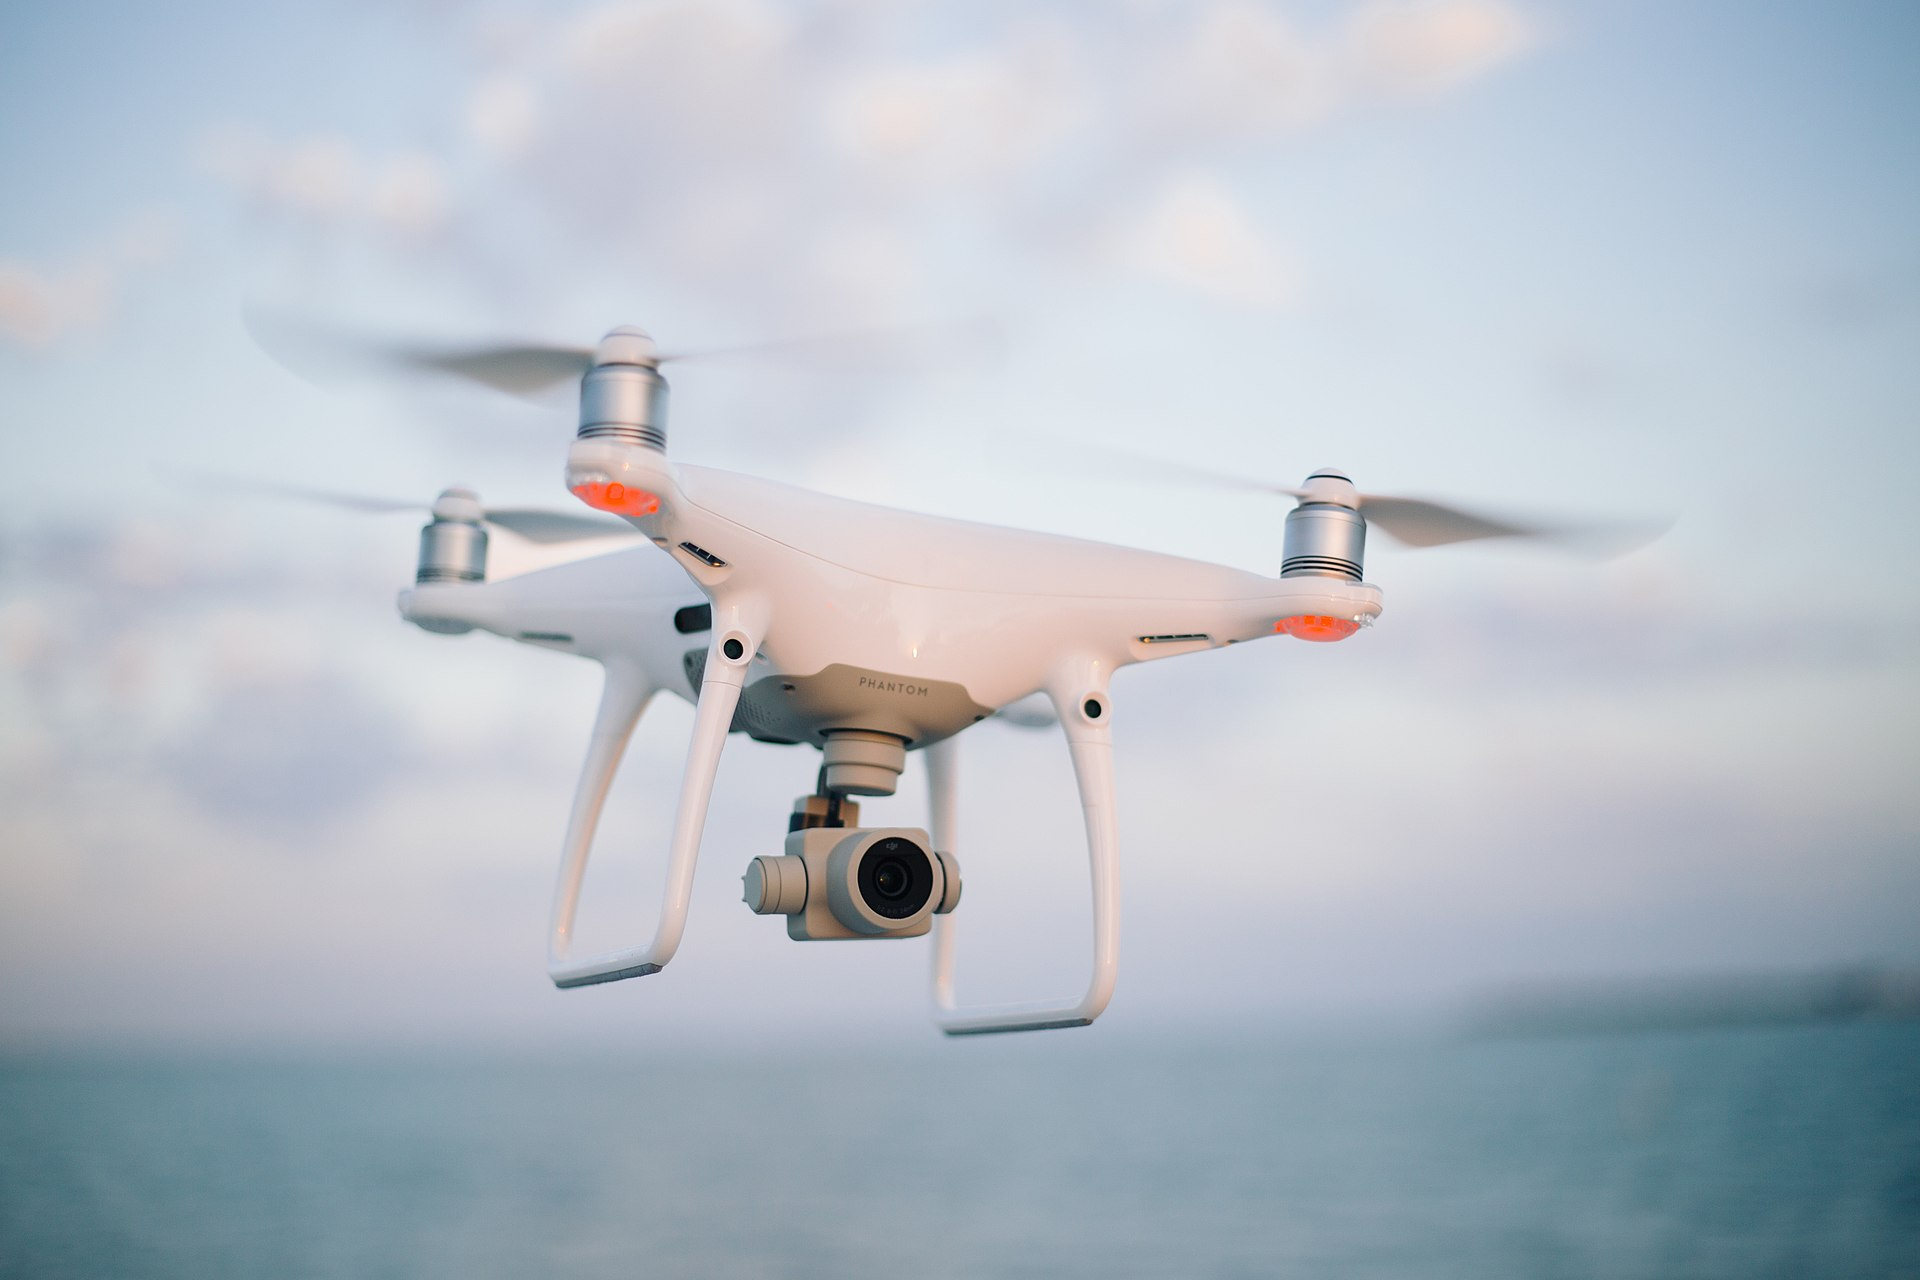
\includegraphics[width=\textwidth]{Images/Introduction/drone}
         \caption[Caption for LOF]{A DJI Phantom quadcopter (UAV)\protect\footnotemark}
         \label{fig:drone}
     \end{subfigure}
     \hfill
     \begin{subfigure}[b]{0.45\textwidth}
         \centering
         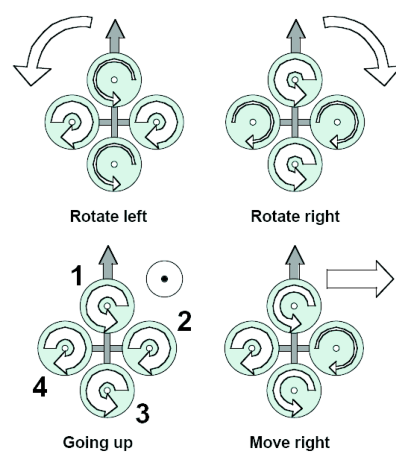
\includegraphics[width=0.6\textwidth]{Images/Introduction/propeller_direction.svg}
         \caption{Representation of the concept of a quadrotor. The width of the arrows is proportional to the angular speed of the propellers.\cite{Bouabdalla2007}}
         \label{fig:propeller_directions}
     \end{subfigure}
        \caption{A commercial quadrtotor platform with a representation of the quadrotor concept.}
        \label{fig:three graphs}
\end{figure}

\noindent The distinctive mechanical design of the quadrotor permits the actuation system to control all of the six degrees of freedom even though it is under-actuated. This is due to the fact that the rotational and translational dynamics are tightly coupled. Thus, all the translational and rotational motions can be carried off by properly controlling the magnitude and direction of the spinning speed of the rotors.   

\noindent \footnotetext[1]{\url{https://en.wikipedia.org/wiki/Quadcopter\#/media/File:Quadcopter_camera_drone_in_flight.jpg}, accessed on 01/08/2021.}


\pagebreak

Over the last few years, quadrotors have gained a large popularity in academia and in the industry. This is due to several reasons, such as: 

\begin{enumerate}

    \item Quadrotors are very simple to design and they can be easily assembled using relatively cheap components.  
    \item As quadrotors became more and more affordable and dependable, the number of real-world applications for quadrotors  has grown significantly. They are being used for aerial photography, agriculture, surveillance, inspection tasks, in addition to many other uses as well. 
    \item Quadrotors are quite agile and maneuverable during flight, especially when compared to other types of UAVs.
    
\end{enumerate}

However, one of the main challenges in the quadrotors community is the capability to design control and planning methods that will allow the quadrotors to carry out aggressive maneuvers.  The fast dynamics associated with typically small dimensions of such agile quadrotors, along with several aerodynamic effects that will become crucial during aggressive flight maneuvers, are just a few of the main problems that are faced during the system control design. Moreover, accurate tracking of the provided trajectory is a big issue in the case of aggressive maneuvers when the rotors are commanded high speeds and accelerations, which will cause rotors to become saturated and may also cause delays.


 \section*{Parallel manipulators}

A parallel manipulator is a mechanical system that consists of two connected platforms, the fixed platform and the moving platform. The latter is linked to the fixed platform thanks to at least two serial chains that are working in parallel. When compared to serial manipulators, parallel manipulators are more accurate and rigid. In addition, the ability to install the motors next to the fixed platform is a very important feature for them. Moreover, parallel manipulators can be used in a wide variety of applications that demand precision and high payload combined with high speed.\cite{Parallel_Manipulators}

\begin{figure}[h]
     \centering
     \begin{subfigure}[h]{0.45\textwidth}
         \centering
         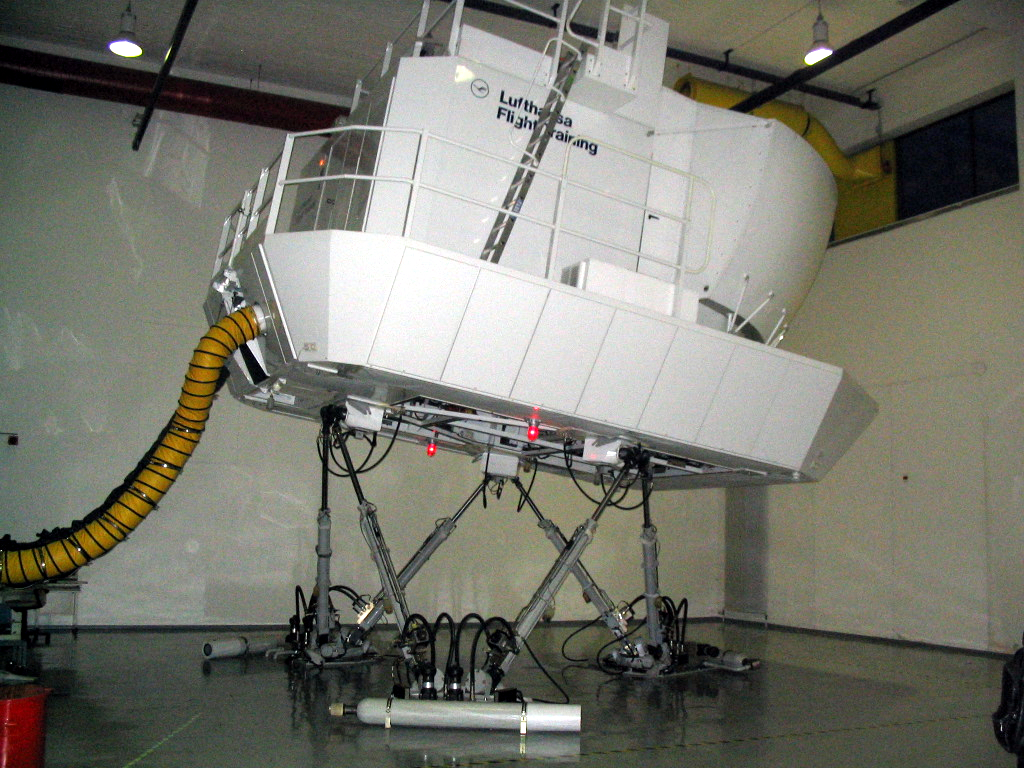
\includegraphics[width=0.7\textwidth]{Images/Introduction/GS}
    \caption[Caption for LOF]{Gough-Stewart used for a flight-simulator application.\protect\footnotemark}
         \label{GS}
     \end{subfigure}
     \hfill
     \begin{subfigure}[h]{0.45\textwidth}
         \centering
         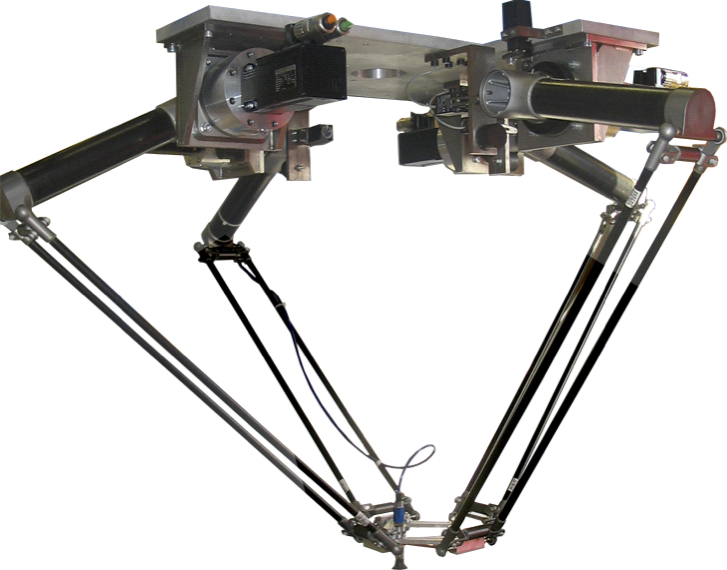
\includegraphics[width=0.7\textwidth]{Images/Introduction/PAR4}
         \caption[Caption for LOF]{The "PAR4" 4 degrees of freedom, high-speed, parallel robot prototype.\protect\footnotemark}
         \label{PAR4}
     \end{subfigure}
        \caption{Two examples of parallel robots.}
        \label{fig:three graphs}
\end{figure}




\footnotetext[1]{\url{https://en.wikipedia.org/wiki/Stewart_platform\#/media/File:Simulator-flight-compartment.jpeg}, accessed on 01/08/2021.}
\footnotetext[2]{\url{https://en.wikipedia.org/wiki/Parallel_manipulator\#/media/File:Prototype_robot_parall\%C3\%A8le_PAR4.jpg}, accessed on 01/08/2021.}


\pagebreak

However, parallel manipulators are subject to singularities which can lead to big problems in the robot workspace in case they were not handled correctly. Thus, the study of the singular configuartions of parallel manipulators is very important. Because, even just before reaching a singularity, the performance of the parallel manipulator will decrease dramatically. Moreover, the robot may loose the ability of moving in a certain direction, gain uncontrollable motions and the mechanism could even break. The main difference between serial and parallel manipulators is that singularity configurations may also appear inside the workspace of the robot (depending on the dimensions of the robot) and not just at the boundaries of the robot workspace, which can significantly decrease the area of the robot workspace.
As a result, many works have been developed by robotics researchers in order to allow parallel manipulators to safely cross these singularities by using trajectory planning and specific control methods.

\section*{The goal of this thesis}

This master thesis lies at the intersection of parallel robotics and aerial robotics. The two fields may seem very different from each other. However, quadrotors can be seen as a particular case of a parallel manipulator. 
In fact, a parallel manipulator is made up of a wrench system, applied by the robot limbs on the moving platform. And, this wrench system will define the motion of the moving platform. In the same manner, each propeller in a quadrotor can be considered as a limb of a parallel robot and the moving platform to be controlled can be considered as the body of the drone. 
Specifically, the goal of this master thesis is to study a distinct class of aggressive maneuvers for quadrotors, namely flip maneuvers. By doing flip maneuvers, full rotations around one or more axes of the body of the quadrotor can be done. In addition, the quadrotor should also be able to perform the flip maneuvers in constrained environments.

\begin{figure}[h]
     \centering
     \begin{subfigure}[h]{0.45\textwidth}
         \centering
         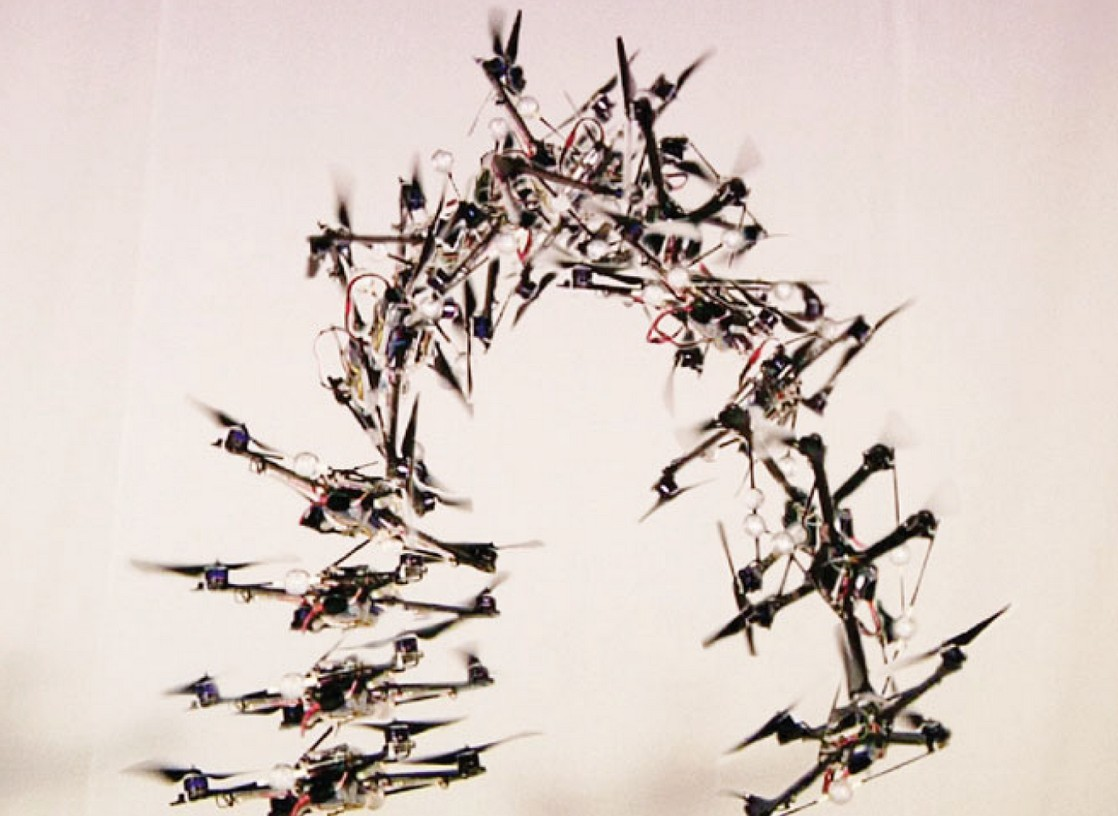
\includegraphics[width=0.9\textwidth]{Images/Introduction/flip}
    \caption{Quadrotor performing a triple flip.\cite{DAndrea2012}}
         \label{triple_flip}
     \end{subfigure}
     \hfill
     \begin{subfigure}[h]{0.45\textwidth}
         \centering
         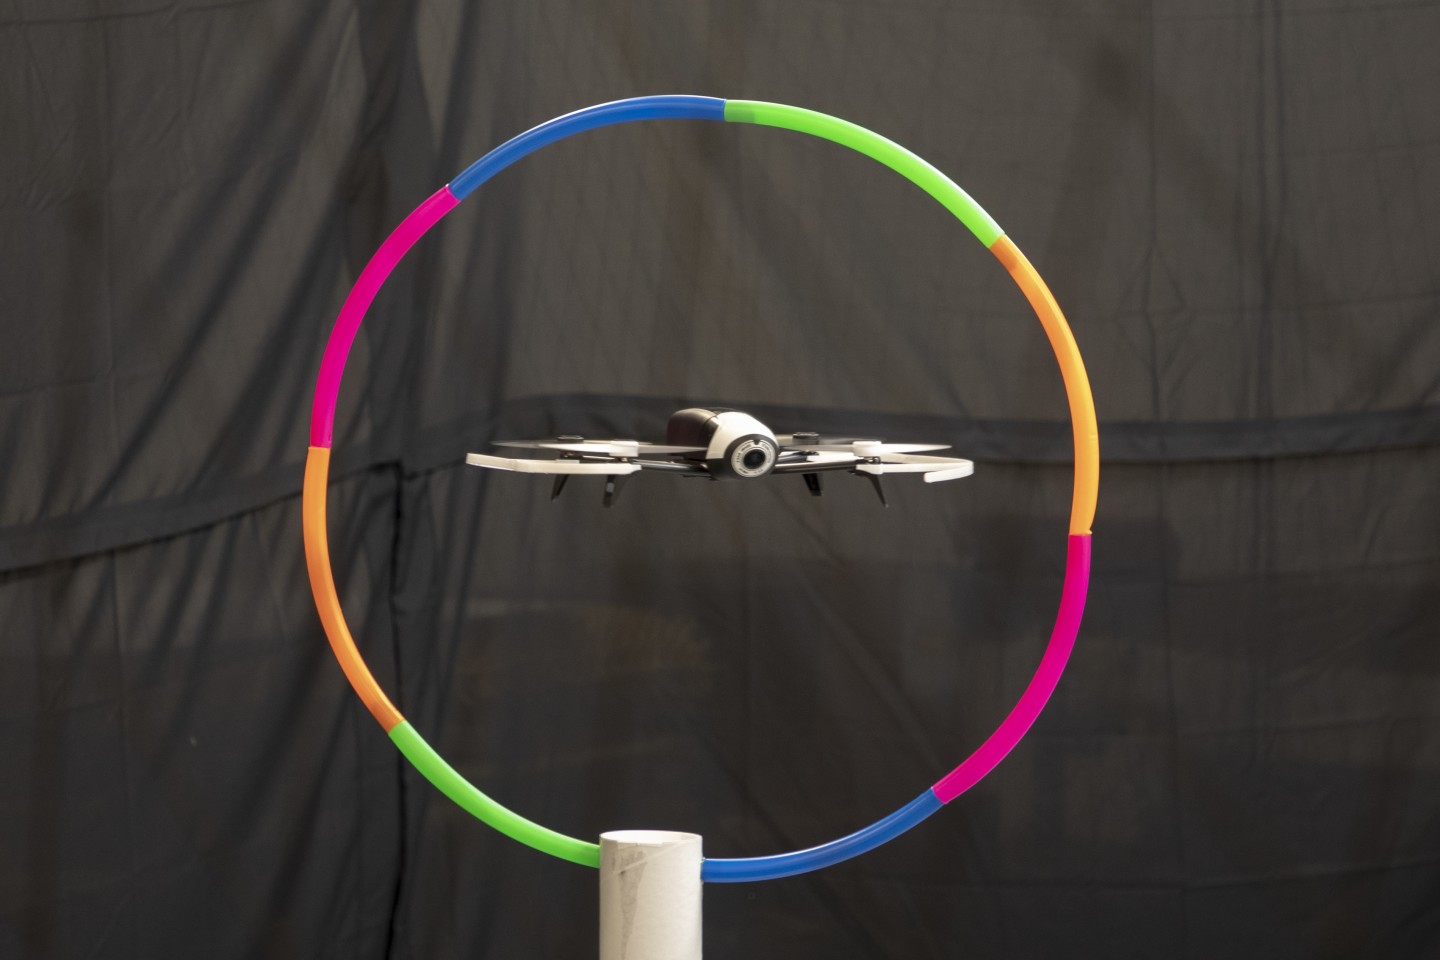
\includegraphics[width=\textwidth]{Images/Introduction/constrained_environment}
         \caption[Caption for LOF]{Quadrotor going though a loop.\protect\footnotemark[1]}
         \label{drone_hulahoop}
     \end{subfigure}
        \caption{Representation of the issues to be tackled in the master thesis.}
        \label{fig:three graphs}
\end{figure}

\footnotetext[1]{\url{https://newatlas.com/drones/muscle-signals-drone-control/\#gallery:2}, accessed on 01/08/2021.}

\pagebreak

\section*{Outline of the work}

The rest of the report is structured as follows:

\begin{comment}
\begin{itemize}
\setlength{\itemindent}{-.5in}
	\item [] \textbf{Chapter 1} is devoted to introduce the system modeling of quadrotors. Specifically, a simplified dynamic model of the quadrotor will be presented by using Euler-Lagrange formalism. Then, moving on from the simple dynamic model, a more detailed dynamic model will be presented by using the Newton-Euler formalism. Finally, the state-space model of the quadrotor will be derived.

	\item [] \textbf{Chapter 2} provides an overview of state of the art in quadrotor control in addition to introducing the different potential control methods that can be used during the master thesis in order to properly control the quadrotor. 

	\item [] \textbf{Chapter 3} provides detailed explanations of how multi-flip maneuvers can be handled. Then, the link between a quadrotor performing a flip and a parallel robot crossing a singularity will be explained. In the end, a literature review is provided in order to show how the problem is tackled by different researches.

	\item [] \textbf{Chapter 4} is devoted to trajectory optimization. By using trajectory optimization, it will be possible to create feasible trajectories for quadrotors to perform the aggressive maneuvers in constrained environments.
	
\end{itemize}
\end{comment}

\begin{itemize}
\setlength{\itemindent}{-.5in}
	\item [] \textbf{Chapter 1} provides an overview of the state of the art in the control of quadrotors and will later on focus on the main control method that will be used, namely Model Predictive Control (MPC). Moreover, a literature review of MPC applications on quadrotors will be presented. Furthermore, an overview on the software used to design a MPC controller will be presented. Finally, the state of the art in flipping maneuvers will be presented.
	
	 \item [] \textbf{Chapter 2} provides a detailed explanation of the quadrotor dynamics for the planar (2D) and 3D quadrotors. Morever, an Extended Kalman Filter (EKF) is then designed for the planar quadrotor case to be used in the presence of noisy measurements (states) and noisy control inputs. Finally, simulation results using MPC to reach a single waypoint and to follow circular trajectories with and without noise are presented.
	 
	 \item [] \textbf{Chapter 3} focuses on the trajectory generation of a flip trajectory where different optimization problems with different objective functions and initial conditions will be used in order to find the optimal flipping trajectory that satisfies the dynamic constraints of the quadrotor which will be used in the experimentation phase. Moreover, simulations with a MPC are then performed using the optimal flip trajectory.
	 
	 \item [] \textbf{Chapter 4} focuses on the simulations that were performed using ROS2 and Gazebo, in addition to the experimentation results.
\end{itemize}


\newpage
 
 \chapter{State of the art}
 
 In the following sections of this chapter, differential flatness,  the general control architecture of a quadrotor, different potential control approaches (linear and nonlinear), and the main control method that will be used to control a quadrotor, namely Model Predictive Control (MPC) will be explained. 
 \section{Differential Flatness}\label{Differential_flatness}  
 
 In the quadrotor community, a well-established finding is that the dynamic model of a quadrotor is differentially flat. Moreover, the control design problem in nonlinear systems will be considerably simplified. Precisely, a system with state $\textbf{\textsc{x}} \in \mathbb{R}^n$ and input $\textbf{\textsc{u}} \in \mathbb{R}^m$ is considered to be \textit{differentially flat} if there exists a set of \textit{flat outputs} $\textbf{\textsc{y}} \in \mathbb{R}^m$ which have the following form:
 
 \begin{equation}
 \textbf{\textsc{y}} = \textbf{\textsc{y}}(\textbf{\textsc{x}}, \textbf{\textsc{u}}, \dot{\textbf{\textsc{u}}},...,\textbf{\textsc{u}}^{(p)})
 \end{equation}

 With, 
 
 \begin{equation}
 	\begin{cases}
 		\textbf{\textsc{x}} = \textbf{\textsc{x}}(\textbf{\textsc{y}}, \dot{\textbf{\textsc{y}}},...,\textbf{\textsc{y}}^{(q)}) \\
 	\\
 		\textbf{\textsc{u}} = \textbf{\textsc{u}}(\textbf{\textsc{y}}, \dot{\textbf{\textsc{y}}},...,\textbf{\textsc{y}}^{(r)}) \\
 	\end{cases}
 \end{equation}

 As a result, the new set of variables is required to be a function of the state, the input and the derivatives of the input. Moreover, this set should also have the same dimensions as the control input. In this manner, it is possible to rewrite both the state and the input in function of the flat outputs and the derivatives of the flat outputs. This is a very useful property in underactuated systems where $m<n$, such as quadrotors, because, it will allow to generate trajectories in the lower dimensional space $m$, then this trajectory will be mapped into the full dimensional space $n$. An example of this is shown in figure \ref{fig:differential_flatness} below:
 
 \begin{figure}
 	\centering
 	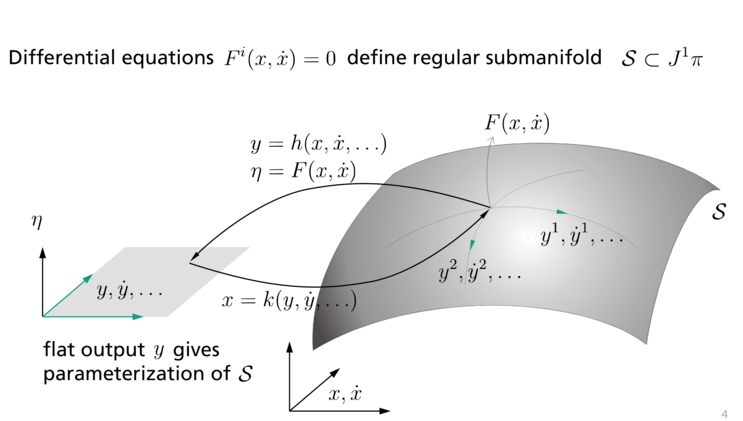
\includegraphics[width=0.7\textwidth]{Images/Control/differential_flatness.png}
 	\caption{Mapping between different dimensional spaces as a result of differential flatness. \cite{Fritzsche2019}}
 	\label{fig:differential_flatness}
 \end{figure}
 
 \newpage
 
 Another well known example of systems is a car, in which the underactuation is the result of the nonholonomic constraints that are imposed by the wheels. So, for a car, a generated trajectory for $(x,y)$ position of the rear-wheels is enough to specify all the viable trajectories of the system. Formal proofs that the quadrotor system is differentially flat can be found in \cite{Mellinger2011}, and \cite{Faessler2018} for the full model with first-order aerodynamics. The standard choice of flat outputs for the quadrotor is the coodinates of the center of mass and the yaw angle:

\begin{equation}\label{flat_outputs}
\textbf{\textsc{y}} = \begin{bmatrix}
x && y && z && \psi \\
\end{bmatrix}^{\intercal}
\end{equation}

Consequently, the problem of generating a feasible trajectory for a quadrotor then tracking it can be dimensionally decreased from a 6-dimensional space to a 4-dimensional space. By reason of the tight coupling between the rotational and translational dynamics, then defining a trajectory in function of the flat outputs $\textbf{\textsc{y}}$ is sufficient to properly define the full dynamics $\textbf{\textsc{x}}$.


\newpage

\section{General Control Architecture}
 Recently, many researchers have developed interest in the control of quadrotors. As a result, various control approaches have been proposed. The most known control architecture \cite{Faessler2018} consists of three nested control loops, as shown in figure \ref{fig:cascaded_pid_controller}, in order to generate the suitable motor commands to follow the desired signal. This controller is known as the cascaded controller. This strategy assumes that the attitude dynamics of a quadrotor are much faster than the translational dynamics. 
\begin{comment} 
Assuming that Euler angles are used to define the attitude and that a navigation module generates the desired trajectory $(\bm{r}_d(t),\psi_d(t))$ as shown in section \ref{Differential_flatness}, then:
 
\begin{itemize}
	\setlength{\itemindent}{-.5in}
	\item [] \textbf{Position controller} has the objective of driving the errors occurring on the translational dynamics to zero.
		And, the outputs of this outer loop are the thrust $f=u_1$, which is sent to the motor controller, and the desired attitude $(\theta_d(t),\phi_d(t))$, which corresponds to the reference signal of the attitude controller.
	\item [] \textbf{Attitude controller} has the goal of driving the errors occurring on the rotational dynamics to zero. This controller generates the inputs 
	$\bm{\tau}=\begin{bmatrix}
	u_2 && u_3 && u_4 \\
	\end{bmatrix}^{\intercal}
	$
	that are then sent to the motor controller.
	\item [] \textbf{Motor controller} This controller receives the control inputs 	$\bm{u}=\begin{bmatrix}
	f && \bm{\tau}
	\end{bmatrix}^{\intercal}
	$ and maps them into the desired spinning velocities $\Omega_i$ for each individual rotor. Moreover, low-level control laws are designed and realized in the firmware of the drone to make the convergence from the actual rotations to these desired values.
\end{itemize}
 

 
 \begin{figure}[h]
 \centering
 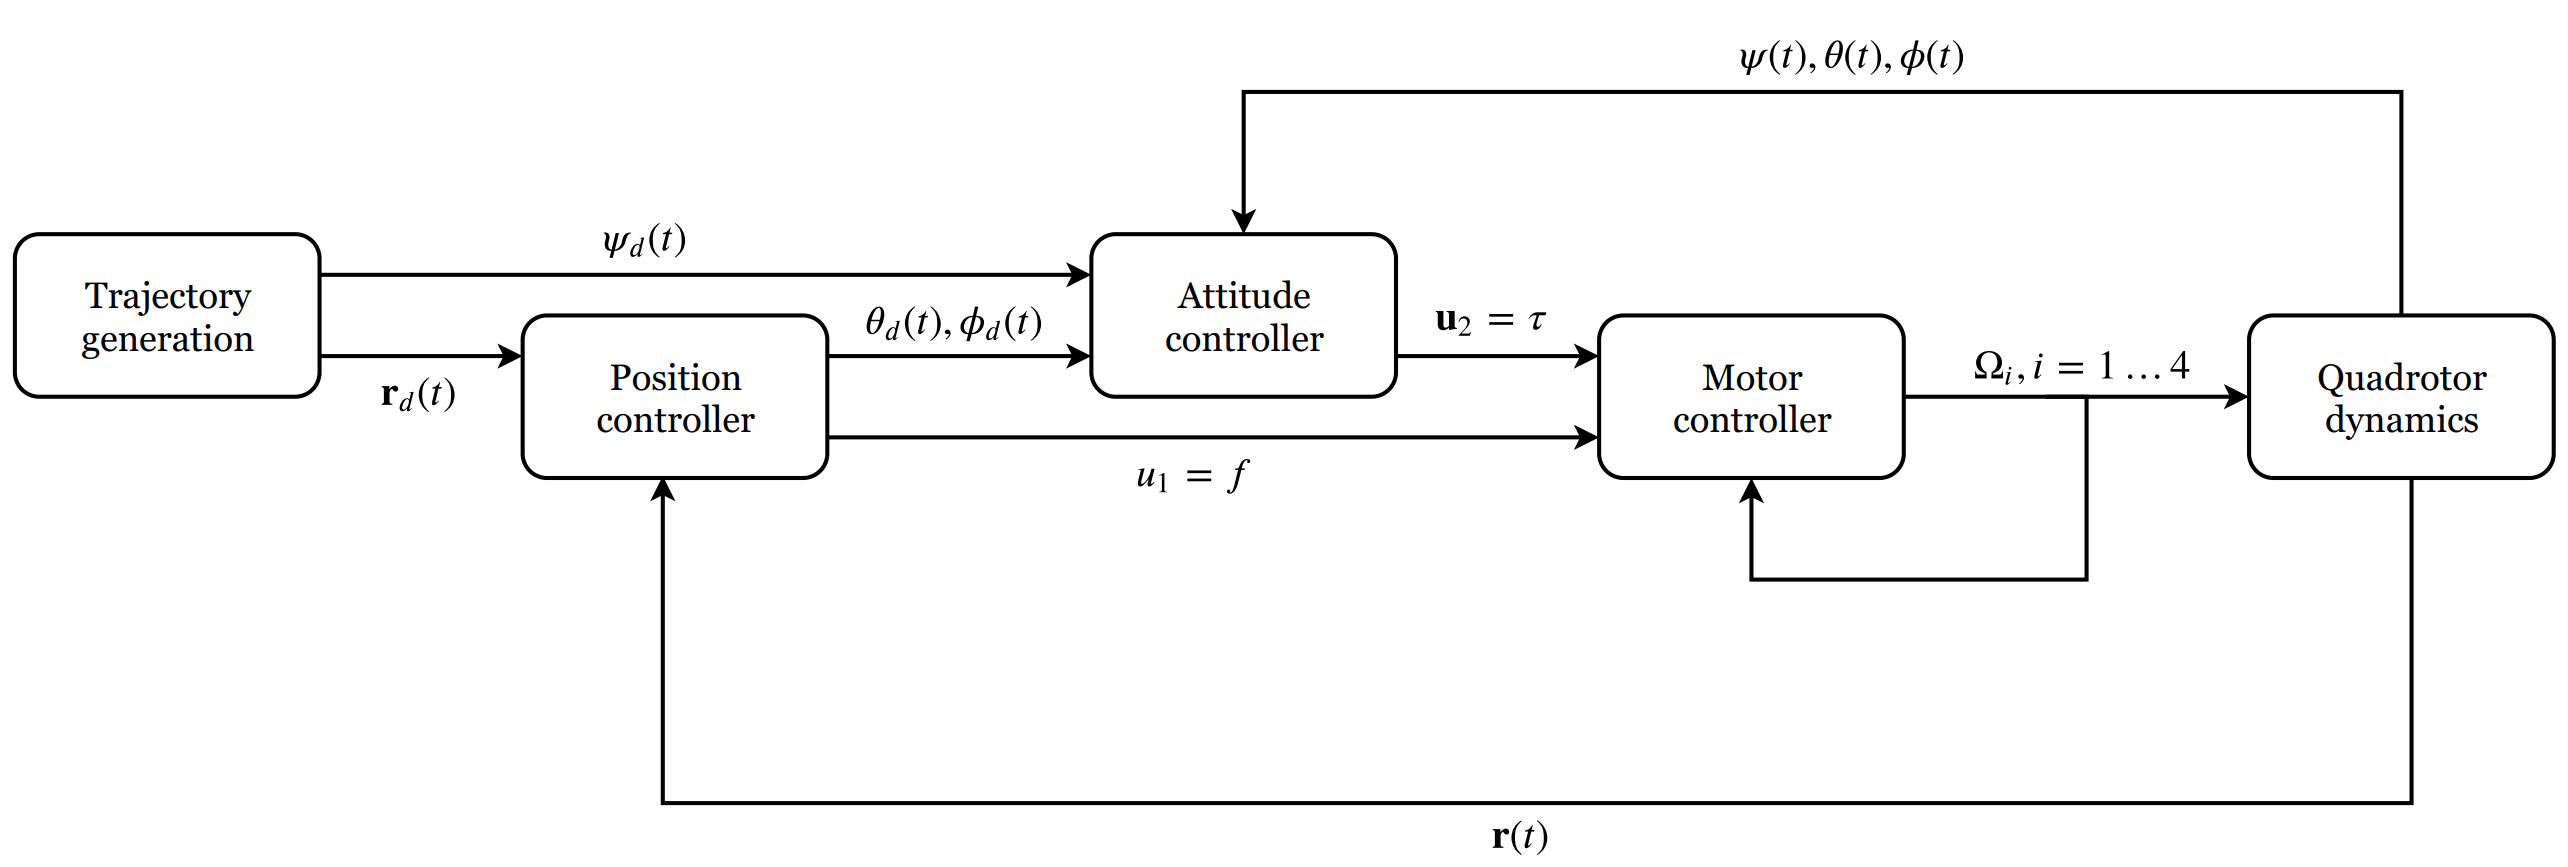
\includegraphics[width=0.8\textwidth]{Images/Control/General_control_architecture}
 \caption{Cascaded controller architecture.}
 \label{General_control_architecture}
 \end{figure}
 
There also exists different implementations of the cascaded controller that was shown in figure \ref{General_control_architecture}. An example of another architecture of a cascaded controller is shown below: 

\end{comment}



\begin{figure}[h]
	\centering
	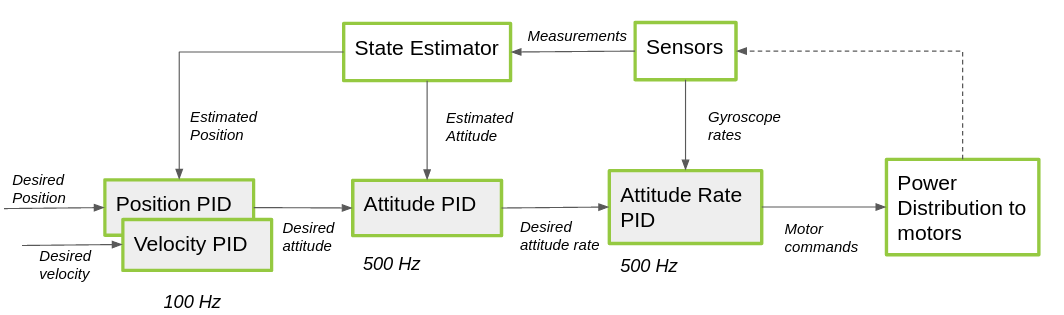
\includegraphics[width=\textwidth]{Images/Control/cascaded_pid_controller.png}
	\caption{Cascaded PID controller that is present on the crazyflie 2.1 quadrotor \cite{bitcraze}.}
	\label{fig:cascaded_pid_controller}
\end{figure}

In this case, the position and velocity controller, attitude controller and attitude rate controller are all PID controllers. And, it is evident that the attitude dynamics (who's attitude and attitude rate controllers operate at a frequency of 500Hz) are considered to be much faster than the translational dynamics (who's position and velocity controllers operate at a frequency of 100Hz). Moreover, 

\begin{itemize}
	\setlength{\itemindent}{-.5in}
	\item [] \textbf{Attitude Rate PID controller} directly controls the attitude rate. It receives the gyroscope rates after they have been filtered and uses the error between the desired attitude rate and current attitude rate, and outputs the motor commands which are then directly sent to the power distribution.
	
	\item [] \textbf{Attitude PID controller} directly controls the attitude of the drone. It takes the estimated attitude from the state estimator and uses the error between the desired attitude and the current attitude to output the desired attitude rate.
	
	\item [] \textbf{Position and Velocity PID controller} is the most outerloop of the cascaded PID controller. It receives the position or the velocity input from the high level commander which are then handled to output the desired attitude.
	 
\end{itemize}

 \newpage 
\section{General Control Approaches}\label{control_approaches_for_multi_flip_maneuvers}

\subsection{Method of Linearization}

By using extreme assumptions, it is feasible to apply linear control techniques in order to control a quadrotor (\cite{Sabatino2015}, \cite{BouabdallahNothSiegwart2018}). Particularly, this can be made by doing a linearization of the full dynamic model around an equilibrium point $\overline{\textbf{\textsc{x}}}$ and by using the assumption that the vehicle is only capable of oscillating lightly around the hover point.
It is very easy to observe that a feasible equilibrium is provided by a configuration where the center of mass is at a random position $\overline{\textbf{\textsc{r}}}$ and all the other elements of the state are set to zero. So, the nominal input $ \textbf{\textsc{u}} = \overline{\textbf{\textsc{u}}}$ to sustain such equilibrium can be assessed as the thrust that is required to compensate the gravity force:

\begin{equation}
\overline{\textbf{\textsc{u}}} = \begin{bmatrix}
f \\ 
\bm{\tau}\\
\end{bmatrix}=
\begin{bmatrix}
mg \\
\bm{0_{3 \times 1}} \\
\end{bmatrix}
\end{equation}

At this stage, the complete non-linear dynamics that have the form :

\begin{equation}
\dot{\textbf{\textsc{x}}}=\overline{\textbf{\textsc{f}}}(\overline{\textbf{\textsc{x}}},\overline{\textbf{\textsc{u}}})
\end{equation}

can now be linearized around the hover point $(\overline{\textbf{\textsc{x}}},\overline{\textbf{\textsc{u}}})$ as shown below.

\begin{equation}
\dot{\textbf{\textsc{x}}} = \begin{bmatrix}
\frac{\partial \textbf{\textsc{f}}(\textbf{\textsc{x}},\textbf{\textsc{u}})}{\partial \textbf{\textsc{x}}}
\end{bmatrix}_{(\bar{\textbf{\textsc{x}}},\bar{\textbf{\textsc{u}}})} \textbf{\textsc{x}}+ 
\begin{bmatrix}
\frac{\partial \textbf{\textsc{f}}(\textbf{\textsc{x}},\textbf{\textsc{u}})}{\partial \textbf{\textsc{x}}}
\end{bmatrix}_{(\bar{\textbf{\textsc{x}}},\bar{\textbf{\textsc{u}}})} \textbf{\textsc{u}} = \textbf{\textsc{A}}\textbf{\textsc{x}} + \textbf{\textsc{B}} \textbf{\textsc{u}}
\end{equation}

It can be demonstrated that both matrices $\textbf{\textsc{A}}$ and $\textbf{\textsc{B}}$ can be used to determine a linear system that is both controllable and observable \cite{Sabatino2015}. Thus, any control technique that is linear can now be used on the quadrotor in order to keep it around a desired equilibrium point, such as optimal LQR/LQG \cite{Cowling2007,Minh2010} control or simple PD or PID controller \cite{Han2012,Altug2007}.


 \subsection{Nonlinear Control Methods}
 

In order to perform more complex tasks and follow aggressive trajectories, nonlinear control methods are required.
A comprehensive literature review on this topic is beyond the scope of this work and several works can be found, such as \cite{Zulu2016}, which provides a general overview on nonlinear control of quadrotors. However,
some nonlinear control methods deserve to be mentioned due to their extensive use and applications:

\begin{itemize}
\setlength{\itemindent}{-.5in}

	\item [] \textbf{Sliding Mode control} It is a control technique that is nonlinear presenting exceptional attributes of robustness,accuracy, easy tuning and execution. The aim of SMC systems is to drive the system states to a specific surface in the state space, called  \textit{"sliding surface"}. Upon reaching the sliding surface, sliding mode control allows the states to remain on the close neighborhood of the sliding surface. Therefore, the sliding mode control consists of a controller design with two parts. The first part contains the design of a sliding surface in order for the sliding motion to fulfill design requirements. The second deals with selecting a control law that makes the switching surface interesting with respect to the system state \cite{Utkin1997}.
There exist two main benefits of sliding mode control. Firstly, the behavior of the dynamics of the system can be changed according to a specific selection of the sliding function. Secondly, the response of the closed loop system becomes completely insensitive to some special uncertainties. This principle goes beyond bounded model parameter uncertainties, interference and non-linearity. In a practical sense, SMC allows the control of nonlinear processes that are affected by external noise and heavy model uncertainties.
The most important principles of SMC are shown in the following significant references \cite{Utkin1997,DeCarlo1998,Hung1993}. Researchers have also studied the problems appearing in the practical execution of this class of techniques. \cite{Young1999}
Interested readers can refer to the book \cite{Bartolini2008} which presents a very modern overview of the most promising current line of theoretical and practical research in the domain.

	\item [] \textbf{Backstepping control} The main idea is to divide the system into successive subsystems and to apply a recursive algorithm which will stabilize each subsystem after the other \cite{Madani2006}. However, this method is not robust, but it is computationally fast. In order to handle disturbances, Fang et al. \cite{Gao2011} implemented an integral backstepping control law, in which the integral term was shown to reduce steady state errors and the response time of the system greatly. 

	\item [] \textbf{Adaptive control} This method is required when the parameters that are characterizing the system contain errors or are unknown. This type of control algorithms contains a parameter adaptation law, which is enclosed in the control to track the desired trajectory of the system, even if the model of the system is not completely known.
For instance, Diao et al. \cite{Diao2011} obtained good performance even though the inertial parameters of the quadrotor and the aerodynamic coefficients were not perfectly known. This method is convenient in some cases, such as the existence of unpredictable wind \cite{Antonelli2013} or pick-and-place applications with small loads. 
	 
 \end{itemize}
 

In the next section, the main control method that will be used in the master thesis will be explained.

\newpage

\section{Model Predictive Control}

\subsection{General Idea}\label{MPC_General_Idea}
 
 There exist "open-loop" methods \cite{Kirillova2000} in which the control input sequence $\textbf{\textsc{u}}(t)$ is designed using a model of the system and a set of constraints. However, the problem with this approach is that modeling errors and noise are not taken into consideration. So, these inputs will not necessarily generate the desired response from the system. Because of that, a \textit{"closed-loop"} strategy is required in order to cancel out these errors. So, an approach that can be used is called \textit{"Model Predictive Control"} (MPC). This method is also known as \textit{"receding horizon control"} \cite{How2008} because the \textit{"prediction horizon"} (which is a finite horizon) translates forward by one time step after the current optimization problem is solved . In short, MPC is a \textit{feedback control} algorithm which uses a model of the system to predict the future outputs of the system and it solves an optimization problem on-line in order to select an optimal control.
 
 \paragraph{Basic strategy}

The basic strategy of MPC is the following:


\begin{itemize}
	\item At time step $k$, the system model and an optimizer will be used in order to design a sequence of control inputs
	
	$$ \textbf{\textsc{u}}(k|k), \textbf{\textsc{u}}(k+1|k), \textbf{\textsc{u}}(k+2|k), \textbf{\textsc{u}}(k+3|k),...,\textbf{\textsc{u}}(k+N|k) $$
	
	starting from the current state $\textbf{\textsc{x}}(k)$ over a prediction horizon $N$.
	\item Only the first step of the sequence of control inputs will be applied on the system.
	\item The processes above are then iterated for time $(k+1)$ at state $\textbf{\textsc{x}}(k+1)$. 
\end{itemize}
 
 
 \begin{figure}[h]
 \centering
 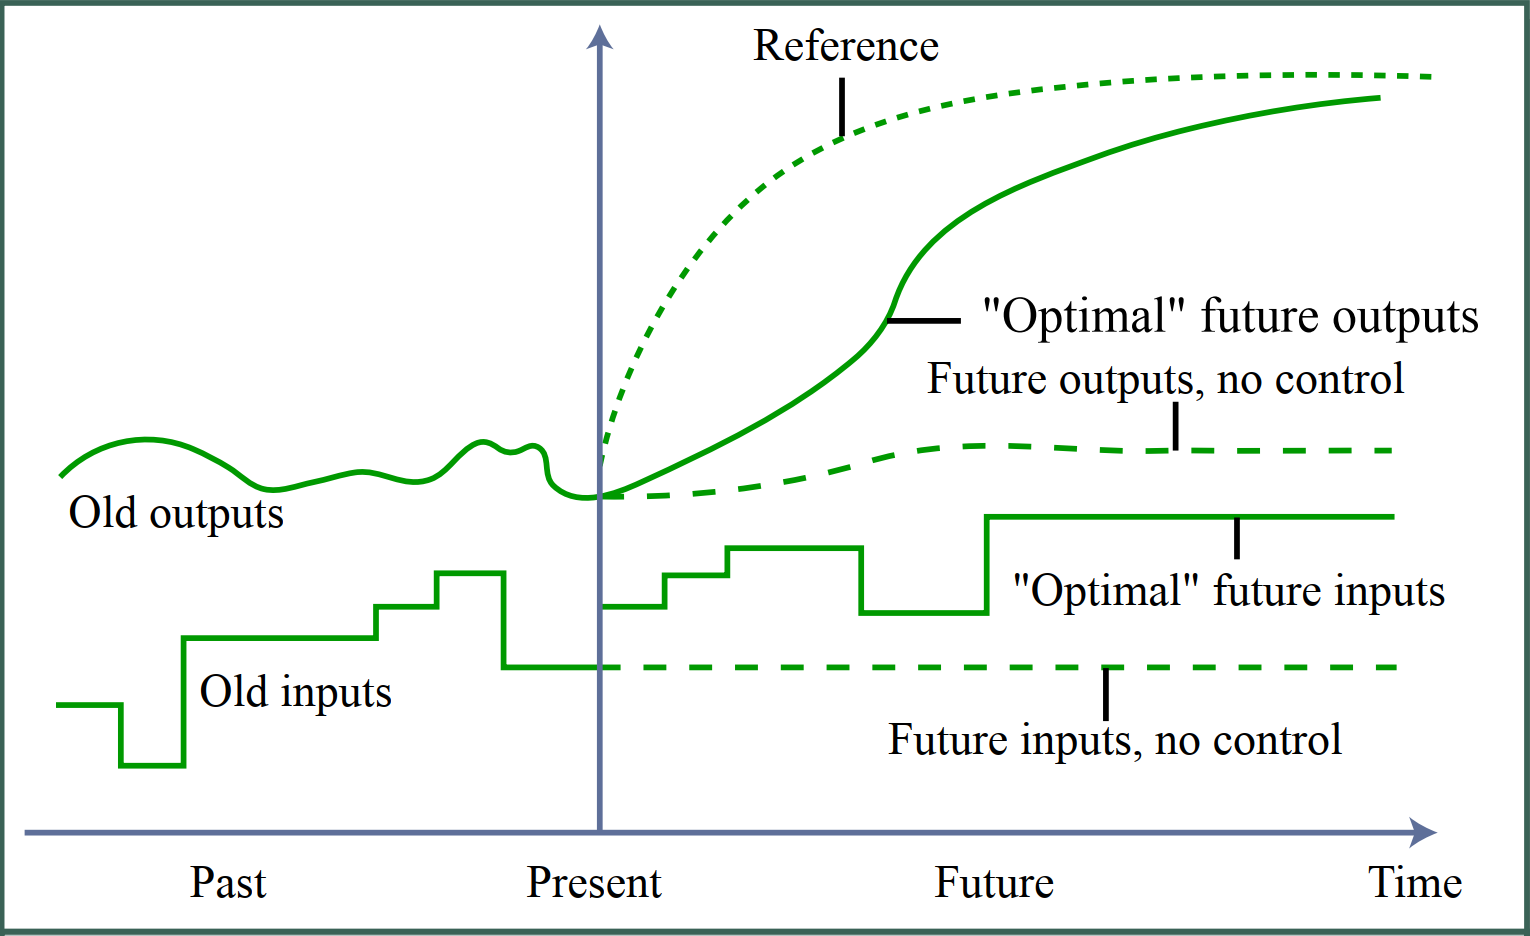
\includegraphics[width=0.6\textwidth]{Images/Control/MPC_general_idea.png}
 \caption{Basic idea of MPC \cite{How2008}.}
 \label{MPC_basic_idea}
\end{figure}  
 
\noindent It should be noted that the control algorithm of MPC is based on numerically solving an optimization problem at each time step. And, it is a constrained optimization in general.
 
 \paragraph{Advantages and drawbacks of MPC} There are several advantages when using MPC: 
 
 \begin{itemize}
 	\item MPC is able to control multi-input multi-output (MIMO) systems which might have interactions between their inputs and outputs.
 	\item MPC explicitly accounts for the constraints that are imposed on the system. So, it does not just design a controller to keep the system away from the constraints.
 	\item MPC can easily handle nonlinear dynamics and time-varying plant dynamics, because the controller is explicitly a function of the model of the system which can be modified in real-time.
 \end{itemize}

\noindent The main drawback of MPC is that it usually requires a powerful and fast processor with a large memory in order to properly solve the problem at hand. This is because MPC solves an optimization problem at each time step.
 
\noindent There have been many commercial applications of MPC starting from the early 1970s in the process industry. The table \ref{table_MPC} below shows the different companies that have used MPC in different industries in 2014.
 

\begin{table}[h]
\setlength{\tabcolsep}{15pt} % Default value: 6pt
\renewcommand{\arraystretch}{1} % Default value: 1
 \caption{The number of MPC applications in different industries in 2014 \cite{Kozak2014}.}
 \label{table_MPC}
\begin{tabular}{l c c c c c r}
Application & Aspen & Honeywell & Adersa & CCI & Pavilion & Total \\
\hline
Refining & 950 & 300 & 290 & - & 15 & 1555 \\
Chemicals & 437 & 55 & 12 & 21 & 25 & 550 \\
Food & - & - & 48 & - & 14 & 62 \\
Pulp paper & 21 & 39 & - & - & 3 & 63 \\
Gas and air & 11 & 13 & - & 24 & - & 48 \\
Polymer & 5 & - & - & - & 22 & 27 \\
Utilities & 7 & 9 & - & 6 & - & 22 \\
Other & 39 & - & 51 & 6 & - & 96 \\
\hline 
\hline
Total & 1470 & 416 & 401 & 57 & 79 & 2423 \\
\end{tabular}
\end{table}

\noindent However, as computational power has increased throughout the years thanks to the advancement of technology, there has been a renewed curiosity in applying this control approach to systems with fast dynamics for which the computational complexity is significantly larger when compared to the industrial applications for which computational complexity was not a concern (since MPC was applied on systems with slow dynamics in that case).
 
\subsection{Design Parameters}\label{design_parameters}
The different parameters that can be tuned in a MPC controller (\cite{MathWorks2018, MathWorks2018b, MathWorks2018c}) are the following:

\begin{itemize}
	\item The sample time $T_s$.
	\item The prediction horizon $N$.
	\item The control horizon $m$.
	\item The constraints.
	\item The weights.
\end{itemize}

\noindent Choosing the proper values for the parameters stated above is very important since they affect the performance of the controller and the computational complexity of the MPC algorithm.

\paragraph{Sample Time $T_s$} 

The sample time determines the rate at which the controller executes the control algorithm. \begin{itemize}
	\item If $T_s$ is too large, then when disturbances occur, the controller will be unable to react to the disturbances quickly enough.
	\item If $T_s$ is too small, the controller will have much faster reaction times to disturbances and set-point changes. However, this comes at the cost of an excessive computational load.
\end{itemize}

\noindent In order to find reasonable balance between controller performance and computational effort, the general recommendation is to have between 10\% and 25\% of the minimum desired closed-loop response time .

\paragraph{Prediction horizon $N$} 

The prediction horizon $N$ (sometimes referred to with the variable $p$, however, $N$ will be used instead for the remaining of this report) is the number of predicted future time steps of the system. It shows how far the controller predicts into the future. Thus, a prediction horizon must be chosen in such a way that it covers the significant dynamics of the system. However, it should be noted that a large prediction horizon should not be selected, since unexpected phenomenons could occur that may affect the dynamics of the system, which will cause a waste of computational power. The general recommendation is to increase $N$ until additional increases will have little impact on the performance. The maximum $N$ is the number of control intervals needed for the open-loop step response of the system to become infinite. However, having $N>50$ is hardly ever required unless $T_s$ is very small.

\paragraph{Control horizon m}

The control horizon is the set of future actions which will lead to the predicted plant output. It represents the number of control moves until time step $m$. After the first $m$ steps, the remaining inputs will remain constant as shown in figure \ref{MPC_basic_idea} for the \textit{"Optimal"} future inputs. Moreover, each control input element in the control horizon is a free variable that will be computed by the optimizer. Thus, the smaller the control horizon, the fewer the computations. However, setting $m=1$ may not give the best possible output for the system. And, similarly to the prediction horizon, if the control horizon is increased, this will lead to better predictions at the cost of increasing the computational complexity. Moreover, the general recommendation for the control horizon is to keep it much smaller than the prediction horizon, because:

\begin{itemize}
	\item A smaller control horizon $m$ will lead to less variables to optimize in the QP that will be solved at each control input interval. This will encourage quicker computation times.
	\item If delays are considered, then having $m<N$ is mandatory. Otherwise, some control input elements within the control horizon  may not have any effect on the plant outputs before the prediction horizon ends, which will lead to a QP Hessian matrix which is singular. 
	\item Having a small value for $m$ encourages having an internally stable controller. However, this is not guaranteed.
\end{itemize}

\paragraph{Constraints} A model predictive controller can integrate constraints on the inputs, the rate of change of the inputs and the outputs. In addition, the constraints can be \textit{"soft"} constraints or \textit{"hard"} constraints. \textit{"Soft"} constraints represent constraints that are allowed to be violated if the MPC deems it to be necessary in order to find a solution for the control problem at hand.
In addition, it should be noted that \textit{hard} constraints are a set of constraints that cannot be violated by the MPC. However, applying hard constraints on both the inputs and outputs at the same time may cause conflicts to occur between the constraints, which may lead to an unfeasible solution. Moreover, the general recommendation is to use soft constraints on the outputs and to avoid having hard constraints on both the inputs together with the rate of change of the inputs.

\paragraph{Weights} Model Predictive Control could have many goals. A possible goal could be to have the outputs converge to their set-points as fast as possible. Another goal could be to have smooth control inputs in order to avoid aggressive control maneuvers. So, in order to achieve a balanced performance between these two competing goals, the input rates and the outputs can be weighted relatively to each other. It is also possible to adjust relative weights within the input rates and the outputs.

\subsection{Basic formulation of a MPC problem} 

For a given set of plant dynamics which is first assumed to be linear:

\begin{equation}
\begin{cases}
\textbf{\textsc{x}}(k+1) = A\textbf{\textsc{x}}(k) + B \textbf{\textsc{u}}(k) \\
\textbf{\textsc{z}}(k) = C \textbf{\textsc{x}}(k)\\
\end{cases}
\end{equation}

\noindent and a cost function as follows: 

\begin{equation}
J = \sum_{j=0}^{N} \{ \|\textbf{\textsc{z}}(k+j|k)\|_{R_{zz}} + \|\textbf{\textsc{u}}(k+j|k)\|_{R_{uu}} \} + F \textbf{\textsc{x}}(k+N|k))
\end{equation}

 
\noindent With: 
 
 \begin{itemize}
 	\item $\|\textbf{\textsc{z}}(k+j|k)\|_{R_{zz}}$ is the weighted $L^2$-norm of the state, so it is expressed as follows:

 \begin{equation*}
 \|\textbf{\textsc{z}}(k+j|k)\|_{R_{zz}} = \textbf{\textsc{z}}(k+j|k)^{\intercal}R_{zz}\textbf{\textsc{z}}(k+j|k)
\end{equation*}   	
 	
	\item  	$\|\textbf{\textsc{u}}(k+j|k)\|_{R_{uu}}$ is the weighted $L^2$-norm of the control input sequence, so it is expressed as follows:
	
\begin{equation*}
 \|\textbf{\textsc{z}}(k+j|k)\|_{R_{zz}} = \textbf{\textsc{z}}(k+j|k)^{\intercal}R_{zz}\textbf{\textsc{z}}(k+j|k)
\end{equation*}  

	\item $F \textbf{\textsc{x}}(k+N|k))$ is a terminal cost function which can also have weights if required.
 	
\end{itemize}  
 
It should be noted that if  $N \rightarrow \infty$, and there are no additional constraints on  $\textbf{\textsc{z}}$ and/or $\textbf{\textsc{u}}$, then the problem falls back to the discrete LQR problem \cite{Kostova2013}. Moreover, when limits are added on 
  $\textbf{\textsc{x}}$ and/or $\textbf{\textsc{u}}$, then the general solution cannot be found anymore in analytical form, and it has to be solved numerically.

Furthermore, solving for a very long sequence of control inputs is irrelevant if the model used for the computations is expected to be erroneous or there are disturbances applied on the system, since only the first element of the optimized control sequence will be implemented. This is why MPC is generally designed by using a relatively small $N$.
  
  \paragraph{Typical problem statement}
  
  For a finite $N$ and with $F=0$ the problem can be expressed as follows: 
  
\begin{mini}|s|
{u}{ J = \sum_{j=0}^{N}{  \{ \|\textbf{\textsc{z}}(k+j|k)\|_{R_{zz}} + \|\textbf{\textsc{u}}(k+j|k)\|_{R_{uu}} \} }}
{}{}
\addConstraint{ \textbf{\textsc{x}}(k+j+1|k) = A\textbf{\textsc{x}}(k+j|k) + B \textbf{\textsc{u}}(k+j|k) }
\addConstraint{ \textbf{\textsc{x}}(k|k) \equiv \textbf{\textsc{x}}(k) }
\addConstraint{\textbf{\textsc{z}}(k) = C \textbf{\textsc{x}}(k+j|k)}
\addConstraint{|\textbf{\textsc{u}}(k+j|k)| \leq u_{max}}
{}
\label{optim_problem}
\end{mini}


\subsection{Different MPC Methods}\label{different_mpc_methods}
The MPC methods that are mainly used are the following:

\begin{itemize}
	\item Linear time-invariant MPC.
	\item Adaptive MPC.
	\item Gain-Scheduled MPC.
	\item Non-linear MPC.
\end{itemize} 

\noindent The method to be used is chosen based on the complexity of the system at hand and on the required goals to be reached. 

\paragraph{In case of linear systems} The method to be used is called linear time-invariant MPC. The constraints must be linear and the cost function must be quadratic. These characteristics will result in a convex optimization problem \cite{ZEMAN2003325} which has a global optimum. An example of a convex function is shown in figure \ref{convex_function} below.

\begin{figure}[h]
\centering
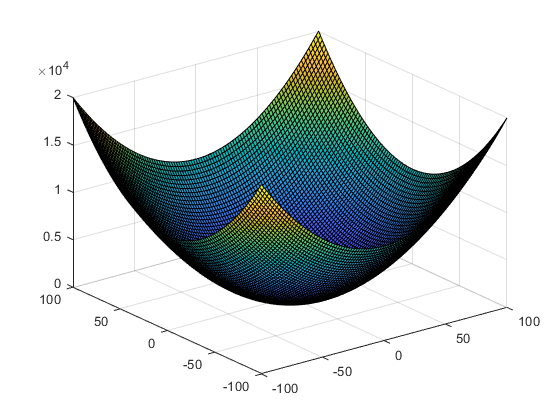
\includegraphics[width=0.6\textwidth]{Images/Control/MPC_Convex_Equation}
\caption{Representation of a convex function.}
\label{convex_function}
\end{figure}

\paragraph{In case of a nonlinear systems} If the system is linearizable, then both Adaptive MPC and Gain-Scheduled MPC can be used in this case. But the constraints are still linear and the cost function is still quadratic. In this case, the nonlinear function can be linearized around an operating point, which will result in a linear function that approximates the nonlinear system well near the operating point. However, it should be noted that the linear function will not work well outside the operating region. This is why it is interesting to find multiple linearized models, with each model representing the nonlinear function well around it's operating point.



\begin{figure}[h]
\centering
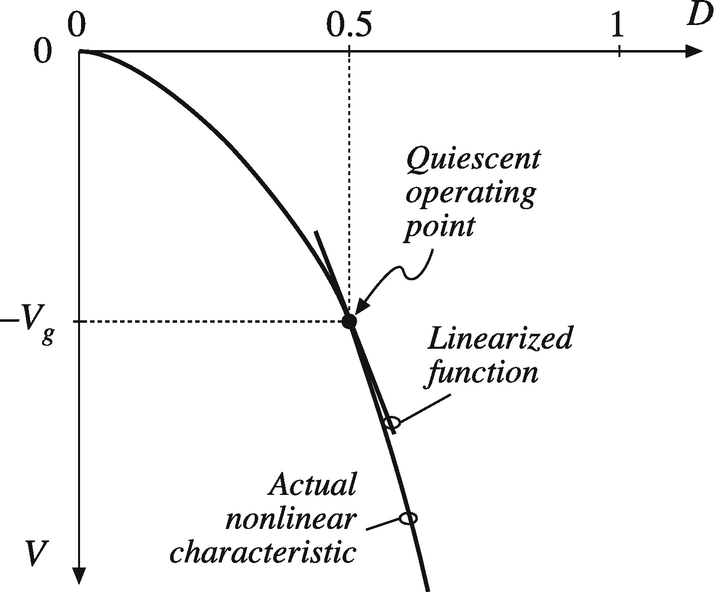
\includegraphics[width=0.45\textwidth]{Images/Control/linearization}
\caption{Example of the linearization of a nonlinear function around an operating point \cite{Erickson2020}.}
\label{nonlinear_function_linearization}
\label{non_convex_function}
\end{figure}



\paragraph{Adaptive MPC} In this case, a linear model is computed on-line as the operating conditions change. And, the internal plant model used by the MPC is updated with the corresponding linear model at each time step. Moreover, it should be noted that the optimization problem remains the same across different operating points. In other words, the number of elements in the state and the constraints remain the same across different operating conditions \cite{Bujarbaruah2018}.

\paragraph{Gain-Scheduled MPC} In this case, linearization of the nonlinear model is done offline at the operating points of interest. Then, a linear MPC controller is designed for each operating point. However, it should be noted that unlike Adaptive MPC, each controller is now independent from the other. In other words, the number of elements in the state and the constraints are different across different operating conditions.
It should also be noted that for this method, an algorithm must be designed to switch between the predefined MPC controllers for different operating conditions. Moreover, Gain-Scheduled MPC also uses more memory than Adaptive MPC \cite{7347864}.

\paragraph{Nonlinear MPC} If the system is nonlinear and cannot be linearized, and both the constraints and the cost function are also nonlinear, then nonlinear MPC can be used in that case. It is the most powerful method of all the different methods mentioned earlier, since it uses the most accurate representation of the plant. Thus, predictions are more accurate. However, nonlinear MPC is the most difficult method to solve in real-time. Because, in that case the problem becomes a non-convex optimization problem. Thus, the cost function may have many local minima, and finding the global minimum may be hard in that case. An example of a non-convex function is shown in figure \ref{nonconvex_function} below.


\begin{figure}[h]
\centering
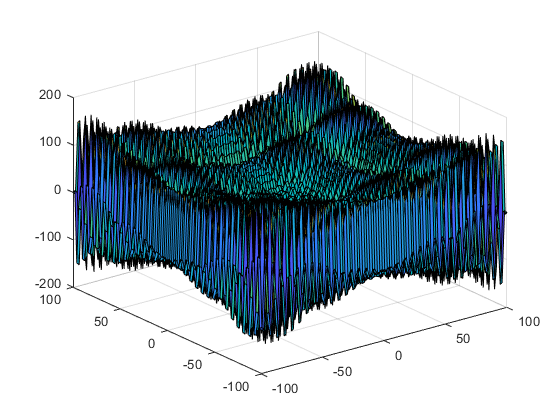
\includegraphics[width=0.6\textwidth]{Images/Control/MPC_Nonconvex_Equation_b}
\caption{Representation of a non-convex function.}
\label{nonconvex_function}
\end{figure}

\subsubsection{Strategies to Improve Computational Time}

As demonstrated in (\ref{MPC_problem}), an MPC problem is formulated as a QP problem that tries to minimize a quadratic cost function in general. Moreover, MPC computations become more complex as the number of state elements, the number of constraints and the MPC parameters increase. Moreover, as stated in section \ref{MPC_General_Idea}, if the MPC controller is running on applications with slow dynamics, then computational complexity is not a concern. However, if MPC is running on applications with fast dynamics, then the computational complexity becomes crucial. In addition, it is important to note that the matrices that are stored in the processor of the system for MPC computations grows with the increasing number of optimization variables. Thus, this could cause a memory problem. So, to reduce the complexity and computational time of MPC, the following methods can be used:

\paragraph{Order reduction techniques} They are used to discard states that do not contribute to the dynamics of the system \cite{4421358}. And, using order reduction techniques will also reduce the memory usage of the controller.

\begin{comment}
\paragraph{For applications with small $T_s$} In these cases, the performance of the MPC controller can be increased by \cite{bequette2003process}:
\begin{itemize}
	\item Shortening the prediction horizon.
	\item Shortening the control horizon.
	\item Reducing the number of constraints.
	\item Having lower precision operations and data representation.
\end{itemize} 
It should be noted that for applications with even smaller sample times, \textit{Explicit} MPC can be used.
\end{comment}

\paragraph{Explicit MPC} Instead of solving the optimization problem online for the current state, \textit{Explicit} MPC solves it offline for each value of the state \textbf{\textsc{x}} within a given range \cite{Bemporad2013}. Thus, for each state value within a given range, the Explicit MPC precomputes the optimal solution. And, this solution consists of linear functions that are piecewise affine and continuous is \textbf{\textsc{x}}. An example of Explicit MPC applied on a one-dimensional system is shown in figure \ref{Explicit_MPC_1D} below.

\begin{figure}[h]
\centering
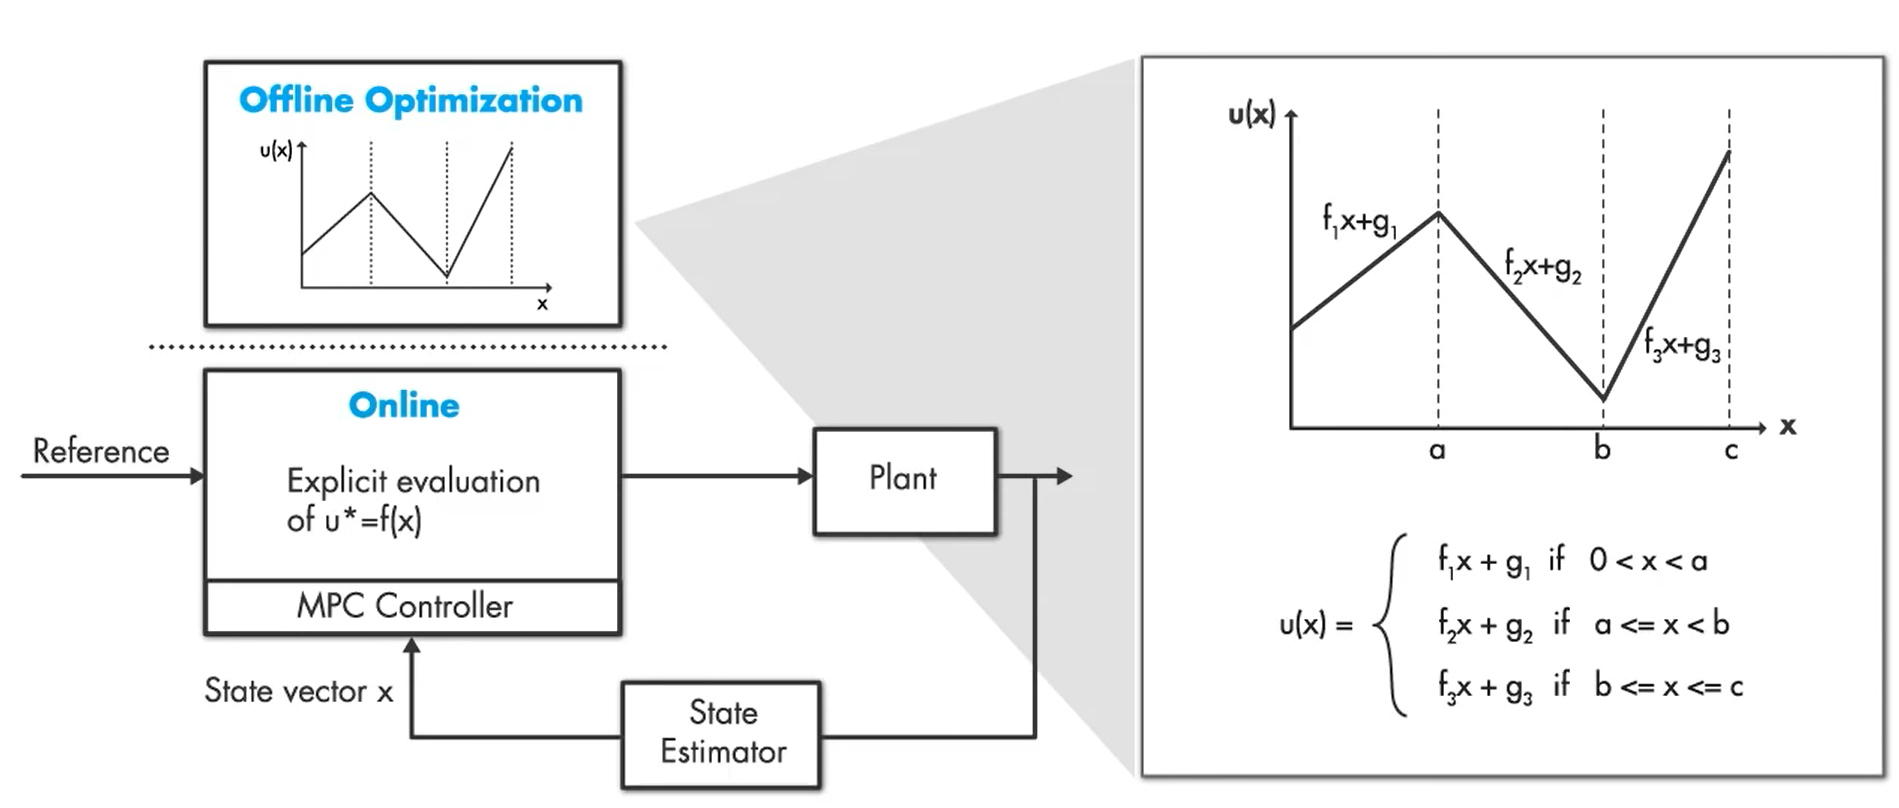
\includegraphics[width=0.9\textwidth]{Images/Control/Explicit_MPC_a}
\caption{Example of an Explicit MPC controller applied on a one-dimensional system \cite{MathWorks2018_new}.}
\label{Explicit_MPC_1D}
\end{figure}

\noindent As can be observed from figure \ref{Explicit_MPC_1D}, the constraints cut the solution space into different regions. And, each region maps into a unique solution.
Another example of an Explicit MPC applied on a two-dimensional system is shown in figure \ref{Explicit_MPC_2D} below. 

\newpage

\begin{figure}[h]
\centering
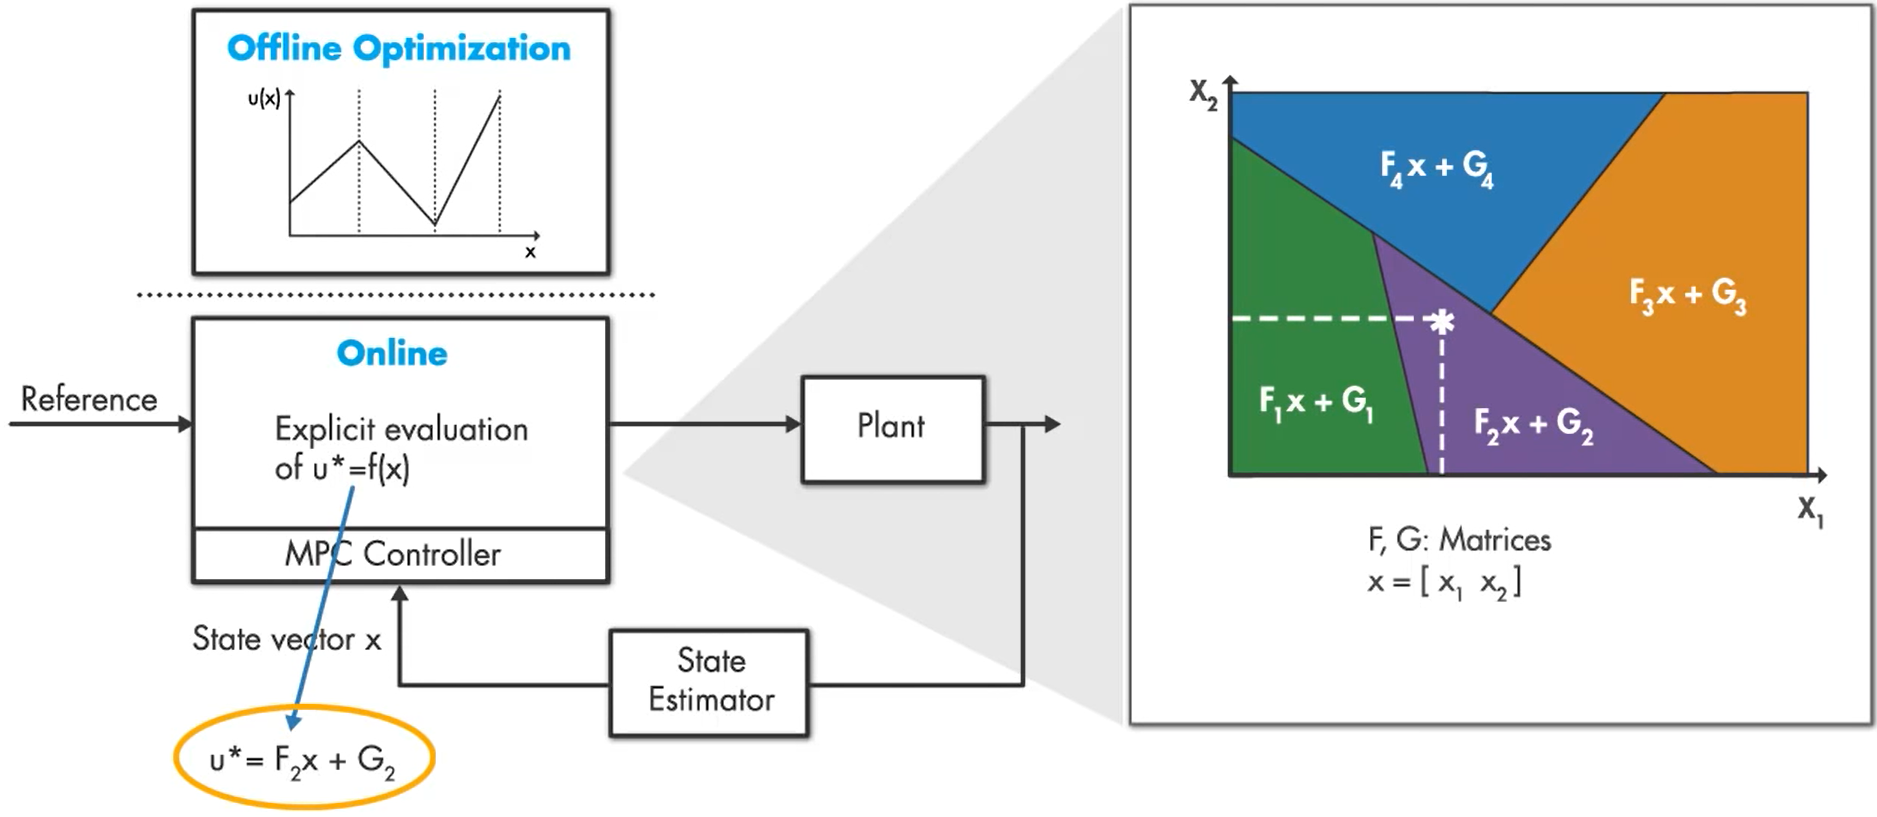
\includegraphics[width=0.9\textwidth]{Images/Control/Explicit_MPC_b}
\caption{Example of an Explicit MPC controller applied on a two-dimensional system \cite{MathWorks2018_new}.}
\label{Explicit_MPC_2D}
\end{figure}

\noindent As can be observed from figure \ref{Explicit_MPC_2D}, the Explicit MPC finds the  region that the current state lies in and evaluates the linear function that creates the current control input.

\noindent Thus, it can be concluded that if the iterative optimization process is reduced to linear function evaluations, then this will greatly simplify the online computations. However, if there is a large number of regions that the state can lie in, then searching for the current state region could sometimes be time consuming. Also, having many regions could cause memory problems for the processor. Thus, the number of regions can be reduced by merging some regions together. However, thee computed solution in that case is not optimal anymore \cite{Hovland2008}.

\paragraph{Suboptimal Solution}
It is another method to improve the computational time of the MPC controller. In a MPC problem, the optimal solution is very unpredictable and can drastically change between each time step. In addition, the computational time may exceed the sample time $T_s$. So, it is mandatory to make sure that a solution can be found within $T_s$ and that there still exists additional time for other tasks that need to be executed \cite{Gulez2014}. A simple example is provided in figure \ref{Suboptimal_solution_example} below where a maximum value for the iterations is determined, and it is taken as 5 for illustration purposes. 


\begin{figure}[h]
\centering
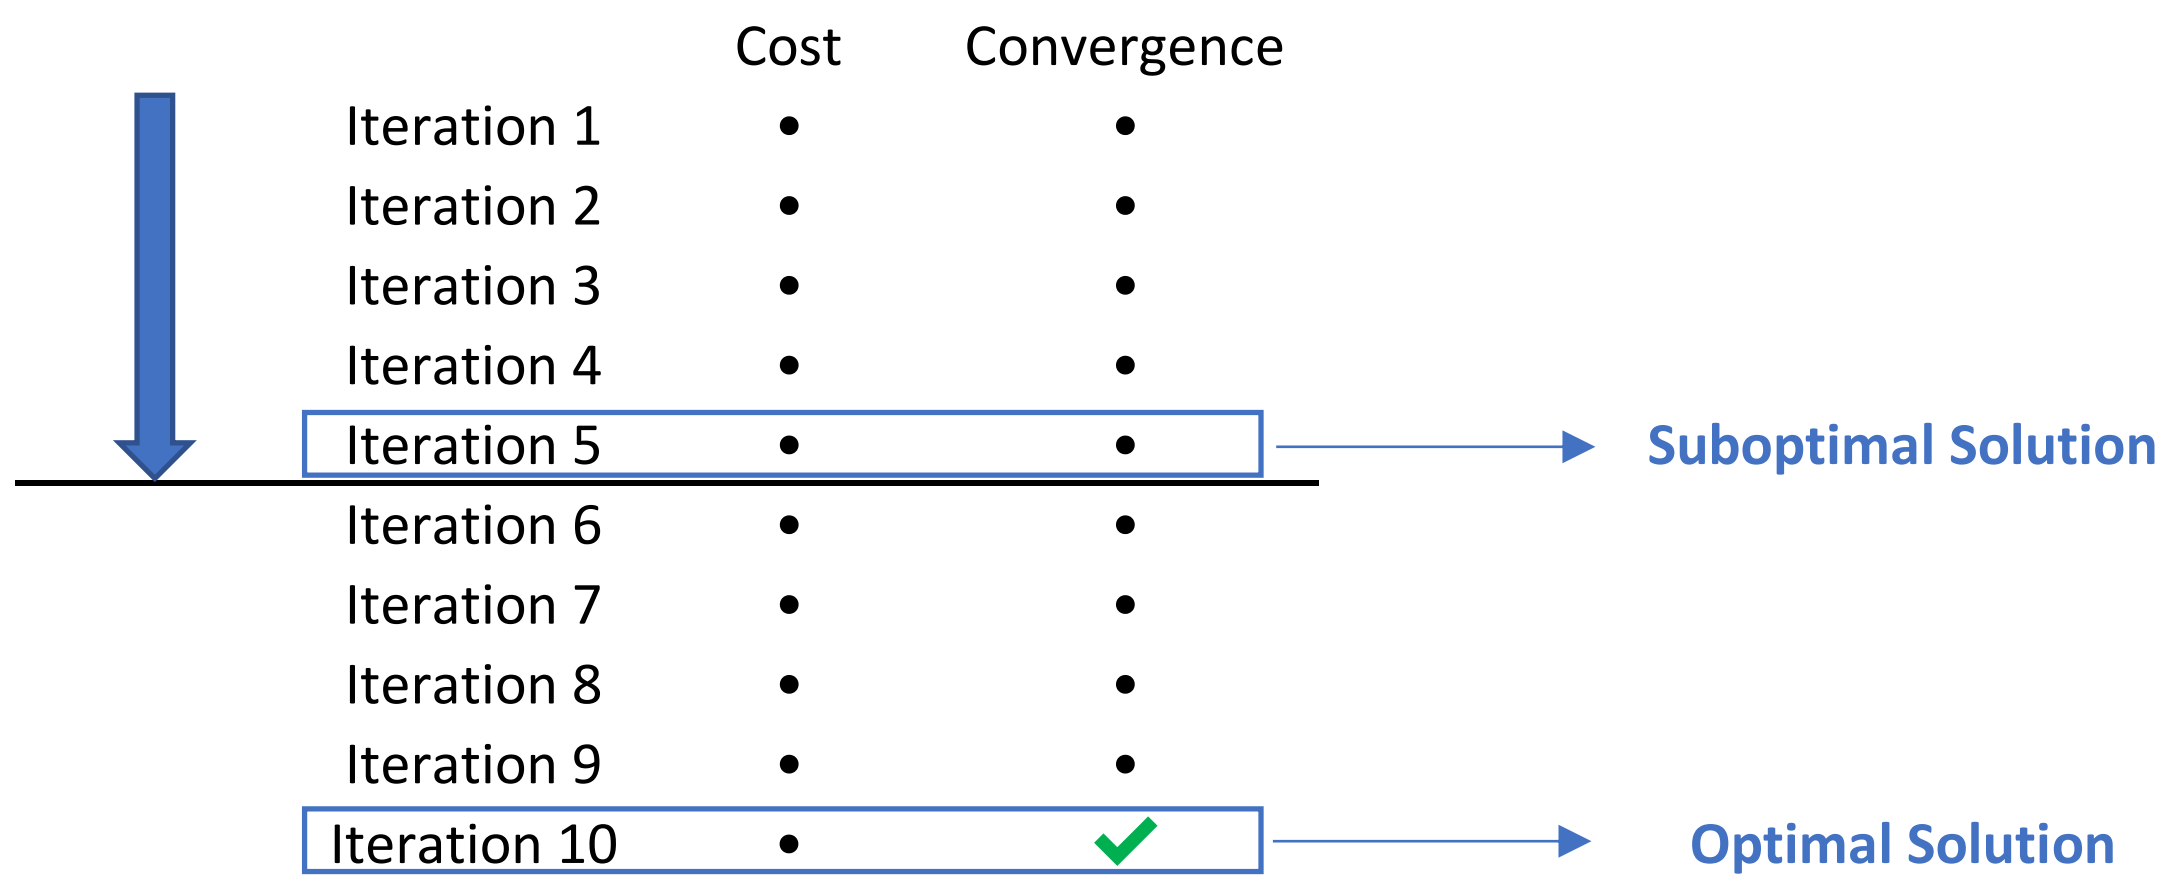
\includegraphics[width=0.8\textwidth]{Images/Control/Suboptimal_Solution.png}
\caption{Example showing how the suboptimal solution is found when the maximum number of iterations is set to 5.}
\label{Suboptimal_solution_example}
\end{figure}

\noindent As can be seen from figure \ref{Suboptimal_solution_example}, the optimal solution is reached in 10 iterations. However, the controller will stop at iteration 5 and take the suboptimal solution. Moreover, it is important to note that the suboptimal solution still satisfies all the constraints of the optimization problem. The only question that remain is how to determine the maximum number of iterations. This can be done by testing the algorithm on the hardware directly and identifying the execution time used by each iteration. Then, the maximum number of iterations is chosen such that the total execution time does not exceed the sample time of the controller.

\subsection{MPC applications on quadrotors}

 There have been numerous applications of MPC on quadrotors. The main MPC applications on drones can be separated into two different categories:

\subsubsection{Centralized MPC}
 
In this type of application, the MPC controller is a signle structure that encapsulates both the translational dynamics and the rotational dynamics. It takes the trajectory waypoints as inputs, and directly outputs the control inputs required to control the quadrotor. This type of implementation of the MPC controller produces the least amount of errors. However, this comes at a cost of a larger computational load.

\begin{figure}[h]
	\centering
	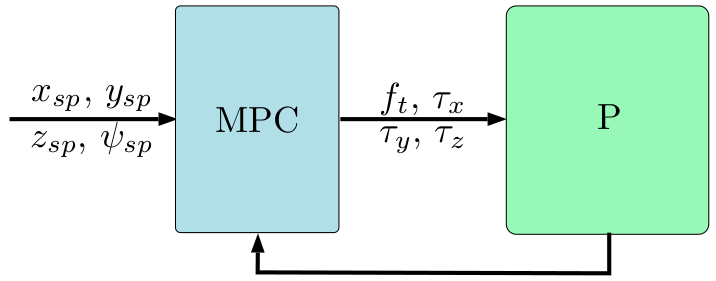
\includegraphics[width=0.7\textwidth]{Images/Control/MPC/centralized_mpc.png}
	\caption{Example of a centralized MPC control loop \cite{Alvarez-Valle2019}.}
	\label{fig:centralized_mpc}
\end{figure}

As can be seen in figure \ref{fig:centralized_mpc}, which represents a centralized control loop structure for a basic MPC, the right block is the plant which represents the quadrotor dynamics. The MPC bloc taks as input the desired trajectory, and outputs control inputs to allow the quadrotor to follow the trajectory.

It should be noted that different versions of the MPC controller shown in figure \ref{fig:centralized_mpc} can exist. For example, another version of the MPC could be that the state variables of roll and pitch angles can be added as outputs. This is mainly implemented in order to ensure that the quadrotor does not take extreme values in roll and pitch angles, which can potentially destabilize it, because no restrictions are being used for these angles otherwise.

\subsubsection{Non-centralized MPC} 

In this type of application, the state-space of the system will be split to obtain two different controllers in a master-slave structure. This more simplified structure allows the implementation of MPC in different embedded systems, each one with less computational load when compared to the complete structure of a centralized MPC. For example, the simplified slave structure can be used to control the attitude of the quadrotor, whereas the master structure can be used to control the position and direction of the quadrotor. In addition, this splitting allows different sample times for the master and slave loops \cite{Bingfang2004}. Furthermore, an implementation of non-centralized MPC could be of having both master and slave structures being MPC controllers. An example of this non-centralized MPC implementation is shown in figure \ref{fig:non_centralized_mpc_1} below:

\begin{figure}[h]
	\centering
	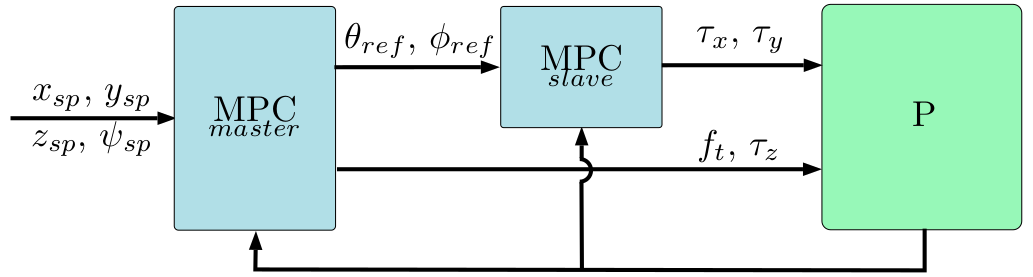
\includegraphics[width=0.9\textwidth]{Images/Control/MPC/non-centralized_mpc_1.png}
	\caption{Example of a non-centralized MPC-MPC control loop \cite{Alvarez-Valle2019}.}
	\label{fig:non_centralized_mpc_1}
\end{figure}

Another implementation is using a MPC controller for the master structure and pairing it with the slave structure that is using a controller with a different control law, such as a PD-P controller, in order to further reduce the computational load. An example of this non-centralized MPC implementation is shown in figure \ref{fig:non_centralized_mpc_2} below:

\begin{figure}[h]
	\centering
	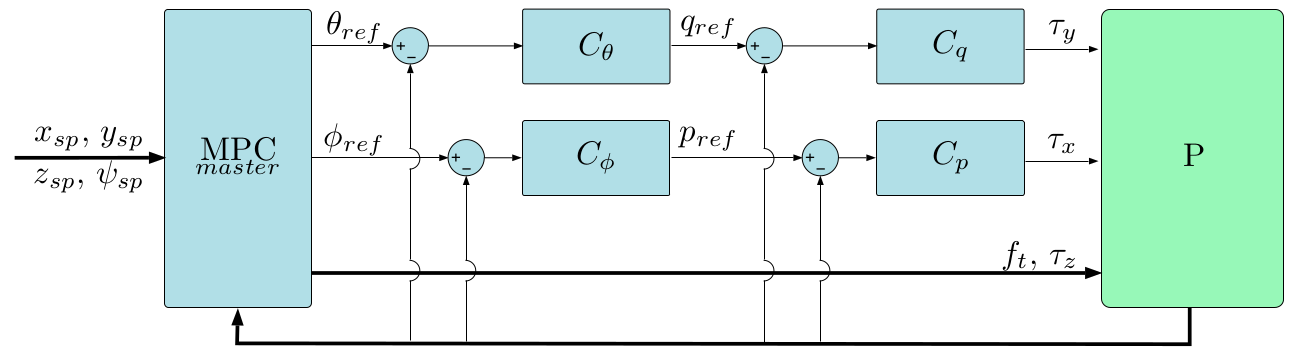
\includegraphics[width=0.9\textwidth]{Images/Control/MPC/non-centralized_mpc_2.png}
	\caption{Example of a non-centralized MPC-PD-P control loop \cite{Alvarez-Valle2019}.}
	\label{fig:non_centralized_mpc_2}
\end{figure}

However, since the control law in this master thesis will be entirely focused on MPC controllers, and since the task will be to follow aggressive trajectories in real-time, then using a non-centralized MPC is a good method to consider, since this will result in a lower computational load on the processor. In other words, it is preferable to follow a trajectory with slightly less accuracy if it results in a faster computation time, which is crucially needed in real-time experimentation.

In the next section, the software used to implement the MPC controller is presented.

 \newpage  
	 

 
 \section{acados – fast embedded optimal control solvers}
 
 \subsection{The difference between acados and other embedded optimal control solvers}
 A big role in bringing MPC to real-time applications is played by the implementation of efficient embedded optimal control methods. This gave rise to software
packages such as:
    \begin{itemize}
        \item \texttt{MPT}: for explicit MPC \cite{MPT3}.
        \item \texttt{qpOASES}: an active-set solver for quadratic programming \cite{qpOASES}.
        \item \texttt{FORCES}: an interior-point solver for quadratically constrained QP and NLPs with optimal control structure \cite{FORCES}.
        \item \texttt{ACADO Code Generation tool}: for tailored SQP based NMPC solvers \cite{ACADO}.
    \end{itemize}

One challenge in developing software for embedded optimal control lies in the trade-off between flexibility, memory usage and speed. Moreover, many of the software packages mentioned above are based on \textit{automatic code generation}. This allows to have self-contained and efficient routines. However, the size of the problem and the choice of algorithms are usually fixed for one specific optimal control instance, which will result in a loss of flexibility. In addition, generated code is often hard to read, thus hard to debug. Finally, it is hard to predict if an automatic code optimization strategy is beneficial or counterproductive for some types of problems. This means that in some cases, a programmer can create faster and more efficient code.

For these reasons, \texttt{acados} does not rely on automatic code generation to perform linear algebra operations. Instead, the high-performance linear algebra package \texttt{BLASFEO} is used. 

Furthermore, other embedded optimal control softwares use global data in order to not sacrifice execution speed and memory. The resulting codebase is difficult to understand, maintain and extend. However, \texttt{acados} organizes the code in a modular way, with formal interfaces between the different algorithmic components. This makes it easier to interchange solvers, routines and libraries needed for the embedded control algorithm.

Finally, \texttt{acados} uses \texttt{CasADi} modeling language instead of \texttt{Mathematics}, \texttt{sympy} or \texttt{MATLAB Symbolic Toolbox}. Many of these softwares make use of expression trees to represent mathematical funcions, which could lead to a large code size, high memory usage and slow evaluation of high-order derivatives for non-trivial models. Whereas \texttt{CasADi} is based on expression graphs. This usually leads to smaller and faster code which make it more suitable for embedded applications. In addition, it is free and open-source software. In summary, \texttt{acados} offers the following:

\begin{itemize}
	\item It contains efficient optimal control algorithms implemented in C.
	\item It has a modular architecture enabling rapid prototyping of solution algorithms.
	\item It interfaces to \texttt{C++}, \texttt{Python} and \texttt{MATLAB}.
	\item It uses the high-performance linear algebra package \texttt{BLASFEO}.
	\item It is compatible with \texttt{CasADi} expressions.
	\item It is deployable on a variety of embedded devices.
	\item It is a free and open-source software.
\end{itemize}

\subsection{Algorithm components for embedded nonlinear optimal control}

\subsubsection{Nonlinear Optimal Control}

The nonlinear optimal control problems that are typically solved by nonlinear MPC (NMPC) have the following form in continuous-time:

\begin{equation}\label{ocp_continuous_form}
        \begin{aligned}
        \min_{x(\cdot),z(\cdot),u(\cdot)} \quad & \int_{t=0}^{T}{l(x(t), z(t), u(t))dt + M(x(T))}\\
        \textrm{s.t.} \quad & x_0 = \bar{x}_0 \\
            & 0 = f(\dot{x}(t), x(t), z(t), u(t)) \text{\hspace{1cm} }t \in [0,T], \\
            & 0 \geq g(x(t), z(t), u(t)) \text{\hspace{1cm} } t \in [0,T] \\
        \end{aligned}
    \end{equation}
    With: 
    \begin{itemize}
		\item $l$: Lagrange term or running cost.
		\item $M$: Mayer term or terminal cost.        
        \item $x$: differential states with $x \in \mathbb{R}^{n_x}$.
        \item $z$: algebraic variables with $z \in \mathbb{R}^{n_z}$.
        \item $u$: control inputs with $u \in \mathbb{R}^{n_u}$.
        \item $f$: Dynamics (as implicit differential-algebraic equations).
        \item g: Nonlinear path constraints.
    \end{itemize} 
 
\subsubsection{Multiple Shooting Discretization}
In \texttt{acados}, the nonlinear OCP is discretized with a \textbf{multiple shooting} approach. The following elements are introduced:
    \begin{itemize}
        \item Time grid: $[t_0, t_1, \ldots, t_N]$ with $t_k < t_{k+1},\text{\space} k = 0, \ldots, N-1$
        \item Discretized state variables: $x_0, x_1, \ldots, x_N$
        \item Algebraic variables $z_0, z_1, \ldots, z_{N-1}$
        \item Controls $u_0, u_1, \ldots, u_{N-1}$ $\Rightarrow$ piecewise constant parametrization is used.    
    \end{itemize}    

The numerical simulation routine on each time interval $[t_k, t_{k+1})$ can be written as:
    $$ \begin{bmatrix}
        x_{k+1}\\
        z_k\\
    \end{bmatrix} = \phi_k(x_k, u_k), \text{\space \space \space} k=0,1, \ldots, N-1$$   
 
By performing multiple shooting discretization on the continuous-time optimal control problem formulation in equation (\ref{ocp_continuous_form}), this will result in the formulation of the nonlinear program (NLP) as shown below.

\newpage

\subsubsection{General Form of the Resulting Nonlinear Program}

The general form of the resulting nonlinear program that can be handled by \texttt{acados} is:

The resulting (general form) NLP problem becomes:
    \begin{equation}\label{NLP}
        \begin{aligned}
        \min_{\substack{x_0,\ldots,x_N\\ u_0,\ldots, u_{N-1} \\ z_0,\ldots, z_{N-1}\\  s_0, \ldots, s_N}} \quad & \sum_{k=0}^{N-1}{l_k(x_k, u_k, z_k) + M(x_N) + \sum_{k=0}^N \rho_k(s_k)}\\
        \textrm{s.t.} \quad & \begin{bmatrix}
                                x_{k+1}\\
                                z_k\\
                                \end{bmatrix} = \phi_k(x_k, u_k) \text{ \hspace{2cm}} k=0,1, \ldots, N-1, \\
                            & 0 \geq g_k(x_k, z_k, u_k) - J_{s,k}s_k \text{\hspace{1.15cm}} k=0,1, \ldots, N-1, \\
                            & 0 \geq g_N(x_N) - J_{s,N}s_N, \\
                            & 0 \leq s_k \text{\hspace{4.6cm}} k=0,1, \ldots, N-1.
        \end{aligned}
    \end{equation}
    
    
    It should be noted that that (\ref{NLP}) includes slack variables $s_k$ which can be reformulated as control inputs $u_k$. This allows the use of \textit{soft} constraints. 
But, the slack variables $s_k$ cannot be included in the dynamics of the system. And, can only enter the cost linearly and quadratically, using the following function:

\begin{equation}
	\rho_k(s_k) = \sum_{i=1}^{n_{s_k}} \alpha_k^i s_k^i + \beta_k^i s_k^{i^2}
\end{equation}

with $\alpha_k^i \in \mathbb{R}, \beta_k^i > 0$. Slack variables $s_k$ can also be used to model piecewise quadratic, and possibly asymmetric cost functions.
    
In addition, \texttt{acados} is capable of exploiting the structure of the widely used linear and nonlinear least-squares functions, and can also handle general nonlinear functions.
    
Moreover, within the constraint function $g_k$ in (\ref{NLP}), \texttt{acados} is able to consider: 

\begin{itemize}
	\item Simple bounds on $x_k$ and $u_k$.
	\item Linear constraints on $x_k$ and $u_k$.
	\item Nonlinear constraints on $x_k$ and $u_k$.
\end{itemize}
    
So, $g_k$ could be formulated as follows:

\begin{equation}
        g_k(x_k, z_k, u_k) = \begin{bmatrix}
            J_{bx,k}x_k \\
            J_{bu,k}u_k \\
            C_{x,k}x_k + C_{u,k}u_k \\
            g_{nonl}(x_k, z_k, u_k) \\
        \end{bmatrix}
    \end{equation}
    where $J_{bx,k}$ and $J_{bu,k}$ are selection matrices that determine which components of $x_k$ and $u_k$ have simple bounds.

The NLP in (\ref{NLP}) can be solved by any general-purpose NLP solver, like \texttt{IPOPT} \cite{IPOPT}. But, \texttt{acados} will use embedded optimal control methods to solve the NLP which are better suited in a real-time setting.

\newpage

\subsubsection{Sequential Quadratic Programming and Real-Time Iterations}

    An embedded SQP algorithm must feature: 
    \begin{itemize}
        \item Numerical integration of the continuous-time dynamics.
        \item Generation of first-order and possibly second-order sensitivities of objective and constraints.
        \item A procedure for approximating the Hessian matrix.
        \item An efficient QP solver.
        \item Initialization strategies for warm-starting the algorithm for the next iteration.
    \end{itemize}

Moreover, the SQP algorithm in acados has the following form:

\begin{align}
	 w^{[i+1]} &=w^{[i]} + \Delta w^{QP}\\
     \pi^{[i+1]} &= \pi^{QP} \\
     \lambda^{[i+1]} &= \lambda^{QP}
\end{align}


Where:
\begin{itemize}
    \item $ w^{[i]} = [x_0^{[i] \intercal}, \ldots, u_0^{[i] \intercal}, \ldots, x_N^{[i] \intercal}]^{\intercal}$ is the primal iterate at SQP iteration $i$.
    \item $\pi^i$ and $\lambda^i$ are the dual iterates, readily available from the QP solution.
\end{itemize}

It should be noted that the algebraic variables are eliminated from the OCP, but numerical approximations of these values are accessible from the numerical integration routine.

Furthermore, the step $\Delta w^{QP}$ is computed by solving the following QP: 
    \begin{equation}\label{step_QP}
        \begin{aligned}
        \min_{\substack{\Delta x_0,\ldots,\Delta x_N\\ \Delta u_0,\ldots, \Delta u_{N-1} \\ \Delta s_o,\ldots, \Delta s_N }} \quad & \sum_{k=0}^{N-1}{  \begin{bmatrix} \Delta x_k \\ \Delta u_k \end{bmatrix}^{\intercal} \overbrace{\begin{bmatrix} Q_k & S_k^{\intercal} \\ S_k & R_k \end{bmatrix}}^{H_k} \begin{bmatrix} \Delta x_k \\ \Delta u_k \end{bmatrix} + \begin{bmatrix} q_k \\ r_k \end{bmatrix}^{\intercal} \begin{bmatrix} \Delta x_k \\ \Delta u_k \end{bmatrix}} \\ & + \Delta x_N^{\intercal} Q_N \Delta x_N + q_N^{\intercal} \Delta x_n \\ & + \sum_{k=0}^N s_k^{\intercal} P_k s_k + p_k^{\intercal} s_k \\
        \textrm{s.t.} \quad & \Delta x_{k+1} = A_k \Delta x_k + B_k \Delta u_k + \phi_k^x - x_{k+1},  k=0,1, \ldots, N-1,\\
            & \Delta x_0 = \bar{x}_0 - x_0 \\
            & -g_k \geq G_k^x \Delta x_k + G_k^u \Delta u_k + s_k, \text{\space \space \space} k=0,1, \ldots, N-1, \\
            & -g_N \geq g_N^x \Delta x_N + s_N, \\
            & 0 \leq s_k, \text{\space \space \space} k=0,1, \ldots, N.
        \end{aligned}
    \end{equation}

\newpage

\subsubsection{Numerical Integration and Sensitivities}

In the family of single step integration methods, there are: 
    \begin{itemize}
        \item \textbf{Explicit} methods: Easy to implement, they rely on a direct combination of explicit evaluations of the right-hand side of the system dynamics. Example: Runge-Kutta method of order 4.
        \item \textbf{Implicit} methods: More complex, it results in a nonlinear system which generally needs to be solved numerically using an iterative procedure such as a Newton-type method. And, when compared to explicit methods, implicit methods have improved numerical stability properties and higher order accuracy.
    \end{itemize}


When using numerical integration methods within direct multiple shooting, the first (and possibly second) order deriatives of the simulation
results with respect to the state and control input values also need to be computed:
    $$ \frac{\partial \phi_k^x (x_k, u_k)}{\partial x_k}, \frac{\partial \phi_k^x (x_k, u_k)}{\partial u_k}, \sum_{i=1}^{n_x} \pi_{k,i} \frac{\partial^2 \phi_{k,i}^x (x_k, u_k)}{\partial^2 (x_k, u_k)} $$
    where $\pi_k \in \mathbb{R}^{n_x}$ is called the \textit{seed vector} \cite{acados2019}, for which the Lagrange multipliers are used to compute the exact Hessian of the Lagrangian.

\subsubsection{Convex Hessian Approximation Methods}

    \paragraph{Gauss-Newton Hessian approximation} In the case of a least-squares objective in (\ref{NLP}):
    \begin{itemize}
        \item $l(x_k, u_k) = \|r(x_k, u_k) \|_2^2, \text{\space \space \space} k=0, \ldots, N-1$
        \item $M(x_N) = \|r_N (x_N)\|_2^2$,
    \end{itemize}
    with $r$: $\mathbb{R}^{n_x} \times \mathbb{R}^{n_u} \Rightarrow \mathbb{R}^{n_r}$, $r_N$: $\mathbb{R}^{n_x} \Rightarrow \mathbb{R}^{n_{r_N}}$

This kind of residual function is a common case in embedded optimization.

The Gauss-Newton Hessian approximation amounts to \cite{acados2019}:
	\begin{equation}
		H^{GN} = blkdiag(H_0^{GN}, \ldots, H_N^{GN})
	\end{equation}	    
    at the linearization point $w^{[i]\intercal} = [x_0^{[i]\intercal}, \ldots, u_0^{[i] \intercal}, \ldots, x_N^{[i] \intercal}]^{\intercal}$, where the Hessian blocks are defined as:
    \begin{align}
    	H_k^{GN} &= \bigg( \frac{\partial r}{\partial (x,u)} (x_k^i, u_k^i) \bigg)^{\intercal} \bigg( \frac{\partial r}{\partial (x,u)} (x_k^i, u_k^i) \bigg), \text{\space \space \space} k=0,\ldots,N-1 \\
    	H_N^{GN} &= \bigg( \frac{\partial r_N}{\partial x} (x_N^i) \bigg)^{\intercal} \bigg( \frac{\partial r_N}{\partial x} (x_N^i) \bigg)
    \end{align}
    
Moreover, the Gauss-Newton Hessian approximation offers a competitive alternative to SQP with exact Hessians, but it only converges linearly. And, for a quadratic objective function in (\ref{NLP}), the same quadratic objective arises in (\ref{step_QP}), and no additional computations are needed.

There exist other Hessian approximation methods in \texttt{acados} and interested readers are referred to \cite{acados2019} for the full description of the other methods.

\subsubsection{Structure-exploiting embedded QP solvers}

There exist different strategies to solve for QP (\ref{step_QP}) in \texttt{acados} \cite{acados2019}:

	\begin{itemize}
        \item \textbf{Sparse approach}: OCP (\ref{step_QP}) can be solved directly by using a general-purpose sparse QP solver. 
        \begin{itemize}
            \item Example: OOQP(primal-dual interior point solver), OSQP(first order method).
        \end{itemize}
        \item \textbf{Structured approach}: OCP (\ref{step_QP}) can be solved by exploiting its multi-stage structure, but dense linear algebra is used. 
        \begin{itemize}
            \item Example: HPMPC, HPIPM (interior-point solvers).
        \end{itemize}
        \item \textbf{Condensing approach}: It uses the dynamics to eliminate the states from the decision variables.
        \begin{itemize}
            \item The state variables are expressed as an explicit function of the current state and future control inputs.
            \item A smaller QP is then obtained with only the control inputs and (possibly) the initial state as optimization variables.
        \end{itemize}
        \item \textbf{Partial condensing approach}: It is a mix between structured and condensing, but only per blocks of $N/N_2$ (with $N$ an integer multiple of $N_2$), and $N_2$ the new horizon length of the partially condensed problem.
        \begin{itemize}
            \item This approach allows finding a better trade-off between horizon length and number of optimization variables for a given problem.
        \end{itemize}
    \end{itemize}

\subsubsection{Real-time iterations}

A downside of \texttt{acados} is that the length of control horizon $m$ cannot be set. In other words, after setting the length the prediction horizon $N$, the control horizon $m$ will directly take the same length as $N$ and it cannot be set to have a different length than $N$. As mention earlier in subsection (\ref{design_parameters}), this could result in significant computational loads.

However, in a real-time control setting, the environment is continuously changing, and it is often sufficient to solve NLP (\ref{NLP}) approximately. In other words, it is useless to have a solution with high accuracy if the computation time deadline has passed.

An existing online method for this approach is the \textit{real-time iteration} (RTI) scheme \cite{Diehl2002}. It allows to solve an inequality-constrained QP in each iteration. The resulting generalized predictor is better suited for predictions across active-set changes, than for example a tangential predictor  acquired from an interior-point method \cite{acados2019}.

 In each RTI, one full iteration of an SQP-type scheme is performed, including generation of the sensitivities with respect to all variables. 
 
 This approach made it possible to implement \texttt{acados} in real-time experiments as shown in \cite{carlos_sartor_zanelli_frison_burgard_diehl_oriolo_2020}
 and \cite{kloeser_schoels_sartor_zanelli_prison_diehl_2020}.
 
 \newpage
 
 \subsubsection{Python Interface Overview}
 
 Before testing the mpc controller in ROS2 and Gazebo, the mpc controller was first designed using the acados Python interface. And, simulations were done by making use of a Runge-Kutta of order 4 integrator that is already implemented in acados. 
 
 
 \begin{figure}[h]
 	\centering
 	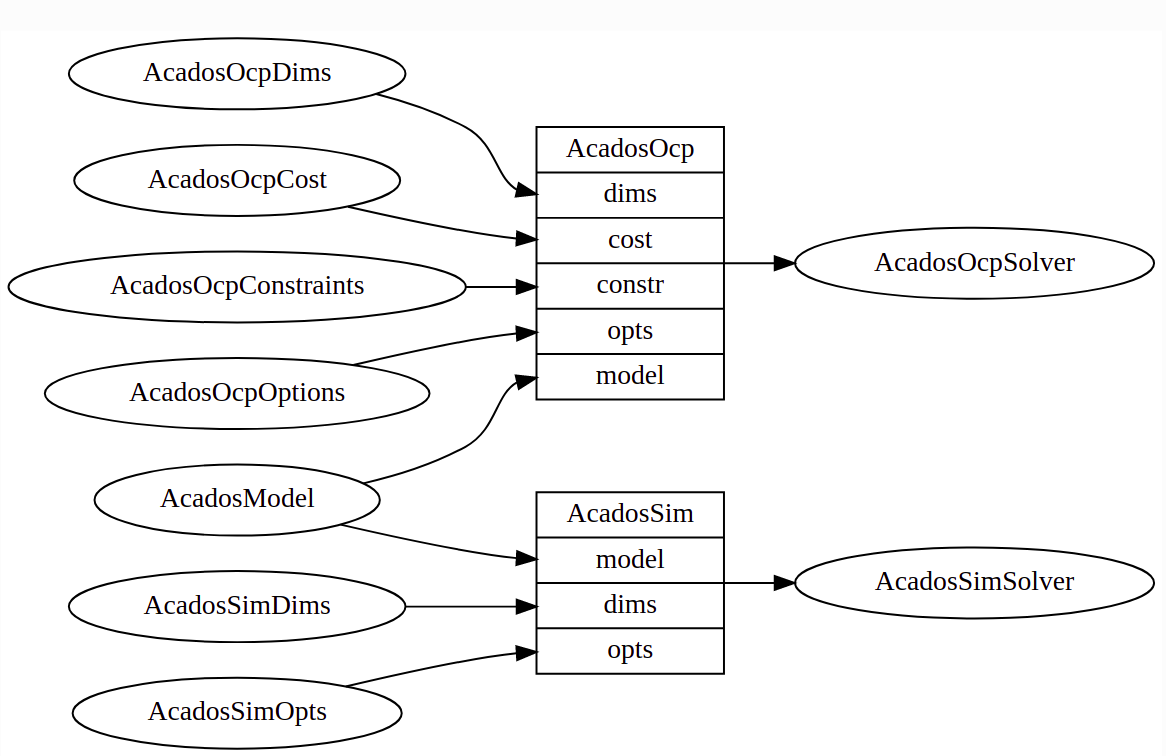
\includegraphics[width=\textwidth]{Images/acados/python_interface.png}
 	\caption{Overview of the Python API classes in acados \cite{Verschueren2018}}
 	\label{fig:python_interface}
 \end{figure}
 
 As can be seen from figure \ref{fig:python_interface}, there exists two main classes in the acados python interface. Namely, \texttt{AcadosOcpSolver} and \texttt{AcadosSimSolver}. 
 
 In order to create the optimal control problem solver class (\texttt{AcadosOcpSolver}), the dynamic model of the system, along with the dimensions of the OCP, the cost function, the constraints and the solver options must be clearly defined. Then, the OCP is solved, which results in the control inputs.
 Then, a simulator class can be used in order to apply the resulting control inputs on the dynamics and compute the new state of the system. So, in order to create the \texttt{AcadosSimSolver} class, the dynamic model of the system must also be used, along with the dimensions and the solver options.
 
 
 
 
 
 
 
\newpage

\section{Flip maneuvers with quadrotors}


The aim of this section is to explain the physics of the flip maneuver, in addition to the major difficulties that relate to the implementation of flipping maneuvers with quadrotors. Furthermore, a review of the existing limitations that the current approaches have are shown and the existing scientific literature is presented. The content of this chapter were thoroughly covered by the previous master students Marco Orsingher \cite{Orsingher2019} and Antonio Marino \cite{Marino2020} for which their papers were used as references for this section.  

\subsection{Physics of a quadrotor flip}\label{multiflip_physics}


In order to perform the tedious process of multi-flip maneuvers with a quadrotor, high angular velocity and large angle attitude control are needed. More conventionally, the multi-flip trajectory can be expressed as a rotation of $2n \pi$ about a flipping axis \textbf{a}, with n the number of desired flips to be carried out by the quadrotor. Physically, the maneuver can be divided into 4 different phases, which are shown in figure \ref{flipping_physics}.

\begin{itemize}
\setlength{\itemindent}{-.5in}
	\item [] \textbf{Climb phase} The quadrotor must accelerate in a vertical direction as much as possible. This will ensure that the required height to perform the multi-flip maneuver is achieved. In fact, while performing the multi-flip maneuver, the thrust forces cannot balance out the weight of the drone. This will cause the drone to start falling. The duration of this phase is based on the number of flips that must be performed by the quadrotor. This number will be chosen by the user.

	\item[] \textbf{Multi-flip phase} This stage begins the moment the vehicle starts rotating and continues until the flipping angle reaches the chosen value of $2n \pi$. In this phase, the quadrotor hits the maximum altitude because of the required high angular velocity and starts falling because of the gravity effect. Generally, all the focus is on following the desired closed-loop attitude, and the vertical position is not controlled. the time spent in this phase depends on the desired number of flips $n$ and on the maximum angular velocity achievable by the quadrotor.
	
	\item [] \textbf{Descent phase} In order for the quadrotor not to crash into the ground, the main idea is to set the maximum thrust reference to the actuation system. This will balance out the gravity force. The higher the number of required flips, the faster the quadrotor will fall due to gravity effects. Thus, this phase ends when the descent is fully balanced out. The user may also decide what the duration of this phase is if the physics of the problem allow a slower descent.
	\item [] \textbf{Re-stabilization phase} In this phase, the altitude of the quadrotor is adjusted to a desired value. Moreover, this phase ends when a new control signal is provided by the user. 
\end{itemize}

\begin{figure}[h]
\centering
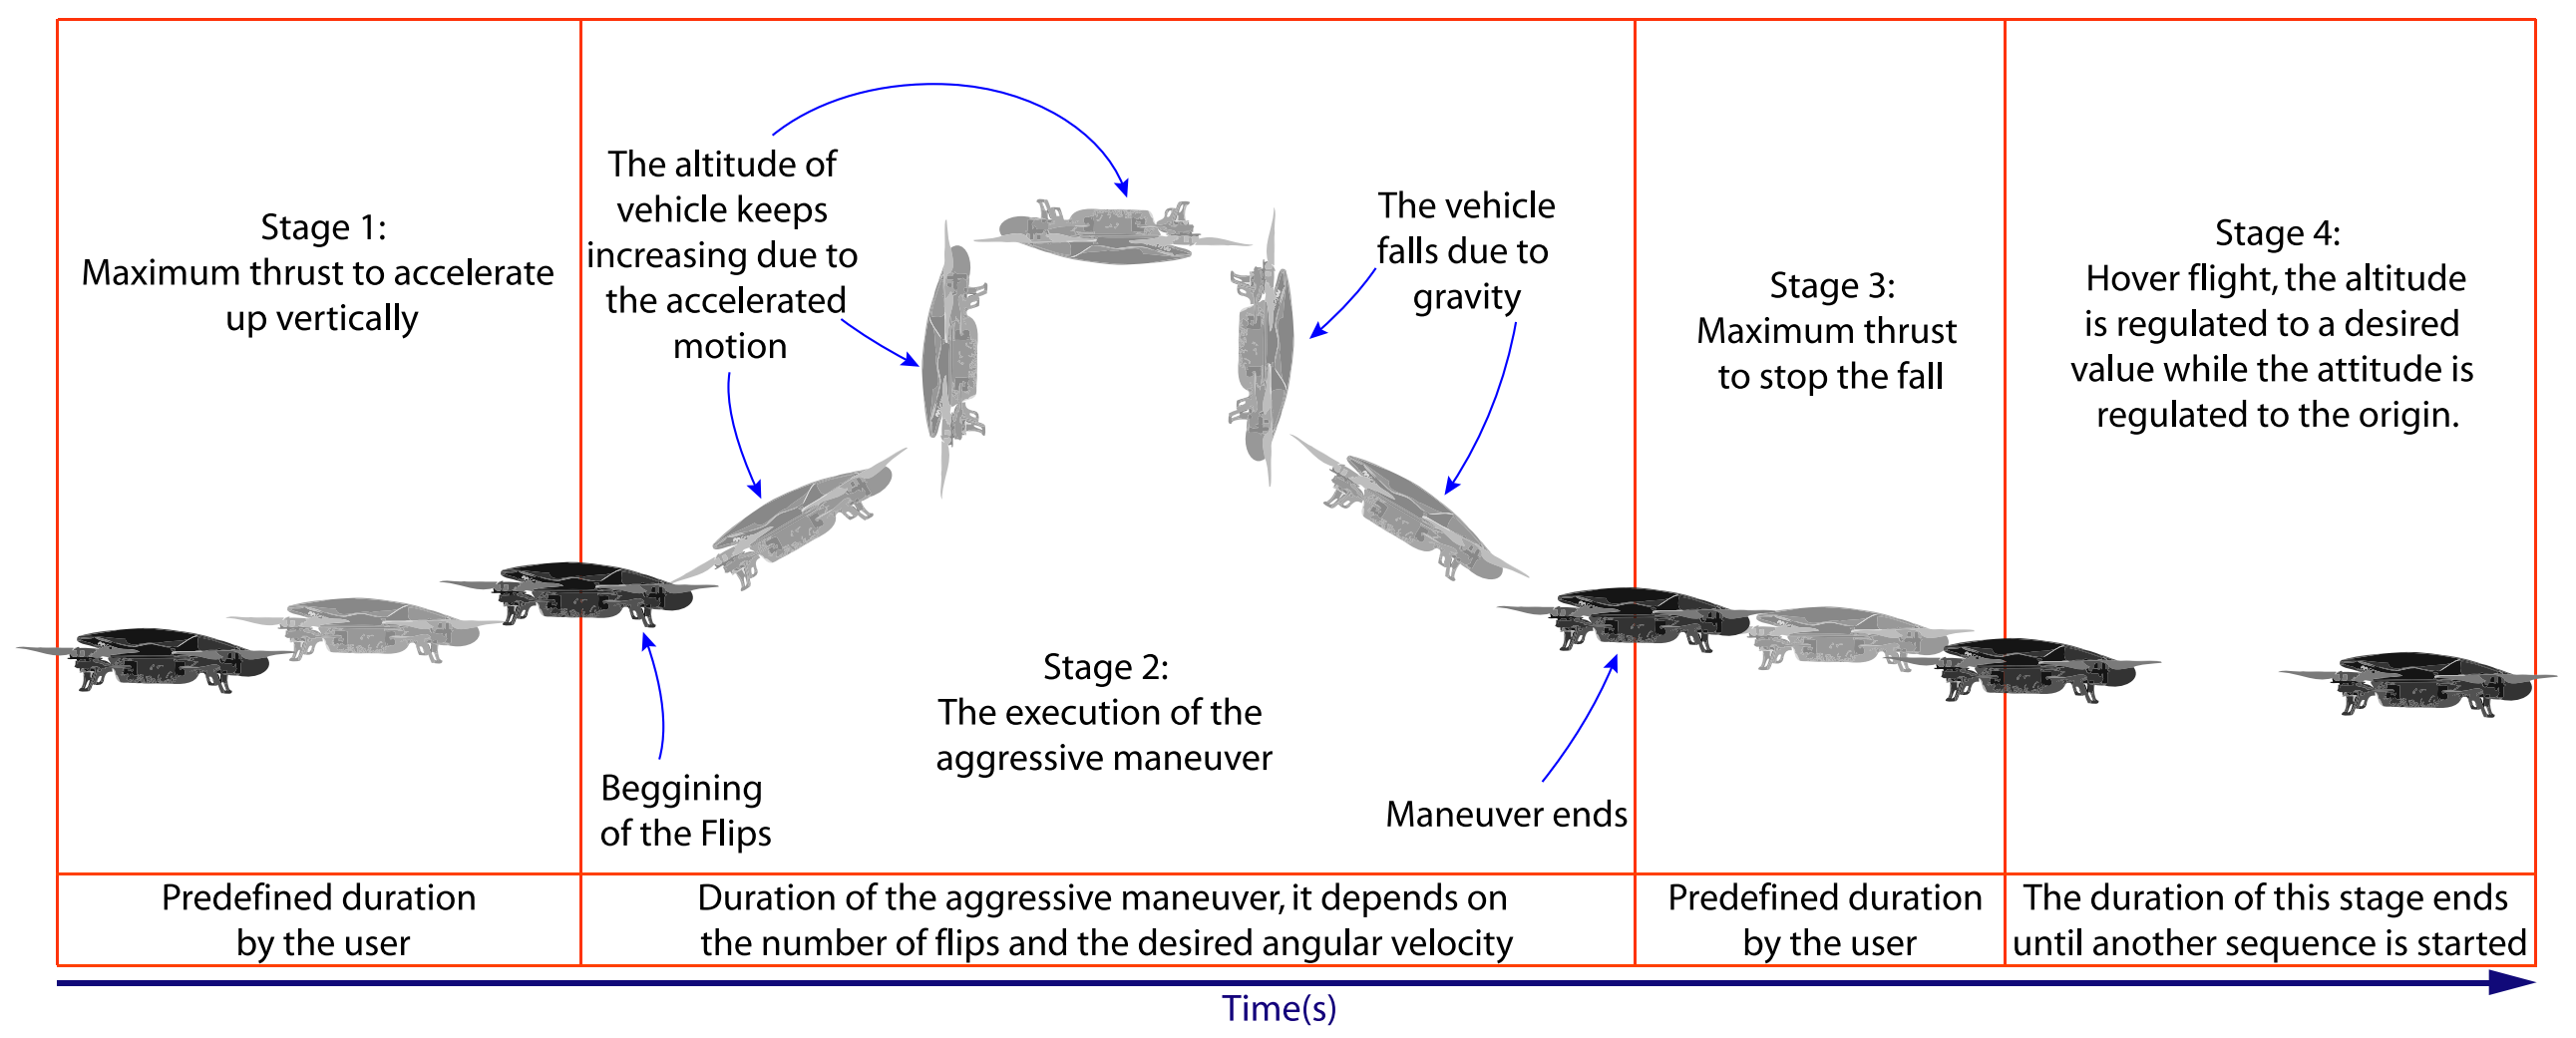
\includegraphics[width=\textwidth]{Images/Flip/Physics}
\caption{Representation of the different phases needed for performing multi-flip maneuvers\cite{Castillo2018}.}
\label{flipping_physics}
\end{figure}
 
 \subsection{Control Approaches for Multi-Flip Maneuvers}
 
The research community has tackled the multi-flip problem numerous times on quadrotors and different methods have been suggested to achieve up to triple flips both indoor and outdoor. The existing research can be stored into three different methods: hybrid systems theory, open-loop iterative learning and closed-loop attitude control. This section gives an inclusive overview and suitable references on the state of the art in flipping maneuvers with quadrotors.
  
 \subsubsection{Hybrid Systems Theory}
 
A convenient approach for dealing with complex systems is to divide them into a set of individual modes. Each mode will have its own continuous dynamics equations. Then, they will be analyzed by using hybrid systems theory. Gillula et al. (\cite{Gillula2011,Gillula2010}) suggested using this strategy for quadrotor multi-flips. The main idea is to breakdown the flipping maneuver into a sequence of individual phases and then use an appropriate technique from hybrid systems theory to generate provable transitions between the modes. By doing this procedure, the maneuver will be able to be performed safely. The separate modes that are considered in this work are shown in figure \ref{hybrid_systems_theory_figure}, which should be right from right to left. When compared to the different phases shown in section \ref{multiflip_physics}, the climb phase is called the \textit{"impulse"}, the multi-flip phase is the \textit{"drift"} and the descent and the re-stabilization phases are merged together and are called \textit{"recovery"}.
 
 \begin{figure}[h]
 \centering
 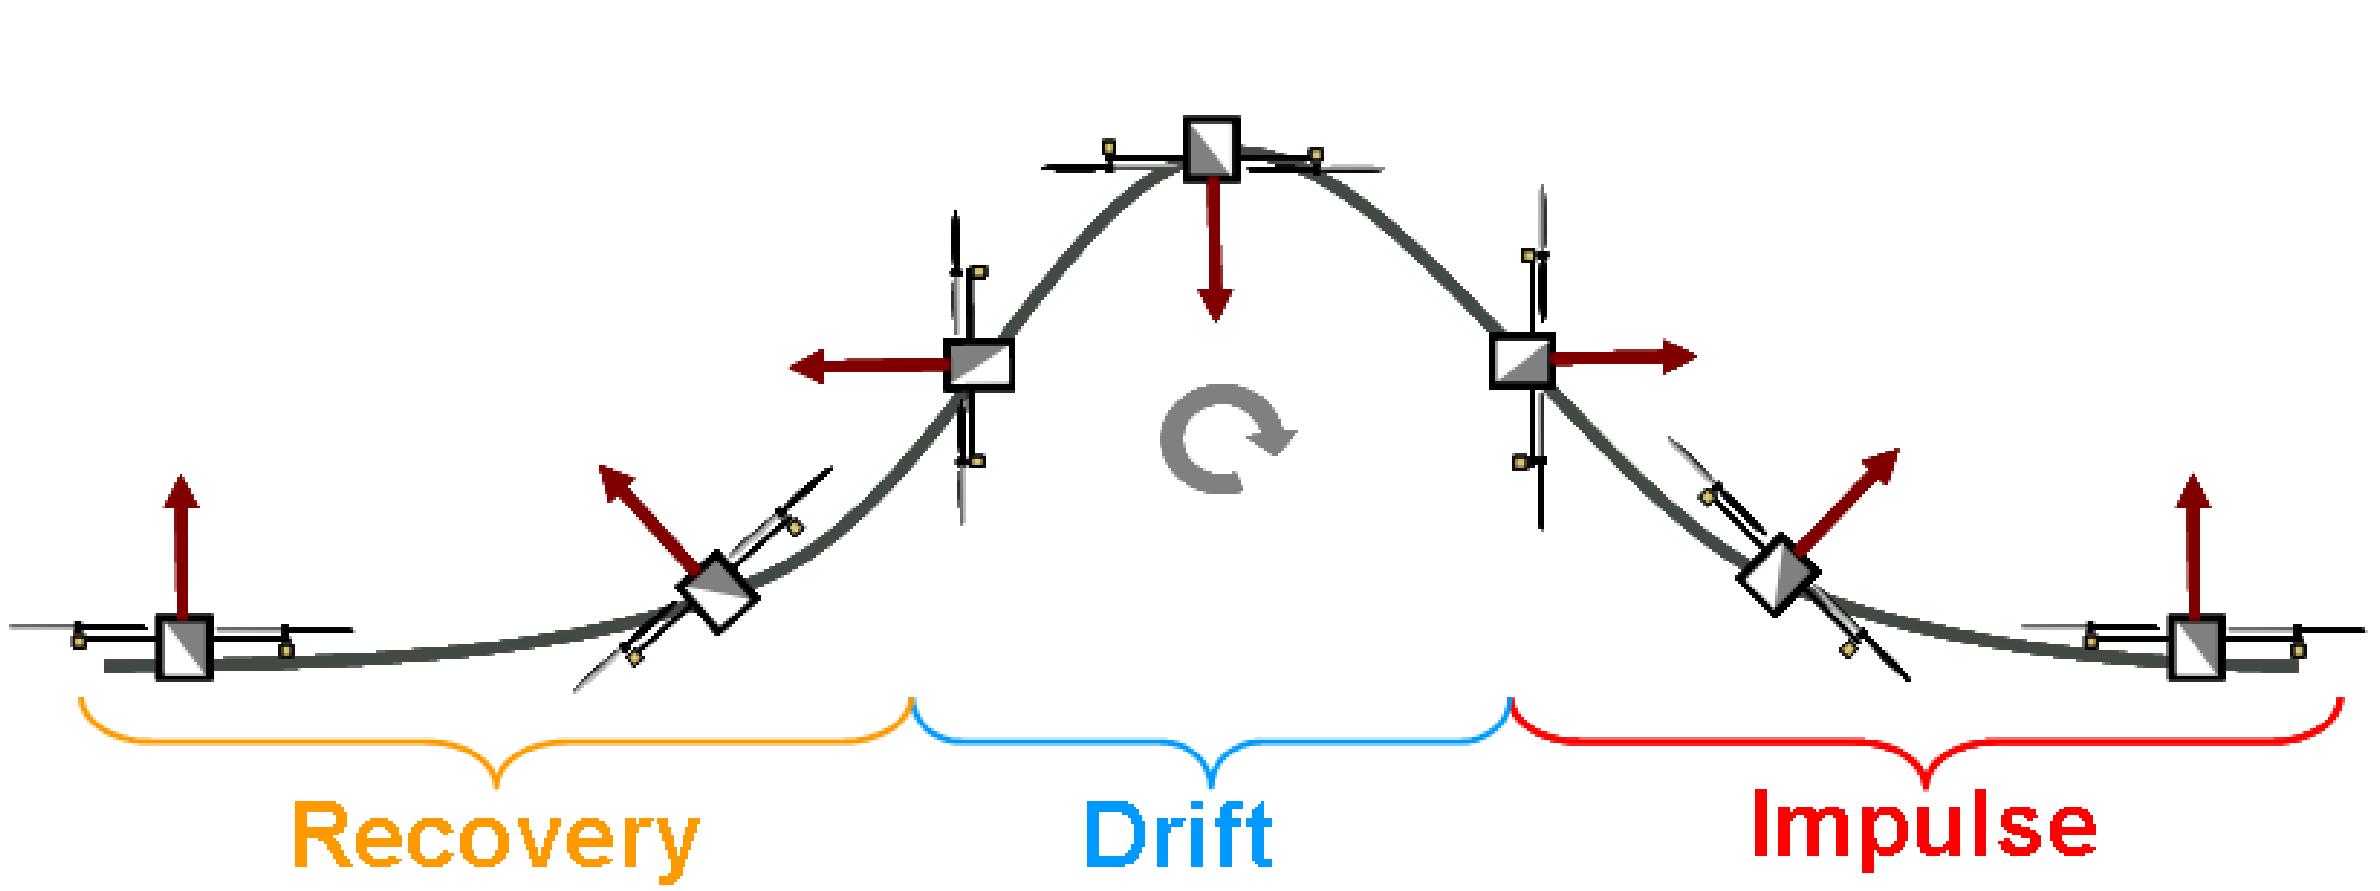
\includegraphics[width=\textwidth]{Images/Flip/Hybrid_Systems_Theory}
 \caption{Representation of the individual phases during a backlip (from right to left)\cite{Gillula2011}}
 \label{hybrid_systems_theory_figure}
 \end{figure}

\newpage
 
 \noindent The tool used for generating feasible transitions between the individual modes is called the \textit{"theory of reachable sets"}. By considering a system characterized by the following dynamics: 

\begin{equation}
	\dot{\textbf{\textsc{x}}}=  \textbf{\textsc{f}} ( \textbf{\textsc{x}}, \textbf{\textsc{u}}, \textbf{\textsc{d}})
\end{equation}


with $\textbf{\textsc{x}}$ the state of the system, $\textbf{\textsc{u}} \in U$ the control input of the system and $\textbf{\textsc{d}} \in D$ a bounded noise applied on the system. In that case, two different types of reachable sets are established:

\begin{enumerate}
	\item A \textit{capture set} which represents all the states for which, for any possible value of the noise $\textbf{\textsc{d}}$, the control input $\textbf{\textsc{u}}$ is still capable of driving the state into a desired state region in a finite time horizon $t$.
	\item An \textit{avoid set} which represents all the states for which, for any possible value of the control input $\textbf{\textsc{u}}$, the noise $\textbf{\textsc{d}}$ will drive the system into an undesired set. Thus, the roles of $\textbf{\textsc{u}}$ and $\textbf{\textsc{d}}$ are reversed when compared to the capture set.
\end{enumerate}

\noindent Generating quadrotor maneuvers using reachable sets is achievable by using a backward approach. The main idea consists of starting from the final desired set, the dynamics of the $n$-th mode can be run in reverse to build a capture set for that phase. This capture set becomes the target region for the $(n-1)$-th node and the procedure will be repeated between every 2 modes. By applying this procedure, feasible transitions between a chain of individual modes can be built. From a mathematical perspective, the problem is formulated as a differential battle between the control and the noise.
In fact, the aim of the control input $\textbf{\textsc{u}}$ is to keep the state of the system away from the region of undesired sets which the noise $\textbf{\textsc{d}}$ is attempting to drive the state of system into (\textit{avoid set}) and also to reach a desired set. Whereas the noise attempts to drive the state of the system out of it (\textit{capture set}). This method has been proven to be successful with a 1.1 kg quadrotor which was able to perform a backflip outdoors. However, the main disadvantage of this method is that it necessitates a long procedure of generating such capture sets and avoid sets. 
 
 \subsubsection{Open-Loop Iterative Learning}

One of the main issues that is related to performing aggressive maneuvers with quadrotors is that having an exact physical modeling of the quadrotor during an intense flight procedure is very complicated. In addition, generating reference trajectories for aerobatic flight is not an easy operation. Beginning from these factors, Lupashin et al. (\cite{Lupashin2010,Lupashin2011,Lupashin2012})
designed a simple open-loop iterative learning method to perform multi-flip maneuvers without performing any aerodynamic modeling nor trajectory planning. The workflow of this method is shown in figure \ref{Open_Loop_iterative_Learning} on the left.



\begin{figure}[h]
     \centering
     \begin{subfigure}[b]{0.45\textwidth}
         \centering
         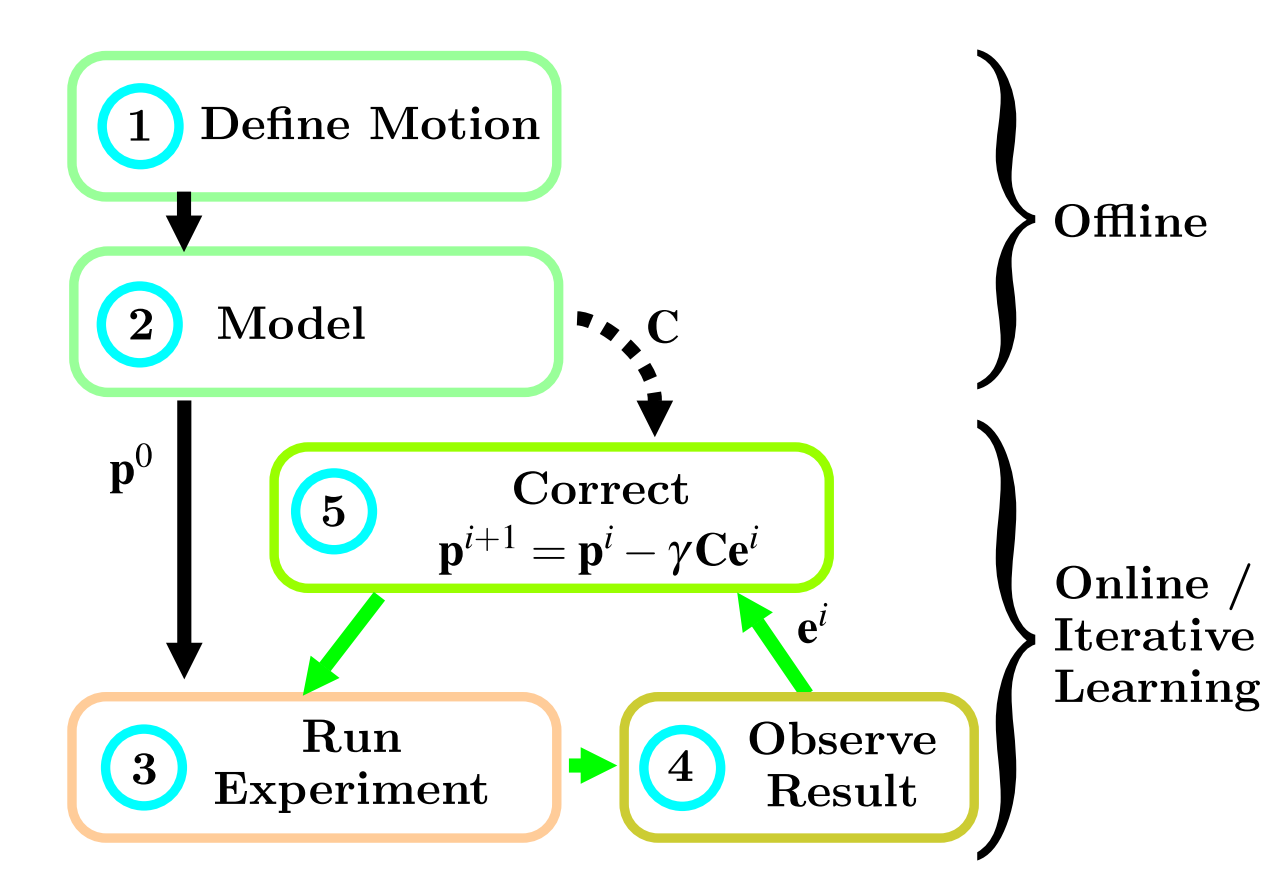
\includegraphics[width=\textwidth]{Images/Flip/Open_Loop_iterative_learning_a}
         \caption{The global workflow of the algorithm}
         \label{fig:Open_Loop_a}
     \end{subfigure}
     \hfill
     \begin{subfigure}[b]{0.45\textwidth}
         \centering
         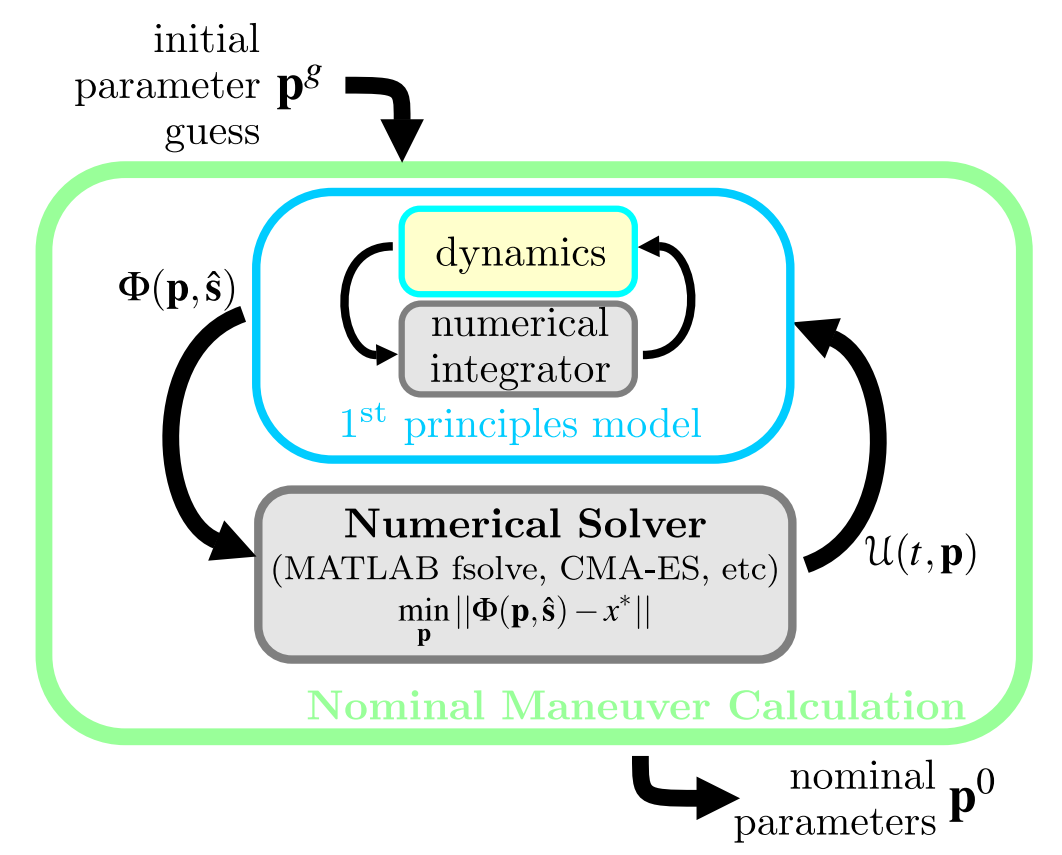
\includegraphics[width=\textwidth]{Images/Flip/Open_Loop_iterative_learning_b}
         \caption{The global workflow of the algorithm}
         \label{fig:Open_Loop_b}
     \end{subfigure}
        \caption{The open-loop iterative learning workflow for performing multi-flips with quadrotors\cite{Lupashin2012}.}
        \label{Open_Loop_iterative_Learning}
\end{figure}

\noindent The first step which is needed is to determine the desired motion in a parameterized manner, so that it is possible to optimize vector $\textbf{\textsc{p}}$ over such parameters. $\textbf{\textsc{p}}$ contains the time and the accelerations needed during each phase of the flip maneuver.  The second procedure which is needed to initialize the iterative learning algorithm is to calculate the nominal motion and to build the correction matrix. Starting from a simplified model of the quadrotor and a coarse initial guess $\textbf{\textsc{p}}^g$, then a numerical solver is utilized to calculate the nominal parameters $\textbf{\textsc{p}}^0$ in order to execute the multi-flip maneuver. In fact, assuming that the desired final state $\textbf{\textsc{x}}^{*}$ can be attained with the control input $\textbf{\textsc{u}}(\textbf{\textsc{p}},t)$ and by referring to $\bm{\Phi}(\textbf{\textsc{p}},\hat{\textbf{\textsc{s}}})$ as the final state of the nominal system after the maneuver is executed.(with the vector $\hat{\textbf{\textsc{s}}}$ representing physical constants), then the nominal set of parameters $\textbf{\textsc{p}}^0$ is the solution of the following optimization problem, as shown in figure \ref{Open_Loop_iterative_Learning}:

\begin{equation}
	\textbf{\textsc{p}}^0 = \text{arg}\min \|\bm{\Phi}(\textbf{\textsc{p}},\hat{\textbf{\textsc{s}}})-\textbf{\textsc{x}}^{*}\|
\end{equation}


\noindent Moreover, by denoting $\bm{\Phi}(\textbf{\textsc{p}}^0,\hat{\textbf{\textsc{s}}})$ as the final state of the nominal model obtained using the nominal set of parameters calculated earlier, then the correction matrix for the iterative learning algorithm is expressed as follows:

\begin{equation}
	\bm{C}=\bigg(\frac{\partial \bm{\Phi}(\textbf{\textsc{p}}^0,\hat{\textbf{\textsc{s}}})}{\partial \textbf{\textsc{p}}}\bigg)^{-1}
\end{equation}

\noindent In the end, steps 3 to 5 in figure \ref{fig:Open_Loop_a} will then run online in an iterative manner until a proposed convergence criterion is satisfied. For $i=0 \ldots n$, the motion is carried out on the quadrotor itself while using the current set of parameters $\textbf{\textsc{p}}^i$ and the final measured error $\textbf{\textsc{e}}^i$. Subsequently, the parameters are updated according to the following law: 

\begin{equation}
\textbf{\textsc{p}}^{i+1} = \textbf{\textsc{p}}^i - \gamma \textbf{\textsc{C}}\textbf{\textsc{e}}^i
\end{equation}

with $\gamma$ being a step size which is defined by the user. This method is very simple does not require complex computations. But, it is by definition an open-loop method. Thus, there are no guarantees that the maneuver will be performed successfully. In fact, a triple flip maneuver has been done during experiments with this method, however the repeatability of this result is a big problem. In addition, "creating a parameterized input trajectory formulation that results in a robust learning strategy remains a difficult and tedious task" \cite{Lupashin2012}.
 
 
 \subsubsection{Closed-Loop Attitude Control}
 
 The most known strategy for obtaining great results in flipping maneuvers of quadrotors is to use closed-loop control just for the attitude part of the platform, thus the position of the center of mass during the flipping maneuver is ignored. Many research works can be recognized under this context, and all of them follow the same ideology: a proper reference on attitude or angular velocity is planned and then tracked in closed-loop with a nonlinear control law. Each paper is distinguished from the others based on the strategy that is chosen to build the control law: attractive ellipsoid method \cite{Castillo2018}, geometric control \cite{Lee2010},  energy-based control\cite{Badawy2016} , direct Lyapunov method \cite{Wang2014}.
Particularly, Chen et al. (\cite{Chen2016}, \cite{Chen2017} ,\cite{Chen2018}) generated interesting series of papers  within this framework that should be mentioned because they applied the method on the same physical platform of this thesis (Crazyflie 2.0); moreover, significant theoretical contributions have been provided in these papers to greatly comprehend the issue of quadrotor flipping. Particularly, three elements have been investigated:

\begin{enumerate}
	\item A new depiction of the flipping angle, called $\phi_g$, such that a flip around a random axis $\textbf{\textsc{a}}$ through the center of mass of the quadrotor can be determined. This has permitted to execute multiple flips about the body-fixed axis $\textbf{\textsc{b}}_1$, and another general axis, rotated by $45 ^{\circ}$ on the ($\textbf{\textsc{b}}_1$,$\textbf{\textsc{b}}_2$) plane.
	\item A meticulous angular speed planning approach using cubic splines to produce the reference signal $\bm{\omega}_d$ in such a way that the dynamics of actuation are respected by ensuring that $w_{max}$ is never surpassed. Particularly, the reference is made out of three distinct stages, corresponding to the physical stages presented in figure \ref{closed_loop_a}. In fact, throughout the \textit{climb phase} a rising-speed section  $\bm{\omega}_{d,1}$ is needed to reach  $\bm{\omega}_{max}$, then a stage of constant-speed at  $\bm{\omega}_{d,2}= \bm{\omega}_{max}$ is held while the quadrotor is flipping (\textit{multi-flip phase}), and in the end, the angular velocity $\bm{\omega}_{d,3}$ is reduced to zero within the \textit{descent} and \textit{re-stabilization phase}. The use of cubic functions ensures that the angular accelerations is kept continuous during all the process. Other works, such as \cite{Castillo2018}, suggested equivalent shape, however linear functions were used instead of splines. Considering that the time derivative of a linear function is just a constant, this resulted in undesirable jumps in the angular reference.\\
Considering the desired number of rotations accumulated with each stage $\Phi_{g,i}1$, the time of each stage is changed based on the current flipping angle $\phi_g$:

\begin{equation}
	\bm{\omega}_d(t) = \begin{cases}
	\bm{\omega}_{d,1} \text{\hspace{0.5cm} if \hspace{0.5cm}} \phi_g \leq \Phi_{g,1} \\
	\bm{\omega}_{d,2} \text{\hspace{0.5cm} if \hspace{0.5cm}} \Phi_{g,1} < \phi_g \leq \Phi_{g,1} + \Phi_{g,2} \\
	\bm{\omega}_{d,3} \text{\hspace{0.5cm} if \hspace{0.5cm}} \Phi_{g,1} + \Phi_{g,2} < \phi_g \leq \Phi_{g,1} + \Phi_{g,2} + \Phi_{g,3} \\
	\end{cases} 
\end{equation}	

where: 

\begin{equation}
	\Phi_{g,1} + \Phi_{g,2} + \Phi_{g,3} = 2 n \pi 
\end{equation}

in order to carry-out the flip.

\begin{figure}[h]
     \centering
     \begin{subfigure}[b]{0.45\textwidth}
         \centering
         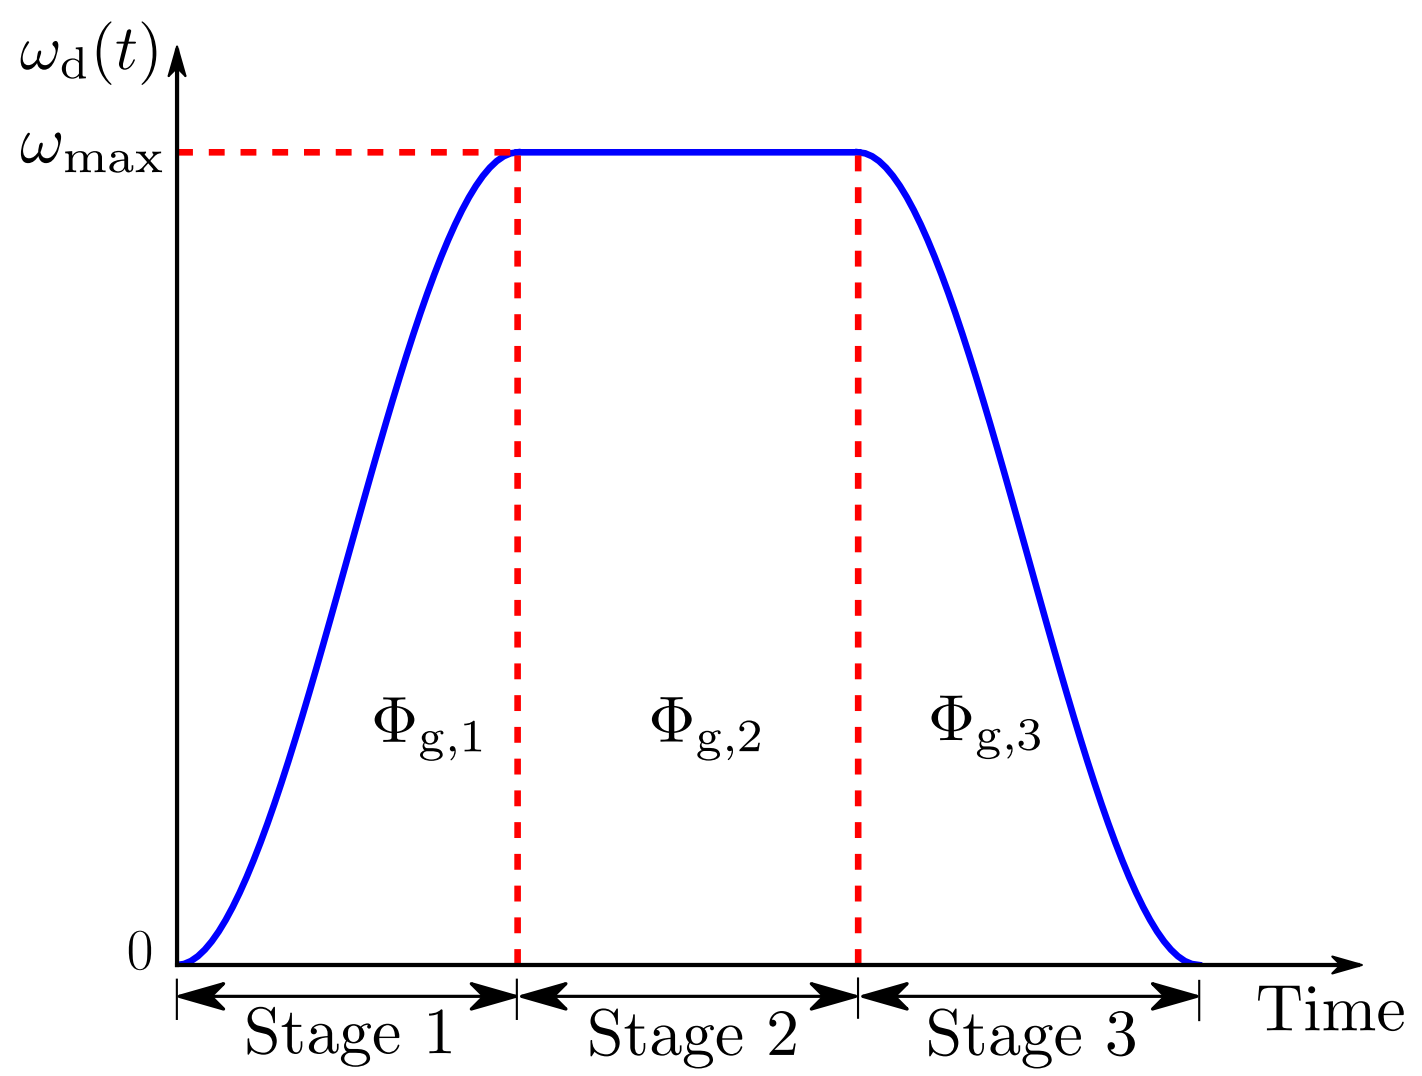
\includegraphics[width=\textwidth]{Images/Flip/Closed_Loop_a}
         \caption{The reference of the angular velocity.}
         \label{closed_loop_a}
     \end{subfigure}
     \hfill
     \begin{subfigure}[b]{0.45\textwidth}
         \centering
         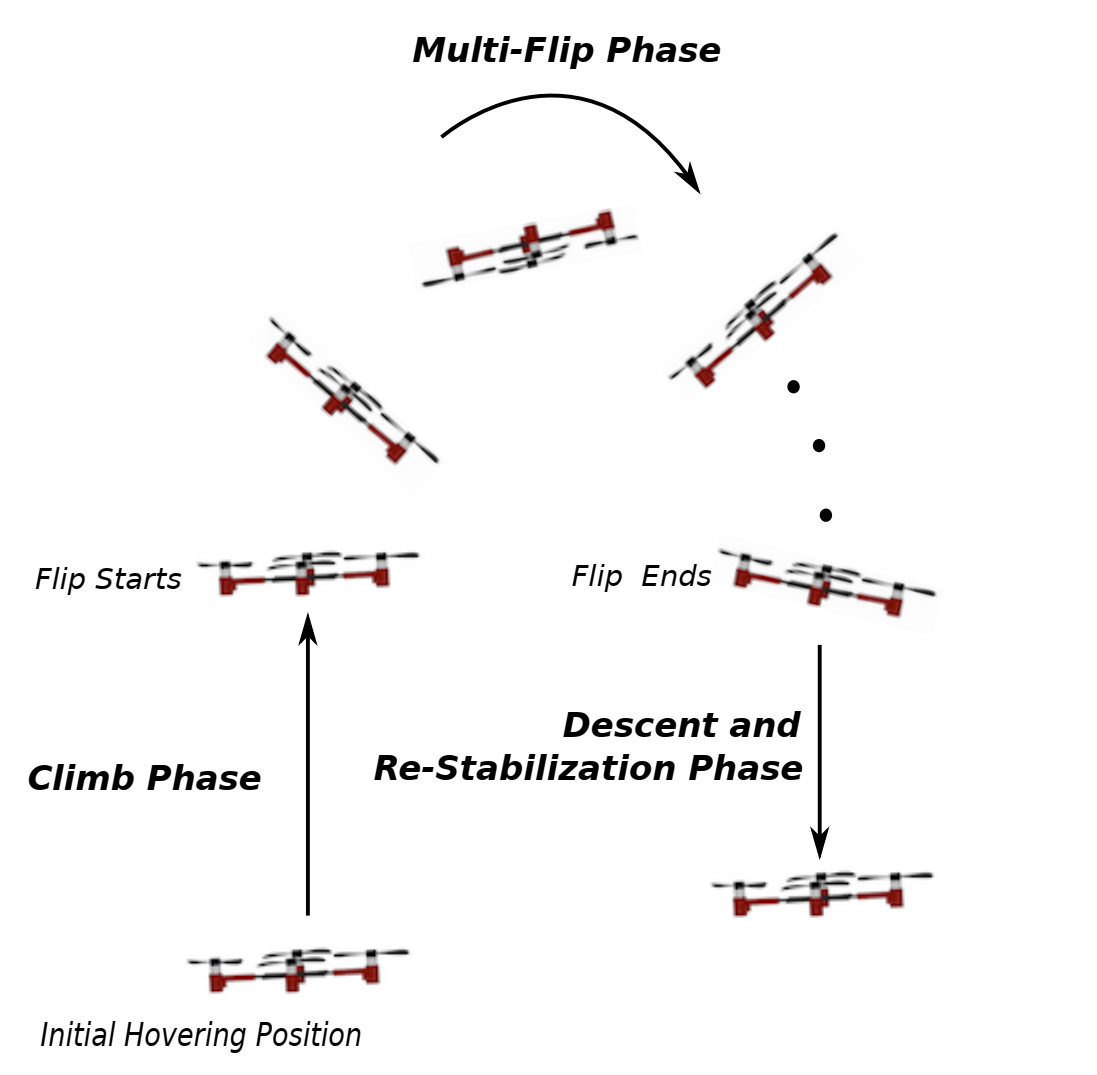
\includegraphics[width=0.8\textwidth]{Images/Flip/Closed_Loop_b}
         \caption{The stages of the multi-flip maneuver.}
         \label{closed_loop_b}
     \end{subfigure}
        \caption{The reference of the flipping speed and the different flipping phases. \cite{Chen2016}}
        \label{closed_loop_c}
\end{figure}

	\item Three distinct control methods to track the reference of the angular speed, which are then compared in terms of the root mean square error. First, a linear time-invariant (LTI) has been proposed \cite{Chen2016} as follows. Provided the error of the angular velocity 
	$\textbf{\textsc{e}}_{\omega} = \bm{\omega} - \omega_d \textbf{\textsc{a}}$ and the error of the angular acceleration $\textbf{\textsc{e}}_{\alpha} = F(s) \bm{\omega} - \dot{\omega}_d \textbf{\textsc{a}}$, with F(s) a filter expressed as $F(s) = \lambda s(s+\lambda)^{-1}$, $\lambda >0$, the consequence control law is: 
	
\begin{equation}
	\bm{\tau} = -\bm{K}_{\omega} \textbf{\textsc{e}}_{\omega} - \bm{K}_{\alpha} \textbf{\textsc{e}}_{\alpha}
\end{equation}

In the subsequent works, a backstepping control approach \cite{Chen2017} has been examined to solve the latency issue which is the result of the slow response of the actuators, in addition to an adaptive control law to estimate unknown parameters on the fly \cite{Chen2018}. In the two cases, these methods achieved better performance when compared to the LTI controller. However, they were not able to successfully reduce the oscillation of the angular velocity within the descent and re-stabilization phase.

\end{enumerate}

\noindent Regardless, this series of papers are by far the most successfull and comprehensive work available in literature on performing multi-flip maneuvers with quadrotors.
 
 
 \subsection{Shortcomings of Current Strategies}
 The control approaches for multi-flip maneuvers that have been presented in section {\ref{control_approaches_for_multi_flip_maneuvers}} demonstrate that the implementation of flipping maneuvers is currently addressed as a more complicated version of the classical attitude control problem. But, no attention has been given on the consequent Cartesian path of the center of mass of the quadrotor, nor on an accurate depiction of the climb phase. In fact, within the first stage, the maximum thrust is established in order to acquire sufficient height. However, none of the works presented above deals with comprehensive altitude analysis in order to give an approximation of the necessary duration for the climb phase. This is mainly done heuristically in experiments. This problem, combined with the fact that the attention is put only on attitude planning and control, results in a totally erratic trajectory for the quadrotor. Thus, it is important to be able to predict the consequent trajectory of the quadrotor during a flipping maneuver. Because, this will help to keep the quadrotor safe, particularly in complex outdoor settings.
 
 
\newpage 
% \chapter{Actual work}
 
% When dealing with rectangled triangles (see Figure \ref{triangle}) I sometimes used this theorem from \cite{pythm001}:
%  \begin{equation}\label{theo}
%   a^2 + b^2 = c^2
%  \end{equation}The demonstration is in Appendix \ref{sec:prooftheorem}. 
%
%  \begin{figure}[h]\centering
%  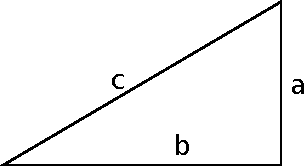
\includegraphics[width=.5\linewidth]{triangle1}
%  \caption{A triangle with letters} \label{triangle}
%  \end{figure}
 
\chapter{MPC Design and Simple Simulations}
In this chapter, the equations of motions of the planar quadrotor and the 3D quadrotor will be presented. And, an extended Kalman filter (EKF) will be designed for the planar case to test the controller in the presence of disturbance. Then, the MPC controller design will be presented. Finally, the MPC controller will by making the quadrotor follow a circular trajectory.

\section{System Modeling} 
In this section, the equations of motion of both the planar quadrotor and the 3D quadrotor will be presented and explained. However, the notion of position and orientation will be explained first. The two main references used for this section are \cite{Fantoni2016} and \cite{Erskine2021}. 

\subsection{Notion of Position and Orientation}

The configuration of a vehicle, namely the \textit{pose}, includes the parameters that pertmits to describe the mobile frame $R_M$ with respect to the working frame $R_O$. In addition, there are several methods to describe the rotation of a rigid body in space, for instance, Euler angles, Cardan angles, \cite{Goldstein1980}, etc. The main distinction between the Euler angles and the Cardan angles is that Cardan angles express rotations around three different axes (e.g. $x-y-z$, or $x-y'' -z''$), whereas Euler angles utilize the same axis for both the first and third elemental rotations(e.g., $z-x-z$, or $z-x'-z''$)

A common representation of the pose of a vehicle in 3D Euclidean space is the following:



\begin{equation}
q=[\begin{array}{c c c c c c }
x & y & z & \psi & \theta & \phi
\end{array}]^{\intercal}
\end{equation}

The pose can be described as the transformation from the working frame related to the environment $R_O$ to the mobile frame $R_M$ based on the four following procedures \cite{Fantoni2016}:

\begin{itemize}
	\item The translation $\overrightarrow{OM}$ from $R_O$ to $R_M$: $(M,\overrightarrow{s_0}, \overrightarrow{n_0}, \overrightarrow{a_0} )$.
	\item The rotation $(\psi, \overrightarrow{a_0})$ where $\psi$ is the yaw angle from $R_O(M,\overrightarrow{s_0}, \overrightarrow{n_0}, \overrightarrow{a_0} )$ to $R_1(M,\overrightarrow{s_1}, \overrightarrow{n_1}, \overrightarrow{a_0} )$.
	\item The rotation $(\theta, \overrightarrow{n_1})$ where $\theta$ is the pitch angle from $R_1$ to $R_2 (M,\overrightarrow{s_2}, \overrightarrow{n_1}, \overrightarrow{a_1} )$.
	\item The rotation $(\phi, \overrightarrow{s_2})$ where $\phi$ is the roll angle from $R_2$ to $R_M (M,\overrightarrow{s_2}, \overrightarrow{n_2}, \overrightarrow{a_2} ) = R_M$ 
\end{itemize}

\begin{figure}[h]
\centering
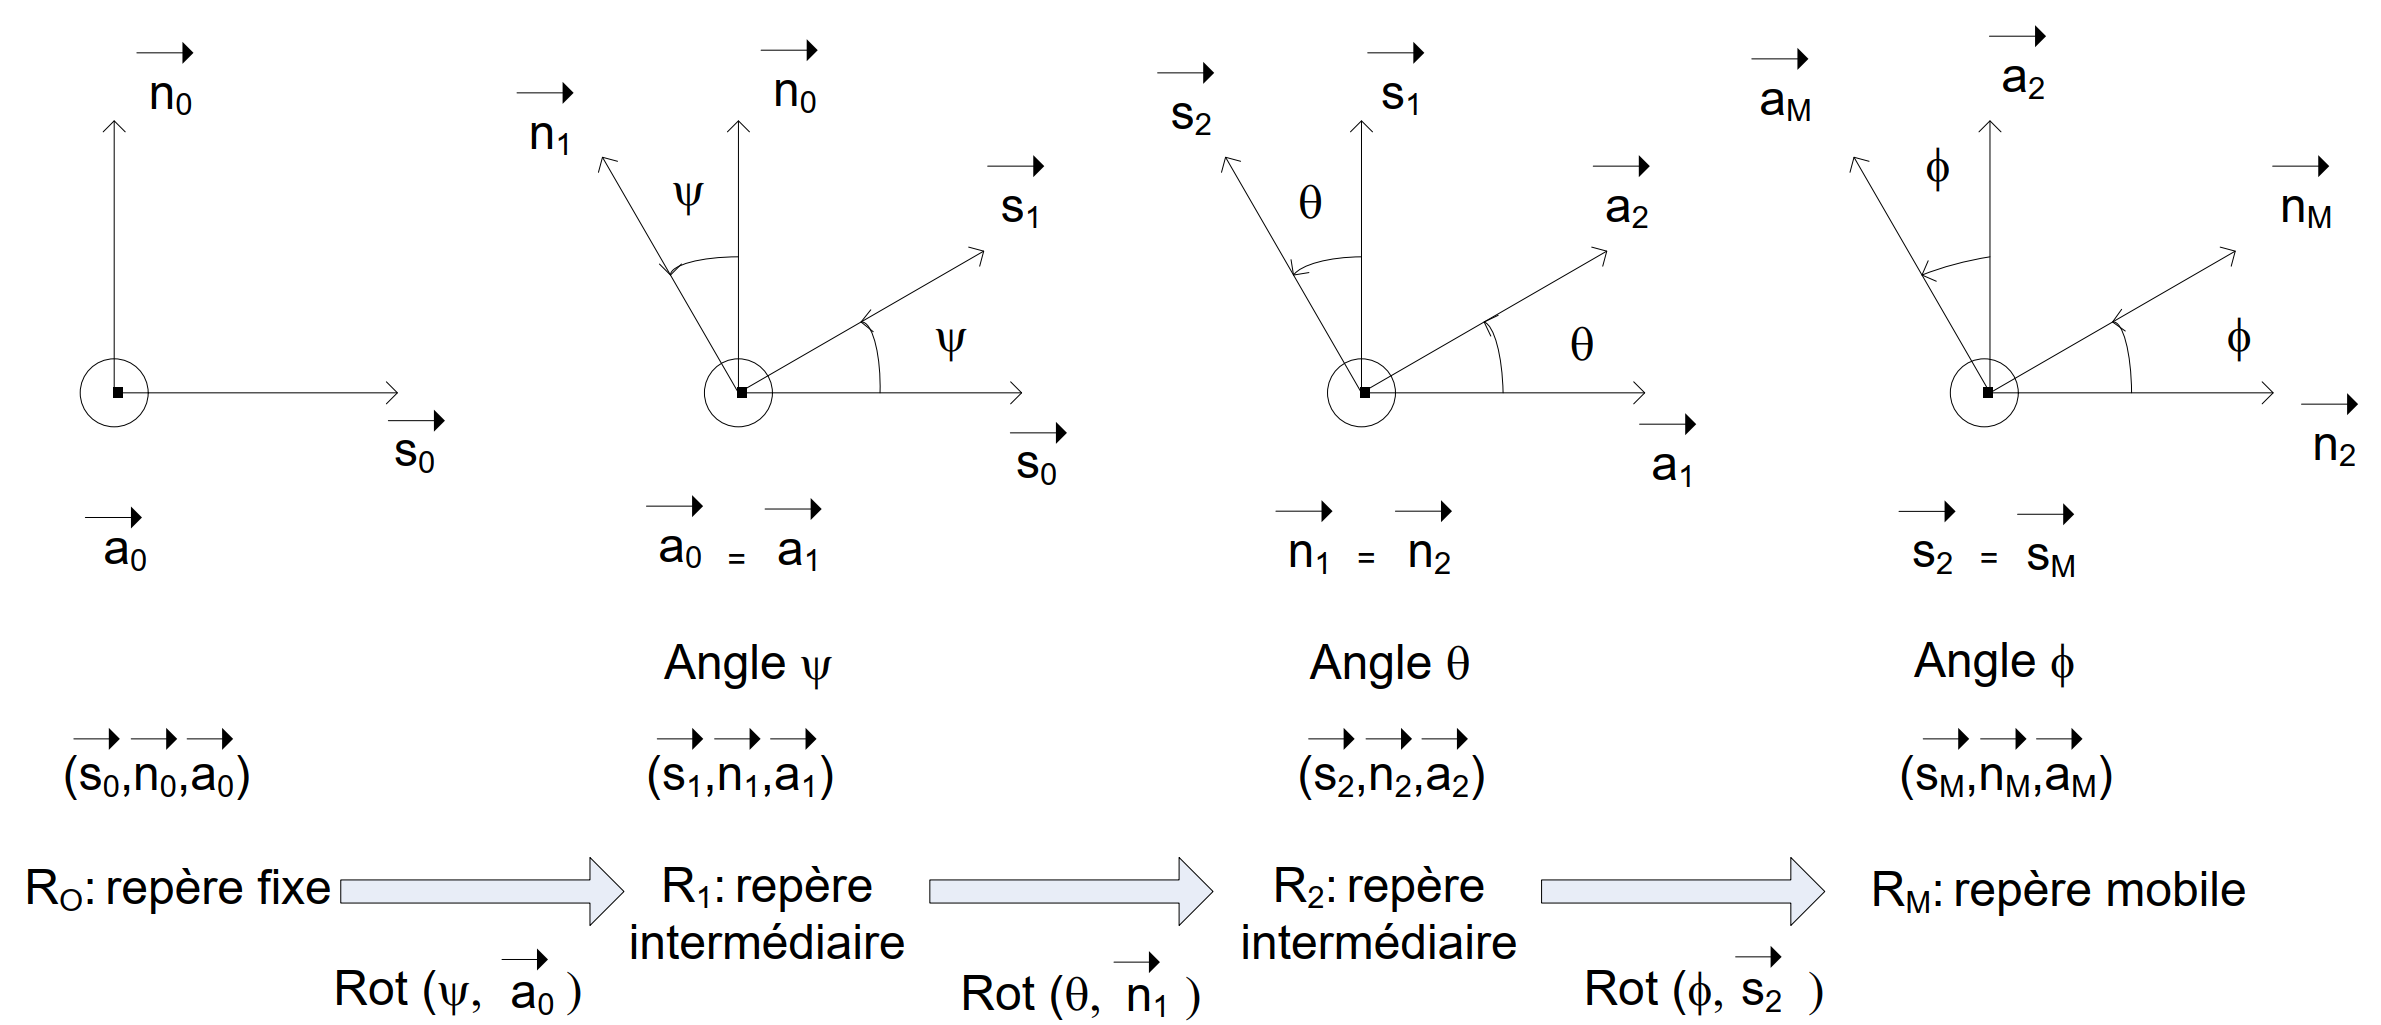
\includegraphics[width=\textwidth]{Images/Modeling/Fantoni_d}
\caption{Representation of the Euler Transformations \cite{Fantoni2016} }
\label{Fantoni_d}
\end{figure}

\newpage

The related change of coordinates matrices are expressed as follows:


\begin{equation}
	L = {}^{O}A_1 = Rot(\psi, \overrightarrow{a_0}) = \begin{bmatrix}
	\cos \psi && - \sin \psi && 0 \\
	\sin \psi && \cos \psi && 0 \\
	0 && 0 && 1 
	\end{bmatrix}
\end{equation}

\begin{equation}
	T = {}^{1}A_2 = Rot(\theta, \overrightarrow{n_1}) = \begin{bmatrix}
	\cos \theta && 0 && \sin \theta \\
	0 && 1 && 0 \\
	- \sin \theta && 0 && \cos \theta 
	\end{bmatrix}
\end{equation}

\begin{equation}
	R = {}^{2}A_M = Rot(\phi, \overrightarrow{s_2}) = \begin{bmatrix}
	1 && 0 && 0 \\
	0 && \cos \phi && - \sin \phi \\
	0 && \sin \phi && \cos \phi 
	\end{bmatrix}
\end{equation}

with $L, T$ and $R$ denoting rotation matrices of roll, pitch and yaw respectively.
Hereafter, $Rot(\psi, \overrightarrow{a_0})$, $Rot(\theta, \overrightarrow{n_1})$ and $Rot(\phi, \overrightarrow{s_2})$ will denote the corresponding change of coordinate matrices.

Thus, the transition matrix from the mobile frame to the fixed frame is then expressed as follows: 

\begin{align}
	LTR &= {}^{O}A_M = Rot(\psi, \overrightarrow{a_0}) Rot(\theta, \overrightarrow{n_1}) Rot(\phi, \overrightarrow{s_2}) \nonumber \\
	&= \begin{bmatrix}
	\cos \psi \cos \theta && - \sin \psi \cos \phi + \cos \psi \sin \theta \sin \phi && \sin \psi \sin \theta + \cos \psi \sin \theta \cos \phi \\
	\cos \theta \sin \psi && \cos \psi \cos \phi + \sin \psi \sin \theta \sin \phi && - \sin \phi \cos \psi + \sin \psi \sin \theta \cos \phi \\
	-\sin \theta && \cos \theta \sin \phi && \cos \theta \cos \phi
	\end{bmatrix}
\end{align}


\subsection{Inputs}

The principal forces and torques that the quadrotor is subject to, are generated by the rotations of the propellers. 

\paragraph{The forces} The forces that are acting on the quadrotor are the weight and the consequent lift which is created by the 4 rotors:

\begin{equation}
\overrightarrow{F_{\xi}}= \overrightarrow{P} + \sum \overrightarrow{f_i}
\end{equation} 

with the weight is expressed as 
$ \overrightarrow{P}= \begin{bmatrix}
0 \\ 
0 \\
-mg \\
\end{bmatrix}$

And, $\overrightarrow{f_{i}}$ is the lift resulting from every individual motor $M_i$ given that the motors $M_1$ and $M_3$ are rotating in the counter-clockwise direction and the motors $M_2$ and $M_4$ are rotating in the clockwise direction. So, $\overrightarrow{f_i}$ is expressed as $\overrightarrow{f_i}=\begin{bmatrix}
0 \\ 
0 \\
f_i \\
\end{bmatrix}=b \begin{bmatrix}
0 \\ 
0 \\
\Omega_i^2 \\
\end{bmatrix} $  

$f_i = b \Omega^2; i=1,\ldots,4$\\
$\Omega_i$: rotational velocity of motor $M_i$\\
$b$: Thrust coefficient\\

The consequent lift is the full thrust of the UAV and is expressed by $u=\sum \overrightarrow{f_i}$. It is lying on the same line as the $u_z$ axis of the $R_U$ frame where the final expression of $\overrightarrow{F_{\xi}}$ is made of two parts . The first part (the weight)  is expressed in the fixed frame and the second part (the total thrust $u$) is expressed in the mobile frame: 

\begin{equation}
\overrightarrow{F_{\xi}}  = \begin{bmatrix}
0 \\
0 \\
-mg \\
\end{bmatrix} 
+ 
b \begin{bmatrix}
0 \\ 
0 \\
\Omega_1^2 + \Omega_2^2 + \Omega_3^2 + \Omega_4^2\\
\end{bmatrix}=
\prescript{O}{}{\begin{bmatrix}
0 \\
0 \\
-mg \\
\end{bmatrix}}
+ b \prescript{U}{}{\begin{bmatrix}
0 \\ 
0 \\
\Omega_1^2 + \Omega_2^2 + \Omega_3^2 + \Omega_4^2\\
\end{bmatrix}}
\end{equation}

\paragraph{The torques}
Regarding the torques, they are also divided into two parts. The first part is the result of the relations between the velocities of the rotors. Whereas the other part is generated by the gyroscopic effects that are resulting from the change of attitude direction of the rotors. In fact, a rotation around the $u_x$ or $u_y$ axis coupled to the rotation of the rotors that is executed around the $u_z$ axis, generates a torque respectively on $u_x$ or $u_y$ axis.

By taking $\tau=\begin{bmatrix}
\tau_1 && \tau_2 && \tau_3 
\end{bmatrix}^{\intercal}$ to be the consequent torque of the quadrotor. It is divided into two parts, namely $\tau_a$ which contains the rotation torques (roll,pitch and yaw) on the 3 axes ($\tau_{\phi}, \tau_{\theta}, \tau_{\psi}$) and the torque $\tau_G$ which is the result of the gyroscopic effects of the rotors, which is usually neglected in many works.

\begin{equation}
	\tau = \tau_a + \tau_G
\end{equation}

with:

\begin{itemize}
	\item $\tau_a = \begin{bmatrix}
\tau_{\phi}\\
\tau_{\theta}\\
\tau_{\psi}\\
\end{bmatrix}= \begin{bmatrix}
l(f_4 - f_2)\\
l(f_3 - f_1)\\
\sum \tau_{M_i}\\
\end{bmatrix}$\\
$\sum \tau_{M_i} = \sum d \Omega_i^2=d(\Omega_1^2-\Omega_2^2+\Omega_3^2-\Omega_4^2); i=1,\ldots 4$: motor torque about the axis.\\
$d$: drag coefficient .\\
$l$: distance between the center of gravity (CoG) of the quadrotor and the axis of motor $M_i$.

	\item $\tau_G=\overrightarrow{\omega}\times J_r \begin{bmatrix}
0 \\
0 \\
\Omega_1 - \Omega_2 + \Omega_3 - \Omega_4 \\
\end{bmatrix} = \begin{bmatrix}
-q J_r (\Omega_1 - \Omega_2 + \Omega_3 - \Omega_4)\\
p J_r (\Omega_1 - \Omega_2 + \Omega_3 - \Omega_4)\\
0 \\
\end{bmatrix}$

$\overrightarrow{\omega} = \begin{bmatrix}
p \\
q \\
r \\
\end{bmatrix}$: angular velocities in the body frame.
$\Omega_i$: spinning speeds of motors $M_i$.
$J_r$: rotor inertia.
\end{itemize}

Thus, the total torque $\bm{\tau}$ is expressed as follows:

\begin{equation}\label{total_torque_equation}
\bm{\tau} = \begin{bmatrix}
\tau_1\\
\tau_2\\
\tau_3\\
\end{bmatrix} = \tau_a + \tau_G = \begin{bmatrix}
l(f_4-f_2) - qJ_r(\Omega_1-\Omega_2+\Omega_3-\Omega_4)\\
l(f_3-f_1) + pJ_r(\Omega_1-\Omega_2+\Omega_3-\Omega_4)\\
d(\Omega_1^2-\Omega_2^2+\Omega_3^2-\Omega_4^2)\\
\end{bmatrix}
\end{equation}

\subsubsection*{System Inputs}

Thus, there exists two types of forces and torques that are acting on the quadrotor platform: the translation force $F_{\xi}$ which is called the thrust $u$, and the torque $\tau$ which represents all the torques about the distinct axes ($\tau_{\phi}, \tau_{\theta}, \tau_{\psi} $). \\

Rather than controling the velocities of the motors, the control in torque and thrust is synthesized, from which motor velocities are effortlessly inferred. Thus, the quadrotor has four control inputs, which are the inputs of its motors:

\begin{align*}
u_1 &= u \text{ (thrust)} \\
u_2 &= \tau_{\phi}\\
u_3 &= \tau_{\theta}\\
u_4 &= \tau_{\psi}\\
\end{align*}

The various torques and forces which are taken into account are illustrated in figure \ref{Fantoni_a}.

\subsection{Dynamical equations}

\begin{figure}[h]
\centering
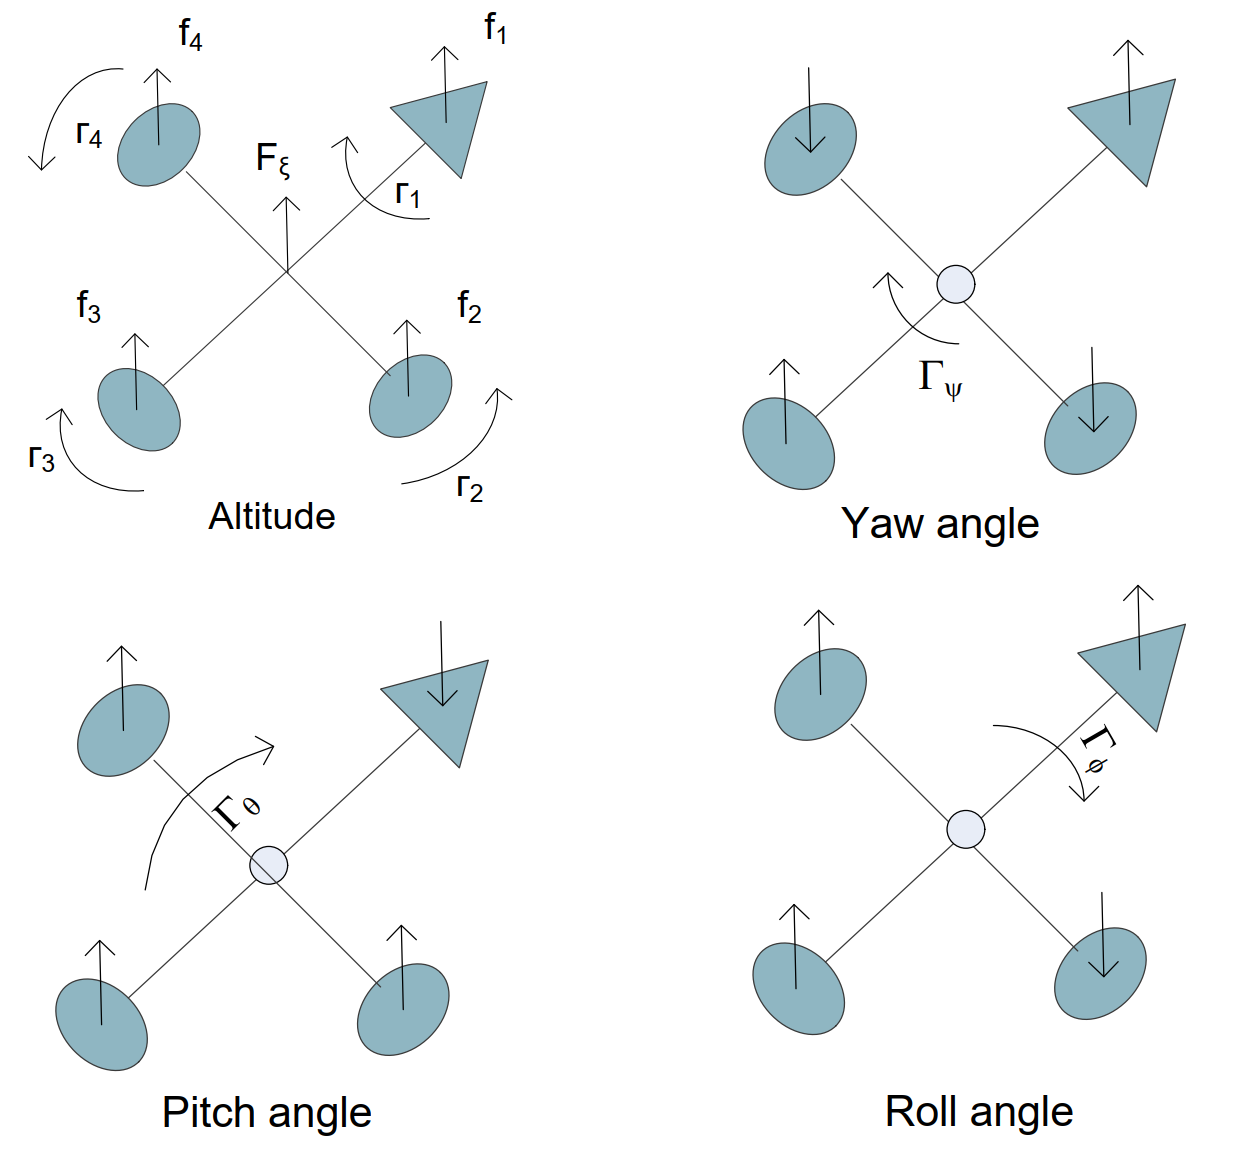
\includegraphics[width=0.6\textwidth]{Images/Modeling/Fantoni_a}
\caption{Model of the quadrotor represented with motor torques and Euler angles \cite{Fantoni2016}.}
\label{Fantoni_a}
\end{figure}

The equations of motion presented in the next subsection are based on the following assumptions:

\begin{itemize}
	\item The quadrotor has a rigid structure.
	\item The quadrotor has a symmetrical structure.
	\item The center of gravity (CoG) and the fixed frame at the center of the body are assumed to be coincident.
	\item The propellers of the quadrotor are assumed to be rigid.
	\item The thrust and drag forces are assumed to be proportional to the square of the spinning speed of each propeller.
\end{itemize}




















\subsection{Planar Quadrotor}\label{subsec:planar_quadrotor}

\begin{figure}[h]
	\centering
	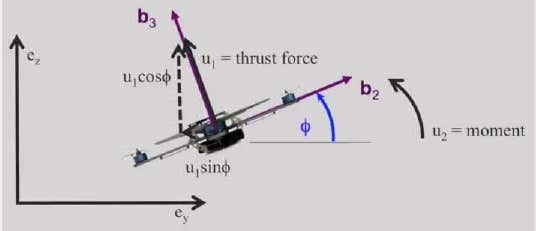
\includegraphics[width=0.7\textwidth]{Images/dynamics/planar_quadrotor.jpg}
	\caption{Representation of a planar drone. \cite{planar_quadrotor_figure}}
\end{figure}

The equations of motion of the planar quadrotor are:

\begin{equation}\label{dynamics_planar_quadrotor}
 \begin{cases} 
       \ddot{y} = - \frac{u_1}{m} \sin{\phi} \\
       \ddot{z} = - g + \frac{u_1}{m} \cos{\phi} \\
       \ddot{\phi} = \frac{u_2}{I_{xx}} \\
   \end{cases}
\end{equation}

With: 

\begin{itemize}
	\item $u_1$: Total thrust applied on the planar quadrotor.
	\item $u_2$: Torque applied by the planar quadrotor along the x-axis.
\end{itemize}

The dynamic model in equation (\ref{dynamics_planar_quadrotor}) assumes that the quadrotor is free to maneuver in the y-z plane. This means that the torque control input $u_2$ is only applied along the x-axis. 
Moreover, the equations of $\ddot{y}$ and $\ddot{z}$ represent the translational dynamics of the planar quadrotor, and they are controlled by $u_1$.
Furthermore, the equation of $\ddot{\phi}$ represents the rotational dynamics of the planar quadrotor, and it is controlled by $u_2$.
Finally, it should be noted that the total thrust $u_1$ is nothing else than the sum of the two thrust forces generated by the two rotors in the planar quadrotor.

\newpage

\subsection{3D Quadrotor}

In the case of the 3D quadrotor, the equations of motion can be expressed in different ways. They can either be expressed using the Euler angles $\phi, \theta, \psi$, which represent the roll, pitch and yaw angles respectively, or they can be expressed using quaternions. Both expressions will be presented below using the Newton-Euler formalism instead of the Lagrange-Euler formalism, since it is easier to implement when writing code.

\subsubsection{Equations of Motion with Euler Angles}\label{N_E_section}

\subsubsection*{Translational Model}

Based on Newton's second law:

\begin{equation}
	\sum \overrightarrow{F}=m\overrightarrow{a}
\end{equation}

with



\begin{itemize}
	\item $\overrightarrow{F}=\overrightarrow{F}_{\xi}=\begin{bmatrix}
F_x \\
F_y \\
F_z \\
\end{bmatrix}$ : vector of external forces.

\item $\overrightarrow{a} = \begin{bmatrix}
\ddot{x} \\
\ddot{y} \\
\ddot{z} \\
\end{bmatrix}$: accelerations vector.
\item $m$: mass of the quadrotor.
\end{itemize}

So, by applying Newton's second law on the quadrotor problem at hand:

\begin{equation*}
	m\begin{bmatrix}
	\ddot{x}\\
	\ddot{y}\\
	\ddot{z}\\
	\end{bmatrix} = \prescript{O}{}{\begin{bmatrix}
	0 \\
	0 \\
	-mg 
	\end{bmatrix}} + \prescript{U}{}{\begin{bmatrix}
	0 \\
	0 \\
	u 
	\end{bmatrix}} = \prescript{O}{}{\begin{bmatrix}
	0 \\
	0 \\
	-mg 
	\end{bmatrix}} + b \prescript{U}{}{\begin{bmatrix}
	0 \\
	0 \\
	\Omega_1^2 + \Omega_2^2 + \Omega_3^2 + \Omega_4^2
	\end{bmatrix}}
\end{equation*}

Where $u$ is the total thrust resulting from the 4 rotors. If $u$ is then expressed in the world frame, the equations of the translational model can be expressed as follows \cite{Fantoni2016}:

\begin{equation}\label{translation_model_N_E}
\begin{cases}
m \ddot{x} = (\sin \psi \sin \phi + \cos \psi \sin \theta \cos \phi)u \\
m \ddot{y} = (- \sin \phi \cos \psi + \sin \psi \sin \theta \cos \phi )u \\
m \ddot{z} = \cos \theta \cos \phi u -mg \\
\end{cases}
\end{equation}

\newpage

\subsubsection*{Rotational Model}

Based on the Newton-Euler equations, for a rotating frame \cite{Murray1994}: 

\begin{equation}\label{rotational_model_N_E_general_formula}
I \dot{\omega} + \omega \times I \omega = \tau
\end{equation}
with

\begin{itemize}
	\item $\bm{I} = \begin{bmatrix}
	I_{xx} && 0 && 0 \\
	0 && I_{yy} && 0 \\
	0 && 0 && I_{zz} \\
	\end{bmatrix}$
	\item $\bm{\eta}=\begin{bmatrix}
	p \\
	q \\
	r \\
	\end{bmatrix}$
	\item $\bm{\tau} = \begin{bmatrix}
	\tau_1 \\
	\tau_2 \\
	\tau_3 \\
	\end{bmatrix}$
\end{itemize}

Thus, equation (\ref{rotational_model_N_E_general_formula}) becomes:

\begin{equation}
\begin{bmatrix}
I_{xx}\dot{p}\\
I_{yy}\dot{q}\\
I_{zz}\dot{r}\\
\end{bmatrix}+ \begin{bmatrix}
qr(I_{zz}-I_{yy})\\
pr(I_{xx}-I_{zz})\\
pq(I_{yy}-I_{xx})
\end{bmatrix} = \begin{bmatrix}
\tau_1 \\
\tau_2 \\
\tau_3
\end{bmatrix}
\end{equation}


If equation \ref{total_torque_equation} is used, then input vector $\bm{\tau}$ can be substituted to acquire the final model of the rotation in the body frame:

\begin{equation}
\begin{cases}
\dot{p} = qr \frac{(I_{yy}-I_{zz})}{I_{xx}} + \frac{l}{I_{xx}}(f_4-f_2) - \frac{1}{I_{xx}}qJ_r (\Omega_1 - \Omega_2 + \Omega_3 - \Omega_4) \\
\dot{q} = pr \frac{(I_{zz}-I_{xx})}{I_{yy}} + \frac{l}{I_{yy}}(f_3-f_1) + \frac{1}{I_{yy}}pJ_r (\Omega_1 - \Omega_2 + \Omega_3 - \Omega_4) \\
\dot{r} = pq \frac{(I_{xx}-I_{yy})}{I_{zz}} + \frac{1}{I_{zz}} d (\Omega_1^2 -\Omega_2^2 + \Omega_3^2 - \Omega_4^2)
\end{cases}
\end{equation}

However, it can be inferred that the translational dynamics in  (\ref{translation_model_N_E}) and the rotational dynamics in (\ref{rotational_model_N_E_general_formula}) are highly nonlinear when they are expressed using Euler angles. And, this will result in high computational loads when they are included in a controller that solves an optimization problem at each time instant such as MPC. For this reason, it is simpler to express the dynamics of the quadrotor using quaternions. Quaternions are highly efficient for analyzing situations where rotations in $\mathbb{R}^3$ are considered. A quaternion is a 4-tuple, which is a more brief and simple representation of orientation when compared to a rotation matrix. Its geometric meaning is also more clear as the rotation axis and angle can be easily retrieved from it. In addition, quaternions allow the easy composition of rotations. This is due to the fact that composition of quaternions takes only sixteen multiplications and twelve additions \cite{jia_2013}. Thus, using quaternions will yield equations that are linear, which will result in ordinary differential equations (ODE's) that are easier to solve with MPC. In other words, when quaternions are used with a quadratic cost function, such as a linear least-squared cost function, the optimization problem becomes convex, which has a global minimum, as shown in figure \ref{convex_function}.

\newpage

\subsubsection{Equations of Motion with Quaternions}\label{equations_of_motion_quaternion_form}

The equations of motion of a quadrotor expressed with quaternions are \cite{Erskine2021}:

				\begin{align}\label{translation_model_quaternion}
					\text{Translational model: }\left\{
					\begin{array}{ll}				
					\dot{\bm{p}_i} &= \bm{v}_i \\
					\dot{\bm{v}_i} &= 
					\frac{T}{m} 
					\begin{bmatrix}
						2 (q_w q_y + q_x q_z) \\
						2 (q_y q_z - q_w q_x) \\
						1 - 2(q_x^2 + q_y^2 ) \\
					\end{bmatrix} + \bm{g} \\	
					\end{array}
					\right.
				\end{align}
				\begin{align}\label{rotational_model_quaternion}
			\text{Rotational model: }\left\{
			\begin{array}{ll}		
					\dot{\bm{q}_i} & = \frac{1}{2}
					\begin{bmatrix}
						0 \\
						\bm{\omega}_i \\
					\end{bmatrix} \otimes \bm{q}_i \\
					\dot{\bm{\omega}_i} &= \bm{I}_i^{-1} \bm{\tau}_i - \bm{I}_i^{-1} (\bm{\omega}_i \times \bm{I}_i \bm{\omega}_i)
			\end{array}
			\right.
				\end{align}
			
The 2 equations in (\ref{translation_model_quaternion}) represent the first order kinematics and the second order dynamics of the translational model of the system respectively. Similarly, the 2 equations in (\ref{rotational_model_quaternion}) represent the first order kinematics and the second order dynamics in the rotational model of the system respectively. 
Moreover, this model will be used for the remainder of this report for performing simulations in both the acados interface, and in ROS2/Gazebo. 

It is clear that the elements of the body torques vector $\bm{\tau}$ are not being computed using this model. This is because there exists a direct linear mapping between the angular acceleration $\bm{\dot{\bm{\omega}}}$ and the body torques $\bm{\tau}$. In other words, $\bm{\tau}$ can be computed from $\bm{\dot{\bm{\omega}}}$ .

However, since a non-centralized MPC structure will be designed to reduce the computation time, then the MPC controller will not account for all the equations of motion in (\ref{translation_model_quaternion}) and (\ref{rotational_model_quaternion}). In fact, they will be distributed as follows: 

				\begin{equation*}
					\text{Treated by the MPC: }\left\{
					\begin{array}{lll}				
					\dot{\bm{p}_i} &= \bm{v}_i \\
					\dot{\bm{v}_i} &= 
					\frac{T}{m} 
					\begin{bmatrix}
						2 (q_w q_y + q_x q_z) \\
						2 (q_y q_z - q_w q_x) \\
						1 - 2(q_x^2 + q_y^2 ) \\
					\end{bmatrix} + \bm{g} \\			
					\dot{\bm{q}_i} & = \frac{1}{2}
					\begin{bmatrix}
						0 \\
						\bm{\omega}_i \\
					\end{bmatrix} \otimes \bm{q}_i \\
					\end{array}
					\right.
				\end{equation*}
				
				\begin{equation*}
					\text{Treated by the Low-Level Controller: }\left\{
					\begin{array}{l}	
					\dot{\bm{\omega}_i} = \bm{I}_i^{-1} \bm{\tau}_i - \bm{I}_i^{-1} (\bm{\omega}_i \times \bm{I}_i \bm{\omega}_i)
					\end{array}
					\right.
				\end{equation*}

Moreover, the control inputs that will be outputted by the MPC controller are: 

\begin{itemize}
	\item $T$: The total thrust force.
	\item $\omega_x, \omega_y, \omega_z$: The angular rates. 
\end{itemize} 

\newpage

\begin{figure}[h]
	\centering
	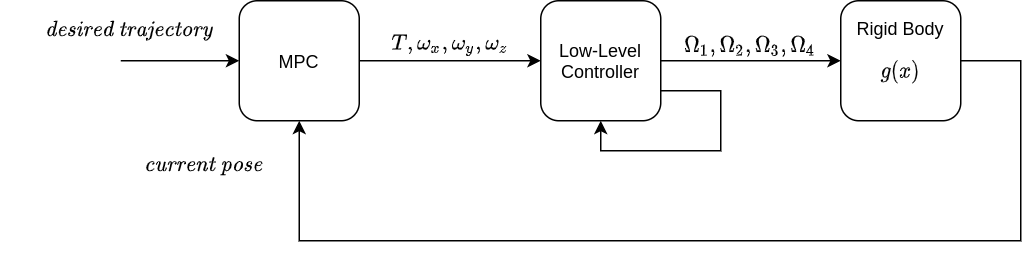
\includegraphics[width=\textwidth]{Images/diagrams/new_sim_diagram.png}
	\caption{Diagram of the resulting non-centralized MPC closed-loop control structure.}
	\label{non_centralized_mpc_for_SIL}
\end{figure}

As shown in figure \ref{non_centralized_mpc_for_SIL}, the MPC controller will solve an optimization problem at each iteration, and will output the total thrust $T$, and the angular rates $\omega_x, \omega_y$ and $\omega_z$, which will be fed to the low-level controller. Then, the low-level controller will map the angular rates to the body torques. Afterwards, the total thrust $T$ and the body torques $\bm{\tau}$ will then be converted to motor speeds, which will be outputted to the quadrotor in order to follow a desired trajectory.

\section{Extended Kalman Filter for the Planar Quadrotor}
In order to perform simple simulations with acados in the planar case under the presence of disturbance, it is useful to design an Extended Kalman Filter (EKF) for the planar quadrotor in order to reduce the effects of the noise on the system and increase the tracking accuracy of a desired trajectory. The Extended Kalman Filter was chosen instead of the Kalman Filter (KF) because the Kalman Filter works well for linear systems. However, the quadrotor dynamics are highly  nonlinear as seen in (\ref{subsec:planar_quadrotor}), which the Extended Kalman Filter can handle well. The EKF works by linearizing the nonlinear equations of motion at each time step. This is done by using the current values of the state vector of the planar quadrotor, in addition to the Jacobian matrices of the state vector. However, it should be noted that the EKF will not provide proper measurements if the initial condition of the state vector is not properly defined. The equations used are from the following reference \cite{AUVE2020}.

\subsection{Evolution Model}

The state vector used for the planar quadrotor is: 
\begin{equation}\label{planar_drone_states}
	X = \begin{bmatrix}
		y & z & \phi & v_y & v_z & \dot{\phi} \\ 
	\end{bmatrix}^{\intercal}
\end{equation}

So, the evolution model can be expressed as follows: 

\begin{equation}\label{evolution_model}
        \begin{bmatrix}
            y_{k+1} \\ z_{k+1} \\ \phi_{k+1} \\ v_{y_{k+1}} \\ v_{z_{k+1}} \\ \dot{\phi}_{k+1} 
        \end{bmatrix} = 
        \begin{bmatrix}
            y_{k} \\ z_{k} \\ \phi_{k} \\ v_{y_{k}} \\ v_{z_{k}} \\ \dot{\phi}_{k} 
        \end{bmatrix}
        + \Delta t \begin{bmatrix} 
            v_{y_{k}} \\ v_{z_{k}} \\ \dot{\phi}_{k} \\ -\frac{u_{1_k}}{m} \sin \phi_k \\ -g + \frac{u_{1_k}}{m} \cos \phi_k \\ \frac{u_2}{I_{xx}}
        \end{bmatrix}
    \end{equation}
With $\Delta t$ being the sample time.

\newpage    
    
	\subsection{Measurement Model}
	
	Generally, quadrotors make use of an embedded Inertial Measurement Unit (IMU) sensor, which typically measures angular rates and body-frame accelerations. In addition, an embedded air pressure sensor can also be used to measure the altitude of the quadrotor. However, since simple simulations will be conducted in acados, it is assumed the all the states can be measured. This will result in the following measurement model:
	
	\begin{equation}\label{measurement_model}
        Y = CX = I_{6 \times 6} X = [y, z, \phi, v_y, v_z, \dot{\phi}]^{\intercal}
    \end{equation}

So, in this very simplified case, the measurement vector is identical to the state vector.
Moreover, for the case of the 3D drone, the quadrotor that will be used already has an EKF implemented that is able to take inputs from different sensors and fuse them in order to output filtered measurements.
A figure showing a representation of the EKF implemented on the real quadrotor with all the available inputs and outputs is shown below:

\begin{figure}[h]
	\centering
	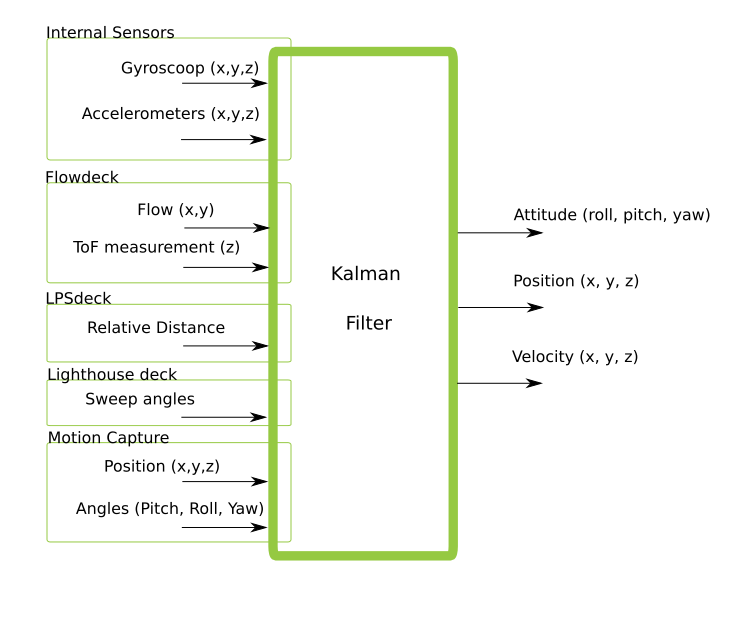
\includegraphics[width=.5\textwidth]{Images/ekf/extended_kalman_filter.png}
	\caption{Diagram of the EKF embedded in the crazyflie2.1 \cite{EKF_bitcraze}.}
	\label{ekf_diagram_crazyflie}
\end{figure}

	\subsection{Prediction Phase}
	In the prediction phase, no measurement is taken. The state is predicted using the evolution model and Jacobian matrices of the state vector.
	
Using the state vector and the control inputs of the previous time instant, the current state vector can predicted using the evolution in model in \ref{evolution_model}. So,
    \begin{equation}
        X_k = evolution(X_{k-1}, U_{k-1},\Delta t)
    \end{equation}

And, in order to show how accurate the prediction is, a covariance matrix for the prediction is computed as follows:

    \begin{equation}
        P_k = A_{k-1} P_{k-1} A_{k-1}^{\intercal} + B_{k-1} Q_{\beta} B_{k-1}^{\intercal} + Q_{\alpha}
    \end{equation}

Where: 

\begin{itemize}
	\item $P_{k-1}$: the covariance matrix of the previous time instant.
	\item $A_{k-1}$: the Jacobian of the state vector with respect to each state at the previous time instant.
	\item $B_{k-1}$: the Jacobian of the state vector with respect to the control inputs at the previous time instant.
	\item $Q_{\alpha}$: the covariance matrix of the state noise.
	\item $Q_{\beta}$: the covariance matrix of the input noise.
\end{itemize}	

And, the expressions of $A_{k-1}$ and $B_{k-1}$ are:

\begin{equation}
        A_{k-1} = \begin{bmatrix}
                1 & 0 & 0 & \Delta t  & 0 & 0 \\
                0 & 1 & 0 & 0  & \Delta t & 0 \\
                0 & 0 & 1 & 0 & 0 & \Delta t \\
                0 & 0 & -\frac{u_{1_{k-1}}}{m} \cos \phi_{k-1} \Delta t & 1 & 0 & 0 \\
                0 & 0 & -\frac{u_{1_{k-1}}}{m} \sin \phi_{k-1} \Delta t & 0 & 1 & 0 \\
                0 & 0 & 0 & 0 & 0 & 1 \\
            \end{bmatrix}
    \end{equation}
    \begin{equation}
        B_{k-1} = \begin{bmatrix}
            0 & 0 \\
            0 & 0 \\
            0 & 0 \\
            - \frac{\sin \phi_{k-1}}{m} \Delta t & 0 \\
            - \frac{\cos \phi_{k-1}}{m} \Delta t & 0 \\
            0 & \frac{\Delta t}{I_{xx}} \\
        \end{bmatrix}
    \end{equation}
    
In addition, the expression of $Q_{\alpha}$ was found using trial and error based on the amount of noise added on the state and the inputs:

\begin{equation}
        Q_{\alpha} = \begin{bmatrix}
                10^{-7} & 0 & 0 & 0  & 0 & 0 \\
                0 & 10^{-4} & 0 & 0  & 0 & 0 \\
                0 & 0 & 10^{-5} & 0 & 0 & 0 \\
                0 & 0 & 0 & 10^{-7} & 0 & 0 \\
                0 & 0 & 0 & 0 & 10^{-4} & 0 \\
                0 & 0 & 0 & 0 & 0 & 10^{-5} \\
            \end{bmatrix}
\end{equation}
With each value representing the variance of the state noise on each element of the state vector. It is important not to have $Q_{\alpha}=0_{6 \times 6}$ because in the case of the planar quadrotor, the previous states have a great influence on the evolution model as can be seen in (\ref{evolution_model}).

As for the covariance matrix of the input noise $Q_{\beta}$:

\begin{equation}
	Q_{\beta} = \begin{bmatrix}
	(10^{-3})^2 & 0 \\
	0 & (10^{-4})^2 \\
	\end{bmatrix}
\end{equation}

Where the first diagonal term represents the variance of the noise on the thrust input $u_1$. This variance represents an input noise between $-0.001N$ and $0.001N$. As for the second diagonal term, it represent the variance of the noise on the torque input $u_2$. This variance represents  an input noise between $-0.0001N.m$ and $0.0001N.m$. The variance values were chosen to be small because the quadrotor used will have a maximum thrust of $0.45N$, as will be shown in future sections, which is already very small. 

\newpage

In addition, the covariance matrix of the initial state is chosen to be:

\begin{equation}
P_0 = \begin{bmatrix}
                10^{-2} & 0 & 0 & 0  & 0 & 0 \\
                0 & 10^{-2} & 0 & 0  & 0 & 0 \\
                0 & 0 & 10^{-2} & 0 & 0 & 0 \\
                0 & 0 & 0 & 10^{-2} & 0 & 0 \\
                0 & 0 & 0 & 0 & 10^{-2} & 0 \\
                0 & 0 & 0 & 0 & 0 & 10^{-2} \\
            \end{bmatrix}
\end{equation}

$P_0$ represents the accuracy of the initial condition of the state vector.

	\subsection{Correction Phase}
	The correction phase is where the measurement from the sensors are taken and fused with the outputs of the predicted state to provide a proper estimation of the state.
	
First, the measurement prediction is computed: 

	\begin{equation}
        \hat{Y}_k = C X_k 
    \end{equation}
    
    Where $C \equiv	I_{6 \times 6}$, similarly to (\ref{measurement_model}).

Then, the Kalman gain is computed as follows:

\begin{equation}
        K = P_k C^{\intercal} (C P_k C^{\intercal} + Q_{\gamma})^{-1}
    \end{equation}

Where, $Q_{\gamma}$ is the covariance matrix of the measurement noise. The square root of each diagonal term in $Q_{\gamma}$ was used as the magnitude for added white Gaussian noise of the corresponding state. So, $Q_{\gamma}$ was chosen to be:

 \begin{equation}
        Q_{\gamma} = \begin{bmatrix}
                (10^{-2})^2 & 0 & 0 & 0  & 0 & 0 \\
                0 & (10^{-2})^2 & 0 & 0  & 0 & 0 \\
                0 & 0 & (\frac{\pi}{180})^2 & 0 & 0 & 0 \\
                0 & 0 & 0 & (10^{-3})^2 & 0 & 0 \\
                0 & 0 & 0 & 0 & (10^{-3})^2 & 0 \\
                0 & 0 & 0 & 0 & 0 & (\frac{\pi}{180})^2 \\
            \end{bmatrix}
\end{equation}

The diagonal terms in $Q_{\gamma}$ mean the following:

\begin{itemize}
	\item The added noise on $y$ is between $-1cm$ and $1cm$.
	\item The added noise on $z$ is between $-1cm$ and $1cm$.
	\item The added noise on the roll angle $\phi$ is between $-1^{\circ}$ and $1^{\circ}$
	\item The added noise on $v_y$ is between $-0.01m/s$ and $0.01m/s$.
	\item The added noise on $v_z$ is between $-0.01m/s$ and $0.01m/s$.
	\item The added noise on $\dot{\phi}$ is between $-1^{\circ}/s$ and $1^{\circ}/s$.
\end{itemize}
    
    \newpage
    
    In addition, the state vector is updated as follows:
    
    \begin{equation}
        X_k = X_k + K (Y_k-\hat{Y}_k)
    \end{equation}
    
    Finally, the covariance matrix of the state vector is updated. There exist many formulas to update the covariance matrix of the state after the state vector has been corrected. However, the Joseph form was used since it is better conditioned when compared to the other available formulas. So, the covariance matrix of the state vector is updated using the following: 
    
    \begin{equation}
        P_k = ( I - K C) P_k ( I - K C)^{\intercal} + K Q_{\gamma} K^{\intercal}
    \end{equation}

\section{Design of the MPC controller}

\subsection{Parameters of the Crazyflie 2.1}\label{subsec:parameters_of_the_crazyflie}

The parameters of crazyflie were identified in \cite{Forster2015}. However, to increase the accuracy of the simulations that will be performed, the drone was weighed using a small scale to determine its actual mass.

\begin{figure}[h]
	\centering
	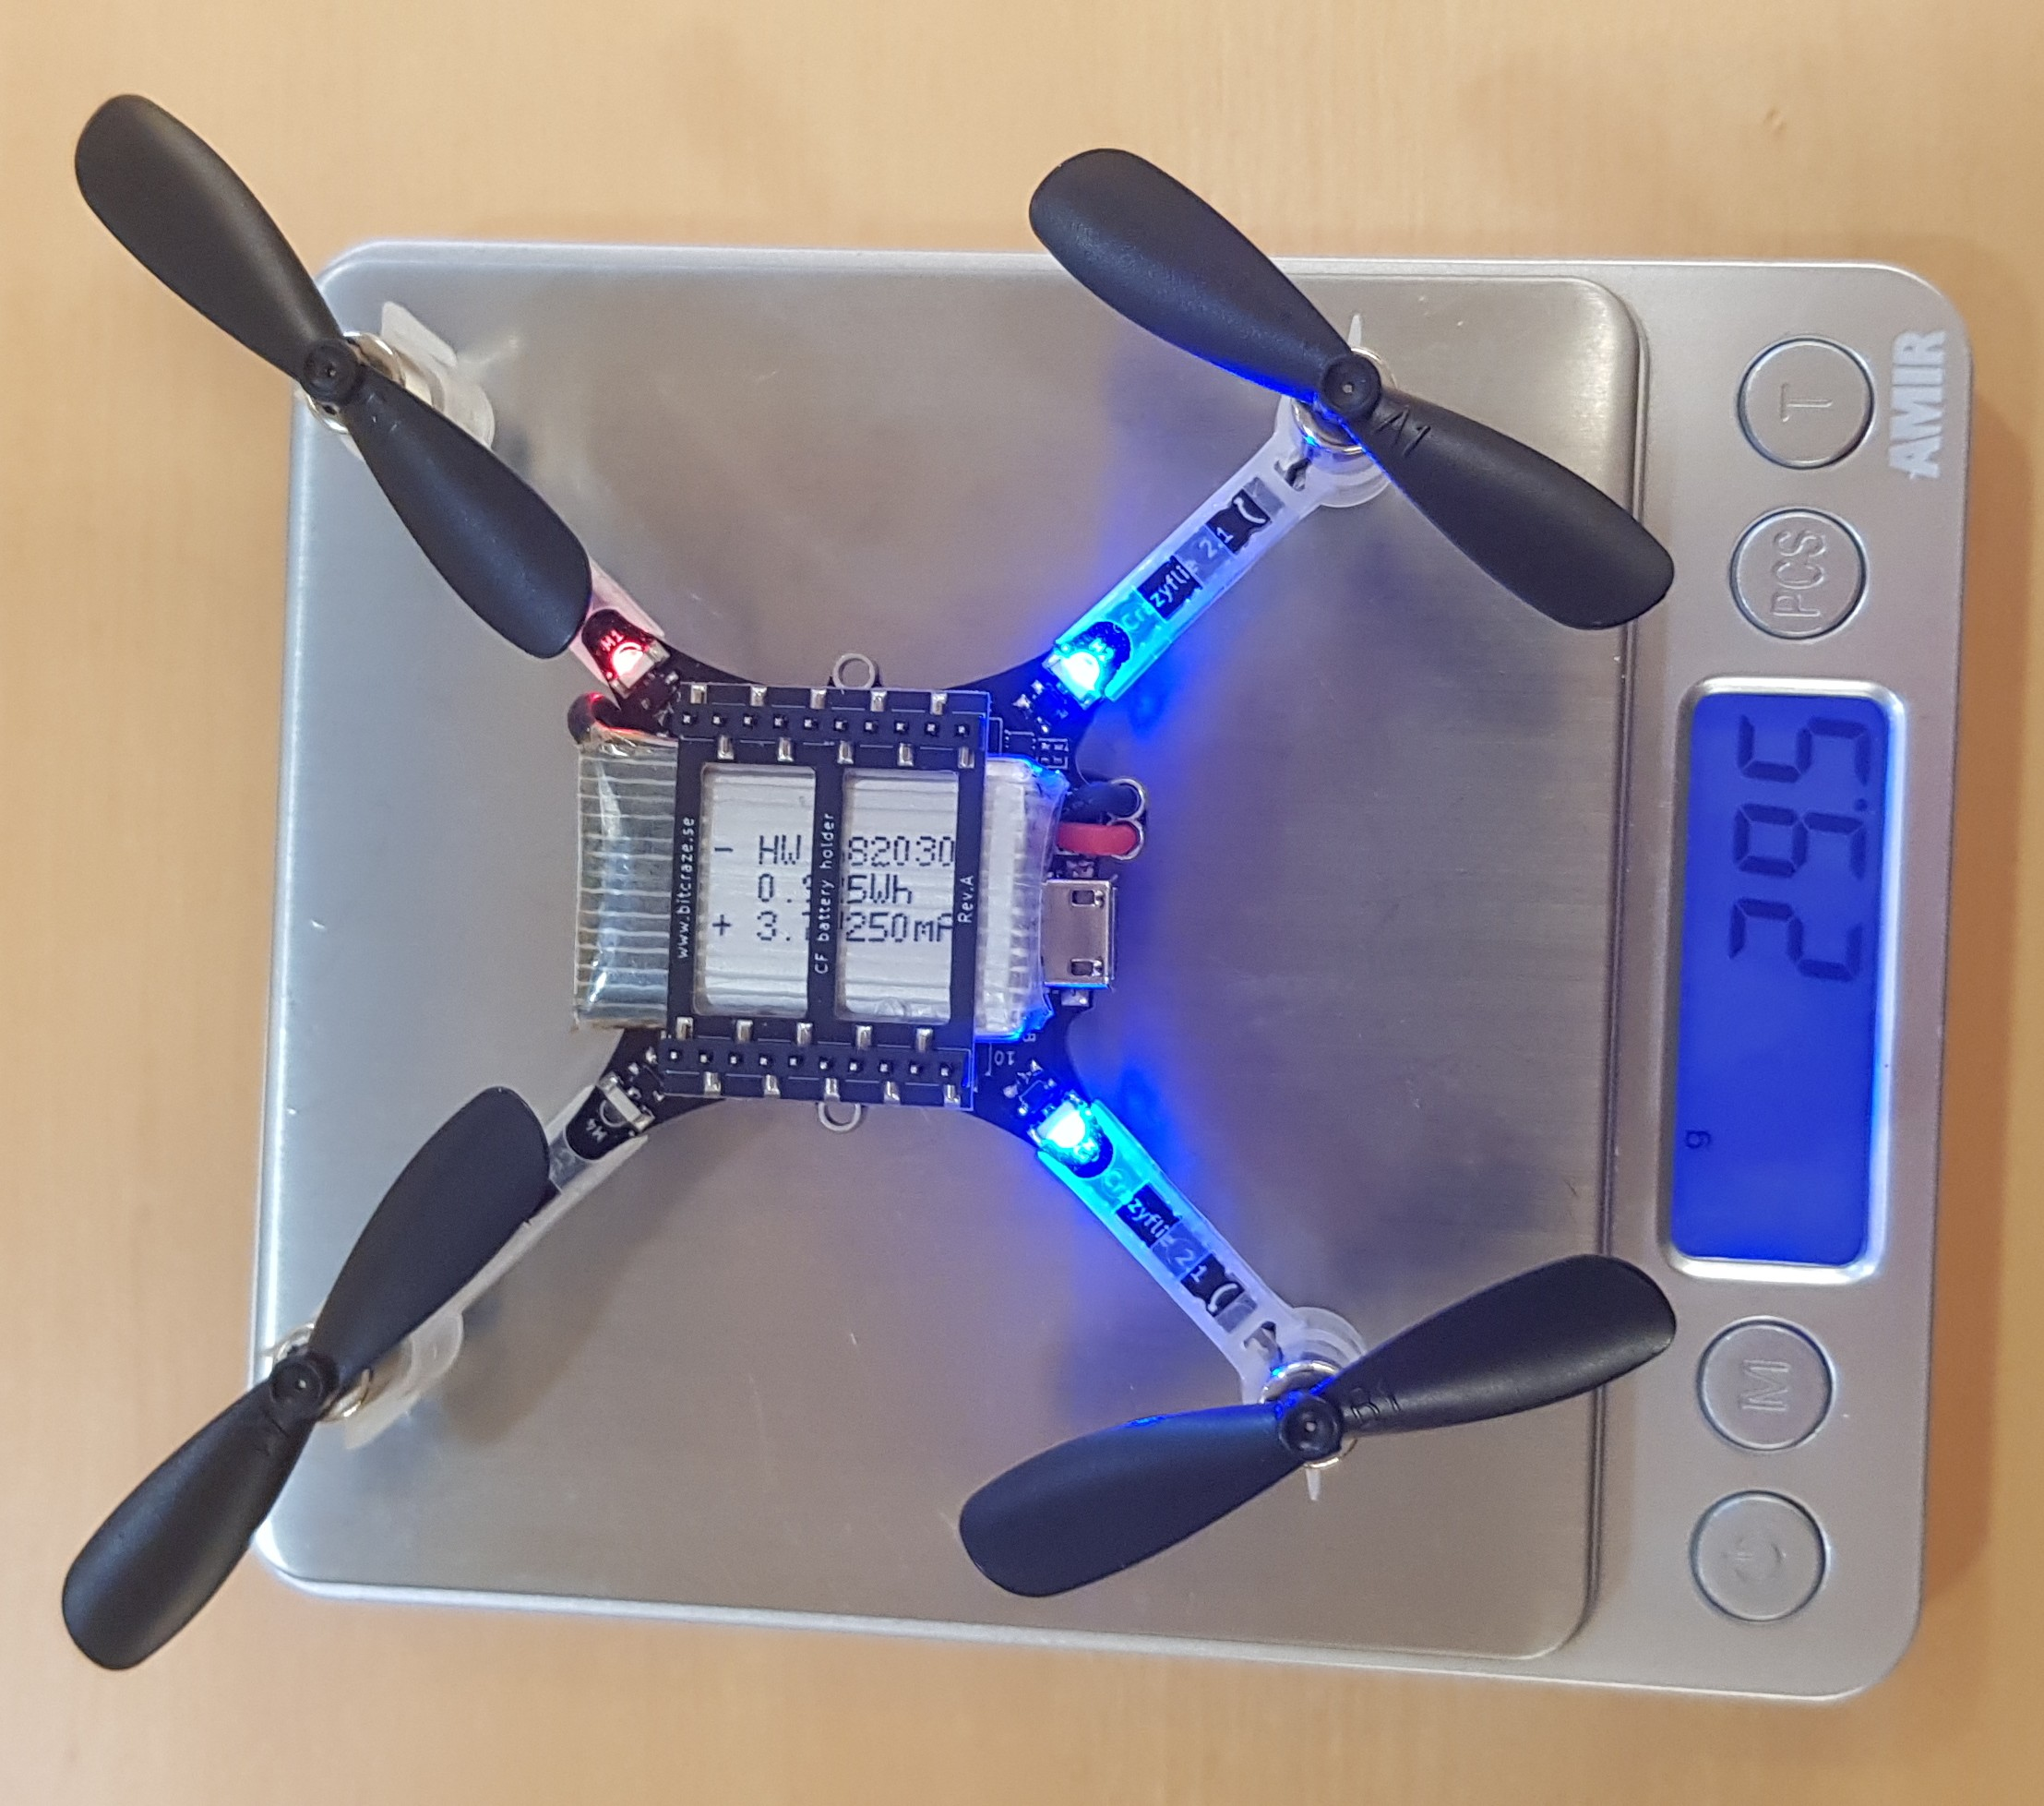
\includegraphics[width=0.6\textwidth, angle =-90]{Images/crazyflie/weight.jpg}
	\caption{Mass of the crazyflie 2.1 equiped with the battery and properllers.}
	\label{fig:crazyflie_weight}
\end{figure}

As can be seen in figure \ref{fig:crazyflie_weight}, the mass of the crazyflie is $29.5g$. However, it should be noted that the crazyflie is marketed to have a mass of $27g$ as shown in the crazyflie 2.1 datasheet \cite{crazyflie_datasheet}.

Then, in order to find the maximum thrust, several experiments were conducted with different added masses to the quadrotor. And, the maximum thrust was found when the quadrotor was barely able to support its weight and hover.

\newpage

\begin{figure}[h]
	\centering
	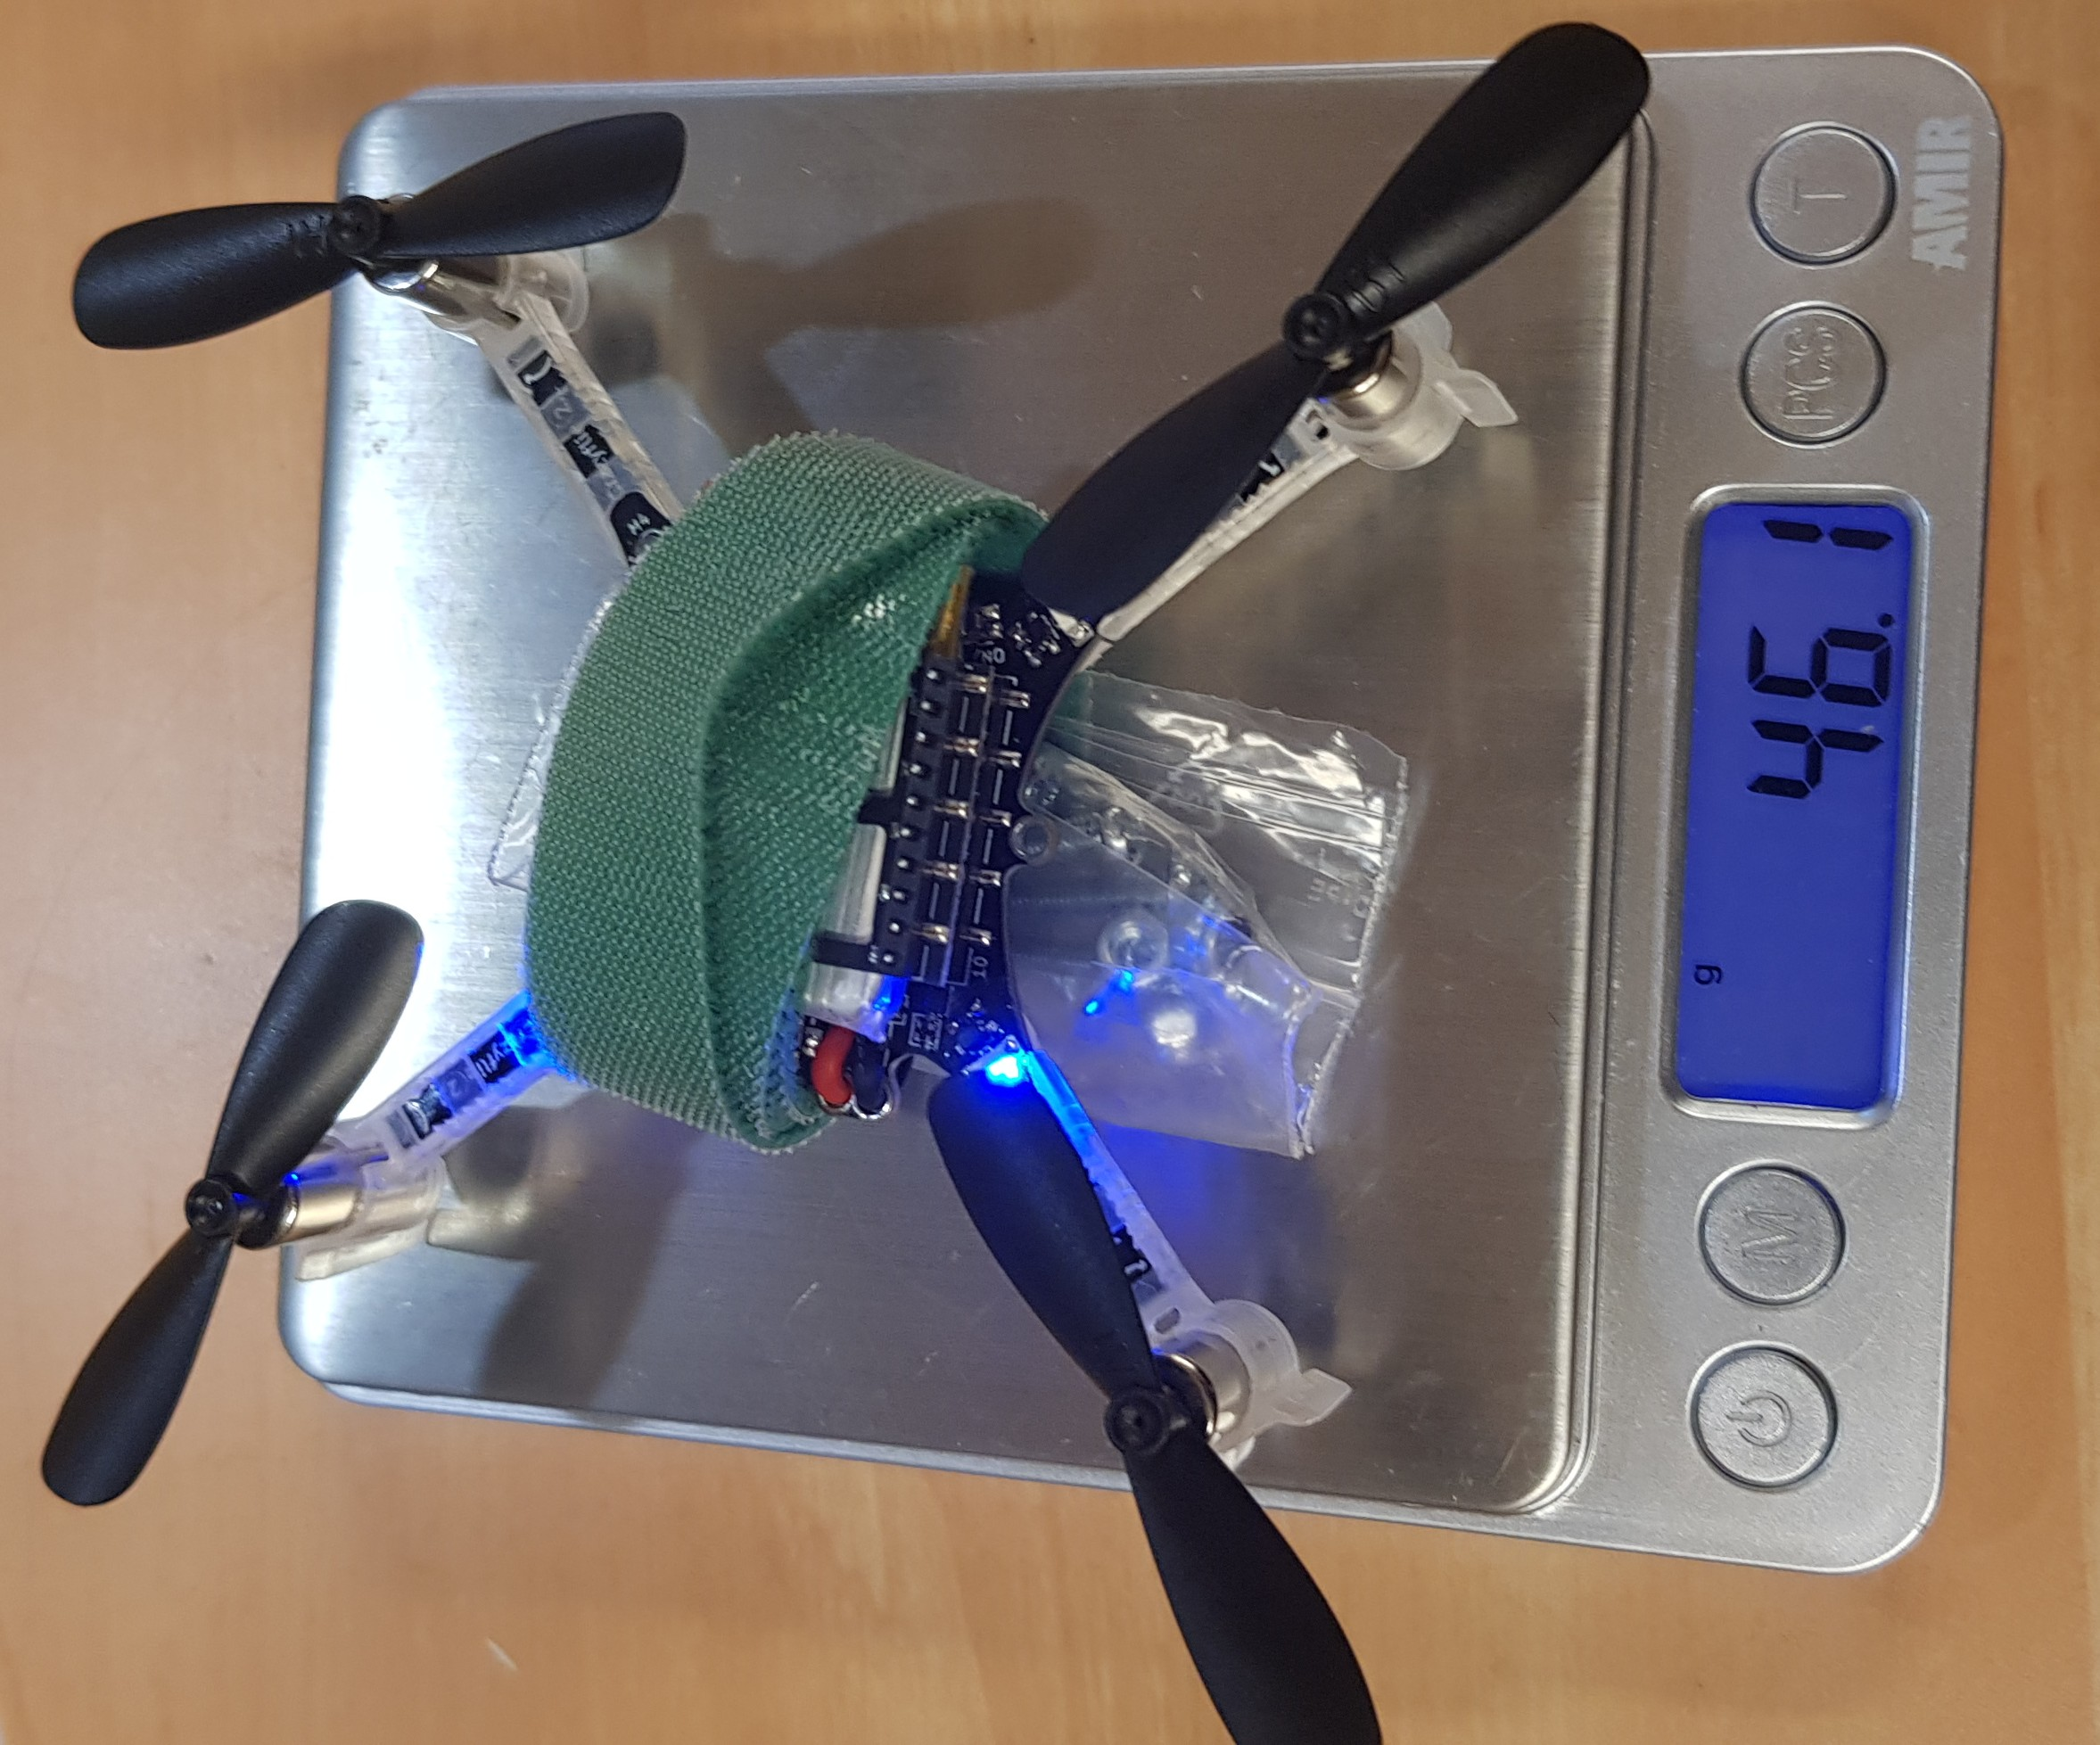
\includegraphics[width=0.6\textwidth, angle =-90]{Images/crazyflie/max_thrust.jpg}
	\caption{Mass of the crazyflie 2.1 with the maximum added mass that it can support.}
	\label{fig:max_thrust}
\end{figure}

As can be seen in figure \ref{fig:max_thrust}, the maximum thrust was found when the crazyflie had a total mass of $46g$. So, the maximum thrust of the drone is:

\begin{equation}
	T_{max}^{actual} = 46 \times 10^{-3} kg \times 9.81 \frac{m}{s^2} = 0.45126 N
\end{equation}

So, the parameters of the quadrotor that will be used in all the simulations are:

\begin{itemize}
	\item $m = 0.0295 kg$
	\item $I_{xx}$ = $1.657171 \times 10^{-5} N.m$
	\item $I_{yy}$ = $1.657171 \times 10^{-5} N.m$
	\item $I_{zz}$ = $2.9261652 \times 10^{-5} N.m$
	\item $l = 0.046m$
	
\end{itemize}

It should be noted that in the case of the planar quadrotor, the mass and the total thrust will be divided by 2 since only 2 rotors will be present instead of 4 in the planar case.

In addition, the maximum thrust is never used. Because, when the maximum thrust is applied by the quadrotor, the quadrotor will not be able to do move freely in space. In other words, the quadrotor will only be able to move vertically and hover at a desired position. As a result, a general rule of thumb is to set the maximum thrust to be 90\% of the actual maximum. This way, the remaining 10\% of the thrust can be used to control the torque in order to perform maneuvers and move in the 3D space. In addition, the planar drone will also be restricted to keeping only a 10\% margin for steering torque. This is done because the maximum torque $\tau_{max}$ is the maximum torque that can be given around any one axis. However, the torque must be limited greatly in order to stabilize and have more control of the quadrotor. These constraints are set in the MPC controller when it is being designed.

\newpage

\subsection{Planar Quadrotor MPC}

The MPC optimization problem is formulated as follows:

	\begin{equation}\label{mpc_optimization_problem_planar_quadrotor}
\begin{aligned}
            \min_{x,u} \quad & \frac{1}{2}\|\bm{V}_x \bm{x} + \bm{V}_u \bm{u} + \bm{V}_z \bm{z} - \bm{y}_{ref}\|^2_{\bm{W}} + \frac{1}{2}\|\bm{V}_x^e \bm{x} - \bm{y}_{ref}^e \|^2_{\bm{W}_e} \\
            \textrm{s.t.} \quad & f(\bm{x},\bm{u}):\text{dynamics} \\
            & 0 \leq T \leq T_{max} \\
            & - \tau_{max} \leq \tau \leq \tau_{max}
        \end{aligned}
\end{equation}
with: 
\begin{multicols}{3}
\begin{itemize}
	\item $\bm{V}_x \in \mathbb{R}^{n_y \times n_x}$
	\item $\bm{V}_u \in \mathbb{R}^{n_y \times n_u}$ 
	\item $\bm{V}_z \in \mathbb{R}^{n_y \times n_z}$
	\item $\bm{V}_x^e \in \mathbb{R}^{n_{ye}\times n_x}$
\end{itemize}
\columnbreak
\begin{itemize}
	\item $\bm{y}_{ref} \in \mathbb{R}^{n_y}$
	\item $\bm{y}_{ref_e} \in \mathbb{R}^{n_{y_e}}$
	\item $\bm{W} \in \mathbb{R}^{n_y \times n_y}$
	\item $\bm{W}_e \in \mathbb{R}^{n_{y_e} \times n_{y_e}}$
\end{itemize}
\columnbreak
\begin{itemize}
	\item $\bm{Q},\bm{Q}_e \in \mathbb{R}^{n_x \times n_x}$
	\item $\bm{R} \in \mathbb{R}^{n_u \times n_u}$
	\item $\bm{W} = diag(\bm{Q},\bm{R}) $
	\item $\bm{W}_e = \bm{Q}_e $
\end{itemize}
\end{multicols}

And, by taking the state vector as shown in (\ref{planar_drone_states}) and by using the equations of motion of the planar quadrotor as shown in (\ref{dynamics_planar_quadrotor}), it is evident that the states evolve according to:

			\begin{align}
                \dot{y} &= v_y \\
                \dot{z} &= v_z \\
                \dot{\phi} &= \dot{\phi} \equiv \dot{roll} \\
                \dot{v}_y &= - \frac{u_1}{m} \sin(\phi) \\
                \dot{v}_z &= - g + \frac{u_1}{m} \cos(\phi) \\
                \ddot{\phi} &= \frac{u_2}{I_{xx}}
            \end{align}   

As shown in \ref{subsec:planar_quadrotor}, the control inputs vector in this case is :
	\begin{equation}
	\bm{u} = \begin{bmatrix}
		u_1 & u_2 \\
	\end{bmatrix}^{\intercal}
	\end{equation}

Then, the initial condition of the states of the quadrotor is set: 

\begin{equation}
	\bm{x}_0 = \begin{bmatrix}
	x_0 & y_0 & \phi_0 & v_{y_0} & v_{z_0} & \dot{\phi}_0 \\
	\end{bmatrix}^{\intercal}
\end{equation} 

And, the desired trajectory will be fed to the MPC controller as a reference by using the future $N$ waypoints of the trajectory, which contain the desired states at each time instant:

\begin{equation}
	\bm{x}_d = \begin{bmatrix}
		x_d & y_d & \phi_d & v_{y_d} & v_{z_d} & \dot{\phi}_d \\
\end{bmatrix}^{\intercal}	 
\end{equation}

Furthermore, the desired control inputs $\bm{u}_d$ can also be fed to the MPC controller:


\begin{equation}
	\bm{u}_d = \begin{bmatrix}
		u_{1_d} & u_{2_d} \\
	\end{bmatrix}^{\intercal}
\end{equation}

 The reference vector $\bm{y}_{ref}$ in the running cost can be constructed using the desired waypoints and the desired control inputs for the next $(N-1)$ time steps:

\begin{equation}
	\bm{y}_{ref} = \begin{bmatrix}
		\bm{x}_d^{\intercal} & \bm{u}_d^{\intercal} \\
	\end{bmatrix}^{\intercal}
\end{equation}

The reference vector $\bm{y}_{ref}^e$ in the terminal cost contains the desired waypoint at time step $N$:
\begin{equation}
	\bm{y}_{ref}^e = \bm{x}_d
\end{equation}

\newpage

Moreover, the MPC parameters are chosen to be:
\begin{itemize}
	\item $N = 100$ : number of discretization steps in the prediction horizon.
	\item $T_f = 1s$ : prediction horizon.
\end{itemize}

It should be noted that the number of discretization steps that was used is rather large, and will surely be reduced during the experimentation phase. However, it was still used in the simple acados simulations since the total computation time of the MPC while tracking a $22s$ trajectory as around $8.5s$ on an Inter Core i5-6300u 2.4GHz with 4 cores, which can be considered as a mid-range processor. An example of a MPC computation time for a planar quadrotor which is tracking a circular trajectory is shown in figure \ref{fig:computation_time_planar_quadrotor} below.

\begin{figure}[h]
	\centering
	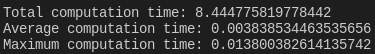
\includegraphics[width=0.7\textwidth]{Images/acados_simulations/circular_trajectory/planar_drone/computation_time.png}
	\caption{Computation of the MPC for a planar quadrotor tracking a 22s trajectory.}
	\label{fig:computation_time_planar_quadrotor}
\end{figure}

Finally, the maximum thrust and torque are computed as explained in \ref{subsec:parameters_of_the_crazyflie}: 

	\begin{equation}
		T_{max} = 0.9 (\frac{T_{max}^{actual}}{2})=0.203067N
	\end{equation}
	
	\begin{equation}
		\tau_{max} = 0.1(\frac{1}{2}T_{max}l)=0.0004670541N.m
	\end{equation}

And, as for the components of the linear least-squared cost function:

\begin{multicols}{2}
        \begin{itemize}
                \item $\bm{V}_x = \begin{bmatrix}
                1 & 0 & 0 & 0 & 0 & 0 \\
                0 & 1 & 0 & 0 & 0 & 0 \\
                0 & 0 & 1 & 0 & 0 & 0 \\
                0 & 0 & 0 & 1 & 0 & 0 \\
                0 & 0 & 0 & 0 & 1 & 0 \\
                0 & 0 & 0 & 0 & 0 & 1 \\
                0 & 0 & 0 & 0 & 0 & 0 \\
                0 & 0 & 0 & 0 & 0 & 0 \\
                \end{bmatrix}$
                
                \item $\bm{V}_{x_e} = \begin{bmatrix}
                1 & 0 & 0 & 0 & 0 & 0 \\
                0 & 1 & 0 & 0 & 0 & 0 \\
                0 & 0 & 1 & 0 & 0 & 0 \\
                0 & 0 & 0 & 1 & 0 & 0 \\
                0 & 0 & 0 & 0 & 1 & 0 \\
                0 & 0 & 0 & 0 & 0 & 1 \\
                \end{bmatrix}$
                
                \item $\bm{V}_u = \begin{bmatrix}
                0 & 0 \\
                0 & 0 \\
                0 & 0 \\
                0 & 0 \\
                0 & 0 \\
                0 & 0 \\
                1 & 0 \\
                0 & 1 \\
                \end{bmatrix}$
                
            \end{itemize}
			\columnbreak
            \begin{itemize}
            	\item $\bm{Q} = \begin{bmatrix}
                 30 & 0  & 0 & 0 & 0 & 0 \\
                 0 & 30  & 0 & 0 & 0 & 0 \\
                 0 & 0  & 0 & 0 & 0 & 0 \\
                 0 & 0  & 0 & 5 & 0 & 0 \\
                 0 & 0  & 0 & 0 & 5 & 0 \\
                 0 & 0  & 0 & 0 & 0 & 0 \\
                \end{bmatrix}$
                
                \item $\bm{Q}_e = \begin{bmatrix}
                 30 & 0  & 0 & 0 & 0 & 0 \\
                 0 & 30  & 0 & 0 & 0 & 0 \\
                 0 & 0  & 0 & 0 & 0 & 0 \\
                 0 & 0  & 0 & 5 & 0 & 0 \\
                 0 & 0  & 0 & 0 & 5 & 0 \\
                 0 & 0  & 0 & 0 & 0 & 0 \\
                \end{bmatrix}$
                
                \item $\bm{R} = \begin{bmatrix}
                1 & 0 \\
                0 & 1 \\
                \end{bmatrix}$
                
            \end{itemize}
\end{multicols}

The matrices $\bm{V}_x$ and  $\bm{V}_u$ are used to refer to each element of the state in the state vector $\bm{x}$ and to each element of the inputs in the input vector $\bm{u}$ in the running cost, respectively. And, it should be noted that there are no algebraic variables $\bm{z}$ in the problem at hand. However, it is included in the cost function of equation (\ref{mpc_optimization_problem_planar_quadrotor}) for completeness. Furthermore, the matrix $\bm{V}_{x_e}$ is used to refer to each element of the state vector $\bm{x}$ in the terminal cost. And, it can be inferred that there are no control inputs at the terminal cost since the terminal cost represents the final position that the system is desired to reach.
Moreover, the diagonal terms of the matrices $\bm{Q}$ and $\bm{R}$ represent the weights applied on each element of the state vector and the control inputs vector in the running cost, respectively. Finally, the diagonal terms in the matrix $\bm{Q}_e$ represent the weights applied on each element of the state vector in the terminal cost. Usually, the weights on the terminal cost are higher than the weights on the running cost, because, it is usually more important that the final desired position is reached. So, this will push the MPC controller to generate control inputs that will allow the system to reach the final desired position. However, in the case of tracking a desired trajectory, all the waypoints are equally important. For this reason, the weights on the elements of the state vector in both the running cost and the terminal cost, are equal ($\bm{Q}=\bm{Q}_e$). 

The weights provided above used to follow a circular trajectory with references on $y,z,v_y$ and $v_z$. 
More weights were set on the $y$ and $z$ elements of the state vector since it is more important to follow the trajectory coordinates instead of perfectly following the desired velocities.

After the optimization problem is solved for the current time instant, the MPC controller will have the next $N$ control input solutions for the next $N$ states. However, the MPC will only output the first solution for the control inputs, and discard the other $N-1$ solutions. Then, the system will take 1 step forward using the control inputs that were provided by the MPC controller. Finally, the optimization problem is repeated until the final waypoint of the trajectory is reached.

\newpage

\subsection{3D Quadrotor MPC}

In the 3D quadrotor case, the MPC optimization problem has the same formulation as in (\ref{mpc_optimization_problem_planar_quadrotor})
but with different constraints on the dynamics.
	\begin{equation}\label{mpc_optimization_problem_3d_quadrotor}
\begin{aligned}
            \min_{x,u} \quad & \frac{1}{2}\|\bm{V}_x \bm{x} + \bm{V}_u \bm{u} + \bm{V}_z \bm{z} - \bm{y}_{ref}\|^2_{\bm{W}} + \frac{1}{2}\|\bm{V}_x^e \bm{x} - \bm{y}_{ref}^e \|^2_{\bm{W}_e} \\
            \textrm{s.t.} \quad & f(\bm{x},\bm{u}):\text{dynamics} \\
            & 0 \leq T \leq T_{max}
        \end{aligned}
\end{equation}
with: 
\begin{multicols}{3}
\begin{itemize}
	\item $\bm{V}_x \in \mathbb{R}^{n_y \times n_x}$
	\item $\bm{V}_u \in \mathbb{R}^{n_y \times n_u}$ 
	\item $\bm{V}_z \in \mathbb{R}^{n_y \times n_z}$
	\item $\bm{V}_x^e \in \mathbb{R}^{n_{ye}\times n_x}$
\end{itemize}
\columnbreak
\begin{itemize}
	\item $\bm{y}_{ref} \in \mathbb{R}^{n_y}$
	\item $\bm{y}_{ref_e} \in \mathbb{R}^{n_{y_e}}$
	\item $\bm{W} \in \mathbb{R}^{n_y \times n_y}$
	\item $\bm{W}_e \in \mathbb{R}^{n_{y_e} \times n_{y_e}}$
\end{itemize}
\columnbreak
\begin{itemize}
	\item $\bm{Q},\bm{Q}_e \in \mathbb{R}^{n_x \times n_x}$
	\item $\bm{R} \in \mathbb{R}^{n_u \times n_u}$
	\item $\bm{W} = diag(\bm{Q},\bm{R}) $
	\item $\bm{W}_e = \bm{Q}_e $
\end{itemize}
\end{multicols}

And, by taking the state vector as:

\begin{equation}
	\bm{x} = \begin{bmatrix}
		x & y & z & q_w & q_x & q_y & q_z & v_x & v_y & v_z\\
	\end{bmatrix}^{\intercal}
\end{equation}

And, by using the equations of motion of the 3D quadrotor in quaternion form as shown in (\ref{translation_model_quaternion}) and (\ref{rotational_model_quaternion}), it is evident that the states evolve according to: 

\begin{multicols}{2}
            \begin{align}
                \dot{x} &= v_x \\
                \dot{y} &= v_y \\
                \dot{z} &= v_z \\
                \dot{q}_w &=\frac{1}{2}( - \omega_x q_x - \omega_y q_y - \omega_z q_z) \\
                \dot{q}_x &=\frac{1}{2}( \omega_x q_w + \omega_z q_y - \omega_y q_z)
            \end{align}
        \columnbreak
            \begin{align}
                \dot{q}_y &=\frac{1}{2}( \omega_y q_w - \omega_z q_x + \omega_x q_z) \\
                \dot{q}_z &=\frac{1}{2}( \omega_z q_w + \omega_y q_x - \omega_x q_y) \\
                \dot{v}_x &= 2( q_w q_y + q_x q_z )\frac{T}{m} \\
                \dot{v}_y &= 2(q_y q_z - q_w q_x )\frac{T}{m} \\
                \dot{v}_z &= ( 1 - 2 q_x^2 - 2 q_y^2 )\frac{T}{m} - g
            \end{align}
\end{multicols}

As shown in \ref{equations_of_motion_quaternion_form}, the control inputs vector in this case is: 

\begin{equation}
	\bm{u} = \begin{bmatrix}
		T & \omega_x & \omega_y & \omega_z \\
	\end{bmatrix}^{\intercal}
\end{equation}

Then, the initial condition of the states of the quadrotor is set:

\begin{equation}
	\bm{x}_0 = \begin{bmatrix}
		x_0 & y_0 & z_0 & q_{w_0} & q_{x_0} & q_{y_0} & q_{z_0} & v_{x_0} & v_{y_0} & v_{z_0}\\
	\end{bmatrix}^{\intercal}
\end{equation}

And, similarly to the planar quadrotor case, the desired trajectory will be fed to the MPC as a reference by using the future $N$ waypoints of the trajectory, which contain the desired states at each time instant:

\begin{equation}
	\bm{x}_d = \begin{bmatrix}
		x_d & y_d & z_d & q_{w_d} & q_{x_d} & q_{y_d} & q_{z_d} & v_{x_d} & v_{y_d} & v_{z_d}\\
	\end{bmatrix}^{\intercal}
\end{equation}











 \chapter{Experiments}
 
 When trying to draw a rectangled triangle, my program comes up with Figure \ref{triangle2} that is neither rectangled nor a triangle.
 
  \begin{figure}[h]\centering
  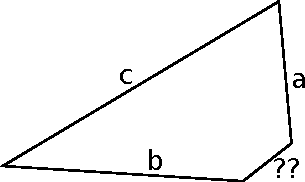
\includegraphics[width=.5\linewidth]{triangle2}
  \caption{Triangle drawn by my program. Note the 4th side.} \label{triangle2}
 \end{figure}
 
Unless there is a bug in my program, which is unlikely, this research indicates that the whole theory on triangles having 3 sides has been wrong for years, maybe decades.

 
 \chapter*{Conclusion}
 \addcontentsline{toc}{chapter}{Conclusion}
 
 
 
 
 
 % switch to A-B-C chaptering
 \appendix	
 
 \chapter{Proof of theorem \ref{theo}}
 \label{sec:prooftheorem}
 
 
 \begin{proof}
\eqref{theo} was already demonstrated in \cite{euclides300}.
\end{proof}
 
 \addcontentsline{toc}{chapter}{Bibliography}
 
 \bibliography{../biblio}
 
 
 
 
\end{document}
